\section{Background} \label{app:background}


We recall here the classical version of change of variable theorem for $\R^d$, see e.g. Thm. 40.7 of \citet{aliprantis1998principles}.
\begin{theorem}[Change of Variables]\label{thm:change-of-variable}
Let $V$ be an open set in $\R^d$ and $Q:\R^d \to \R^d$ be an injective continuosly differentiable map. Let $f \in L^1(V)$. Denote by $\nabla Q(x) \in \R^{d\times d}$ the gradient of $Q$ for any $x \in \R^d$. Then, we have
$$\int_{Q^{-1}(V)} f(Q(x)) |\nabla Q(x)| dx = \int_{V} f(y) dy. $$
\end{theorem}


\subsection{Sobolev spaces}

We recall some basic properties of Sobolev spaces. The Sobolev space $H^m(Z)$ for $m > 0$ and an open set $Z \subseteq \R^d$ is defined as follows \cite{adams2003sobolev}
$$H^m(Z) = \big\{f \in L^2(\R^d) ~\big|~ \|f\|_{H^m(Z)}\big\} < \infty\big\}, \quad \|f\|^2_{H^m(Z)} = \sum_{\alpha_1+\dots+\alpha_d \leq m} \int_{Z} \left|\frac{\partial^{\alpha_1 + \dots + \alpha_d} f(x)}{\partial x_1^{\alpha_1} \dots \partial x_d^{\alpha_d}}\right|^2 dx.$$
Analogously, we define the space $H^m(Z, \R^t)$ for functions with output in $\R^t$, $t \geq 1$, with norm $\|f\|_{H^m(Z,\R^t)}^2 = \sum_{j=1}^t \|f_j\|_{H^m(Z)}^2$.
In the following theorem we collect some important properties of $H^m(Z)$ that will be useful for the proof of \cref{theorem:main-theorem}.
\begin{theorem}\label{thm:good-rkhs}
Let $m > d/2$ and $Z$ be an open set with locally Lipschitz continuous boundary. The following properties hold
\begin{enumthm}
    \item \label{thm:sobolev-containCinfty} $H^m(Z)$ is a Reproducing Kernel Hilbert space. Moreover, $H^m(Z) \subset C(Z)$, and, when $Z$ is bounded we have $f|_Z \in H^m(Z)$, for any $f \in C^m(\R^d)$.
    \item \label{thm:sobolev-restriction-extension} {\em Restriction and extension.}
    For any $u \in H^m(\R^d)$, it holds that $u|_Z \in H^m(Z)$ and $\|u|_Z\|_{H^m(Z)} \leq c_1 \|u\|_{H^m(\R^d)}$. Moreover, for any $u \in H^m(Z)$ there exists a function $E_Z[u] \in \hh(\R^d)$ such that  $(E_Z[u])|_Z = u$ and $\|E_Z[u]\|_{H^m(\R^d)} \leq c_2\|u\|_{H^m(Z)}$. The constants $c_1,c_2$ depend only on $Z, m, d$.
    \item \label{thm:sobolev-pointwise-product} {\em Pointwise product.}
    For any $u, v \in H^m(Z)$ we have $u \cdot v \in H^m$. In particular, there exists $c_0 > 0$ depending only on $Z, m, d$ such that $\|u \cdot v\|_{H^m(Z)} \leq c_0 \|u\|_{H^m(Z)}\|v\|_{H^m(Z)}$.
\end{enumthm}
\end{theorem}
\begin{proof}
The space $H^m(\R^d)$ is a RKHS due to the characterization of the norm with respect to the Fourier transform \cite{wendland2004scattered}. The space $H^m(Z)$ is a RKHS since any restriction of a RKHS to a subset of the set of definition is still a RKHS \cite{aronszajn1950theory}. The inclusions derive directly by the definition of the $H^m$ norm \citep[see][for more embeddings of Sobolev spaces]{adams2003sobolev}.

The second point is a classical result on Sobolev space and is derived in \citet{adams2003sobolev}. The third point is equivalent to showing that the Sobolev spaces with $m > d/2$ are Banach algebras and it is derived in \citet{adams2003sobolev}. For the case $Z=\R^d$ an explicit derivation based on the Fourier transform is done in Lemma 10 of \citet{rudi2020finding}.
\end{proof}



\section{Proof of the more general version of Theorem~\ref{theorem:main-theorem}}


In the next subsection we introduce some preliminary results that will be necessary to prove the more general version of Theorem~\ref{theorem:main-theorem}, which is in the subsection \cref{sec:general-theorem}.

\subsection{Preliminary result on composition of Sobolev functions}\label{sec:functions}
The following theorem quantifies the fact that a Sobolev space with $m > d/2$ is closed with respect to composition with diffeomorphisms. There exists many abstract results about the closure of composition in Sobolev space in the literature  \citep[see \emph{e.g.}][]{bruveris2017regularity}. Here, however, we want a quantitative bound. We base our result on the explicit bound in \citet{bourdaud2011composition}. To obtain a final readable form we have to do a bit of slalom between restriction and extension between $Z$ and $\R^d$. Indeed, we need functions that are equivalent to the functions of interest on $Z$, but whose norm does not diverge when going to $\R^d$. For example, constant functions don't belong to $H^m(\R^d)$, but for us it is enough to have a function that is equal to a constant on $Z$ and that goes to zero at infinity fast enough to have finite $H^m(Z)$ norm.


\begin{theorem}[Smooth composition]\label{thm:sobolev-smooth-composition}
 Let $m > d/2$. Let $Q:\R^d \to \R^d$ be an invertible $m$-times differentiable map whose inverse has continuous Lipschitz derivative. Let $Z$ be open bounded set with Lipschitz boundary and a compact $\Omega$ such that $\Omega \subset Z$ and $Q^{-1}(\Omega)\subset Z$. Assume also, without loss of generality, that $0$ is in the interior of $\Omega$. For any $h \in H^m(\R^d)$ supported on $\Omega$ the following holds:
 \begin{enumerate}
     \item there exists $b \in H^m(\R^d)$ satisfying $b(x) = h(Q(x))$ for any $x \in Q^{-1}(\Omega)$.
     \item if $h(x) = 0$ for any $x \in \R^d\setminus \Omega$, then $b(x) = 0$ for any $x \in \R^d \setminus Q^{-1}(\Omega)$,
     \item the norm of $b$ is controlled by
\eqal{
\|b\|_{H^m(\R^d)} & ~\leq~ C\, \|h\|_{H^m(Z)}\, d_{\Omega, Q}^{-m-d/2} \, (1 + \|Q\|_{H^m(Z, \R^d)} + D^m + L^m),
}
\end{enumerate}
where $d_{\Omega,Q} := \min[1,~d_H(Q^{-1}(\Omega), Q^{-1}(Z) \cap Z)]$, $d_H(A,B)$ is the Haussdorff distance between two sets $A, B$ and $D := \textrm{diam}(Z)$, $L = \max_{x \in Z} \|\nabla Q (x)\|$, while $C$ depends only on $d, m, Z$.
\end{theorem}
\begin{proof}

To apply \citet{bourdaud2011composition} we need a function such that $h(0) = 0$. With this aim, we rewrite $h \circ Q$ as
$$h \circ Q = h(0) + ((h-h(0)) \circ Q).$$
\paragraph{Step 1. Construction of $b$.} Denote by $U$ the open set $U = Q^{-1}(Z) \cap Z$. Note that the set is not empty since, by construction, $Q^{-1}(\Omega) \subset U$.
Define $\tilde{Q} = E_{Z}[Q|_{Z}]$, i.e. the extension to the whole $\R^d$ of the restriction of $Q$ on the set $Z$ (restriction and extension done componentwise). By the first point we have that $Q|_{Z}$ belongs to $H^m(Z,\R^d)$ and, by the second point, that $\tilde{Q}$ belongs to $H^m(\R^d, \R^d)$ and moreover $\tilde{Q}(x) = Q(x)$ for any $x \in Z$.
Denote by $s = h(0) \in C^\infty(\R^d)$ the constant function equal to $h(0)$ everywhere on $\R^d$. In particular, note that $s|_Z \in H^m(Z)$ via \cref{thm:sobolev-restriction-extension}. Denote by $\tau$, the extension of $s|_Z$ to $\R^d$, i.e., $\tau = E_Z[s|_Z]$. Denote by $u$, the function $u = h|_Z - s|_Z$ and by $\tilde{u} \in H^m(\R^d)$ the function $\tilde{u} = E_{Z}[h|_Z - s|_Z]$. Note that $\tilde{u}(x) = h(x) - h(0)$ for any
$x \in Z$, and, in particular for any $x \in \Omega$. Define by $\rho$ the $C^\infty(\R^d)$ function that is $1$ on $Q^{-1}(\Omega)$ and $0$ on $\R^d \subseteq U$.

Now define,
$$b ~~=~~ \rho ~\cdot~ (\tau ~+~ \tilde{u} \circ \tilde{Q}).$$
Denote by $\tilde{b}$ the function $\tilde{b} = \tau + \tilde{u} \circ \tilde{Q}$. We have that $\tilde{b}(x) = h(Q(x))$ for any $x \in U$. Since $Q(U) \subseteq Z$ and that $\tilde{h}(x) = h(x), \tilde{Q}(x) = Q(x)$ for any $x \in Z$. In particular, since $\tilde{b}(x) = 0$ for all $x \in U \setminus Q^{-1}(\Omega)$ and by definition of $\rho$, we have: (a)  $\rho \cdot \tilde{b} = \tilde{b} = h(Q(x))$ on $Q^{-1}(\Omega)$, (b) $\rho \cdot \tilde{b} = 0$ on $U Q^{-1}(\Omega)$; (c) $\rho \cdot \tilde{b} = 0$ and $0$ on $\R^d \setminus U$. Then $b = \rho \cdot \tilde{b} = h(Q(x))$ for any $x \in \R^d$.



\paragraph{Step 2. Bound of $b$.}
Now, let us bound the norm of $b$. By applying \cref{thm:sobolev-pointwise-product} we have
\eqal{\label{eq:bound-composition}
\|b\|_{H^m(\R^d)} & \leq c \|\rho\|_{H^m(\R^d)}(\|\tau\|_{H^m(\R^d)} ~+~ \|\tilde{u} \circ \tilde{Q}\|_{H^m(\R^d)}).
}
The bound for $\tau$ is obtained applying \cref{thm:sobolev-restriction-extension} and the definition of $H^m(Z)$ norm, as follows,
$$\|\tau\|_{H^m(\R^d)} \leq c_2(Z) \|s|_Z\|_{H^m(Z)} = c_2 h(0) \textrm{vol}(Z)^{1/2}.$$
Now we bound the norm $\|\tilde{u} \circ \tilde{Q}\|_{H^m(\R^d)}$ with respect to the norms of $\tilde{u}$ and $\tilde{Q}$. We use a result on the composition of Sobolev functions \citep[][Theorem 27]{bourdaud2011composition} that is highly technical, but allows to highlight the quantities of interests for us. For a more extensive treatment of the topic see for example \citet{runst2011sobolev}. Since $\tilde{u}(0) = 0$ by construction, by applying Theorem 27 of \citet{bourdaud2011composition} with $p=2$ and considering that their norm $\|\cdot\|_{\dot{W}_{E^p}^m}$ is bounded by $\|\cdot\|_{H^m(\R^d)}$ and analogously $\|\cdot\|_{\dot{W}^1_{mp}} \leq \|\cdot\|_{\dot{W}^1_{\infty}} \leq \|\cdot\|_{W^1_\infty(\R^d)}$,
\eqal{
\|\tilde{u} \circ \tilde{Q}\|_{H^m(\R^d)} \leq c (\|\tilde{u}\|_{H^m(\R^d)} + \|\tilde{u}\|_{\dot{W}^1_\infty(\R^d)})(\|\tilde{Q}\|_{H^m(\R^d, \R^d)} + \|\tilde{Q}\|^m_{\dot{W}^1_\infty(\R^d, \R^d)})
}
Here $\|z\|_{\dot{W}^1_\infty(A, \R^d)} = \sup_{x \in A, j \in \{1,\dots,t\}} \|\nabla z_j\|$ for any differentiable $z:A \to \R$ and open set $A$.
Now to conclude, note that
$$\|\tilde{u}\|_{H^m(\R^d)} = \|E_{Z}[h|_Z - s|_Z]\|_{H^m(\R^d)} \leq c_2 \|h|_Z - s|_Z\|_{H^m(Z)} \leq c_2 \|h\|_{H^m(Z)} + c_2 h(0) \textrm{vol}(Z)^{1/2},$$
moreover
$$\|\tilde{Q}\|_{H^m(\R^d,\R^d)} = \|E_Z(Q|_Z)\|_{H^m(\R^d, \R^d)} \leq c_2 \|Q|_Z\|_{H^m(Z, \R^d)}.$$
Note also that for the Sobolev space $W^1_\infty$ there exists the same type of result as \cref{thm:sobolev-restriction-extension} and for the same extension operator defined in \cref{thm:sobolev-restriction-extension} (which is a {\em total extension operator}, see e.g. the Stein extension theorem, Thm 5.4 page 154 of \citealp{adams2003sobolev}), so, as above, we have
$$\|\tilde{u}\|_{W^1_\infty(\R^d)} \leq c_2 \|h\|_{W^1_\infty(Z)} + c_2 h(0),$$
and also
\eqals{
\|\tilde{Q}\|_{W^1_\infty(\R^d,\R^d)}  &\leq c_2 \|Q|_Z\|_{W^1_\infty(Z, \R^d)} \\&= c_2\sup_{x \in Z} \max(\|Q(x)\|, \|\nabla Q(x)\|) \\&\leq  c_2\textrm{diam}(Z) + c_2 \sup_{x \in Z} \|\nabla Q (x)\|.
}
Substituting the six bounds above in \cref{eq:bound-composition}, we obtain
\begin{align*}
\|b\|_{H^m(\R^d)} \leq &c \|\rho\|_{H^m(\R^d)}(c_2 h(0) \textrm{vol}(Z)^{1/2}\\
& ~+~ c^\prime ( \|h\|_{H^m(W)} + \|h\|_{W^1_\infty(Z)} + h(0) c^{\prime\prime})(\|Q|_Z\|_{H^m(Z, \R^d)} + D^m + L^m)),
\end{align*}
where $D =\textrm{diam}(Z)^m $, $L = \sup_{x \in Z} \|\nabla Q (x)\|$ and $c^\prime = c c_2^2 (1 + 2^m c_2^{m-1})$, $c^{\prime\prime}=1+\textrm{vol}(Z)^{1/2}$, with $c, c_2$ depending only on $d, m, Z$.
The final result is obtained considering that $x A + d (B + y A) R \leq (1+ d + d y)(B+A)(1+R)$ for any $x,y,d,A,B, R \geq 0$, and applying this result with $x=c_2(Z)\textrm{vol}(Z)^{1/2}$, $A = h(0)$, $d = c^\prime$, $B = \|h\|_{H^m(Z)} + \|h\|_{W^1_\infty(Z)}$, $y= c^{\prime \prime}$, $R = \|Q|_Z\|_{H^m(Z, \R^d)} + D^m + L^m$. In particular, in the final result, the constant $C$ corresponds to $C = 3(1+ d + d y)$ and we used the fact that $h(0) \leq \|h\|_{W^1_\infty(Z)} \leq \|h\|_{H^m(Z)}$, then $\|h\|_{H^m(Z)} + \|h\|_{W^1_\infty(Z)} + h(0) \leq 3 \|h\|_{H^m(Z)}$.


\paragraph{Step 3. The norm of $\rho$}.  Let $A_{t}$ be the set $A_{t} = \{x ~|~ \min_{y \in Q^{-1}(\Omega)} \|x-y\| \leq t\}$. Let $\eta = d_H(Q^{-1}(\Omega), \overline{U})$, i.e., the Haussdorff distance between the sets $Q^{-1}(\Omega)$ and $\overline{U}$, corresponding to the largest $\eta$ for which $A_\eta \subseteq U$. Note that $\eta > 0$ since $Q^{-1}(\Omega)$ is compact, while $U$ is open and $Q^{-1}(\Omega) \subset U$. The fact that $\eta > 0$ implies that for any $\eta^\prime < \eta$ it holds that $A_{\eta^\prime} \subset U$.

The function $\rho$ is obtained by the convolution of the indicator function $1_{A_{\eta/2}}$ with the bump function $\psi_{\eta/2}(x) =  (\eta/2)^{-d} \psi(x/(\eta/2))/S$ where $S = \int_{\R^d} \psi(x) dx$ and $\psi$ is an infinitely smooth non-zero non-negative function that is $0$ on $\|x\| \geq 1$ as for example $\psi(x) = \exp(-1/(1-\|x\|^2)_+)$ for any $x \in \R^d$, where $(z)_+ = \max(0,z)$. In particular, since (a) $\|f(y-\cdot)\|_{H^m(\R^d)} = \|f\|_{H^m(\R^d)}$ for any $y \in \R^d$, by construction of the norm $H^m(\R^d)$, and (b) $\|t^{-d} f(\cdot/t)\|_{H^m(\R^d)} \leq c_6 t^{-d/2} \max(1,t^{-m}) \|f\|_{H^m(\R^d)}$ (see, e.g., Proposition 3 of \citealp{runst2011sobolev}) we have
\eqals{
\|\rho\|_{H^m(\R^d)} &\leq \int_{A_{\eta/2}} \|\psi_\eta(y-\cdot)\|_{H^m(\R^d)} dy  \leq \textrm{vol}(A_{\eta/2}) \|\psi_\eta\|_{H^m(\R^d)} \\
& \leq c_6 \|\psi\|_{H^m(\R^d)} ~ \textrm{vol}(A_{\eta/2}) ~ (\eta/2)^{-d/2} \max(1,(\eta/2)^{-m}).
}
To conclude note that $\textrm{vol}(A_\eta) \leq \textrm{vol}(Z)$, since $A_{\eta/2} \subset U \subseteq Z$.
\end{proof}


\begin{lemma}[Existence and norm of $\tilde{q} \in H^m(\R^d)$]\label{lm:existence-q}
Let $\mu$ be an infinitely differentiable function, with compact support $\Omega \subset \R^d$. Let $Q:\R^d \to \R^d$ be a $C^{m+1}$ diffeomorphism. Let $Z$ be an open bounded set with Lipschitz boundary and such that $\Omega \subset Z$ and $Q^{-1}(\Omega) \subset Z$. Moreover, assume without loss of generality that $0$ is in the interior of $\Omega$.
For any $h \in H^m(\R^d)$, there exists a function $\tilde{q} \in H^m(\R^d)$ satisfying
\eqal{\label{eq:q-equivalence}
 \tilde{q}(y) = \begin{cases} h(Q(y)) \mu(Q(y)) |\nabla Q(y)| &  y \in Q^{-1}(\Omega) \\
 0 & y \in \R^d \setminus Q^{-1}(\Omega)
 \end{cases}.
}
In particular, let $b \in H^m(\R^d)$ be defined according to \cref{thm:sobolev-smooth-composition}, then
$$ \|q\|_{H^m(\R^d)} \leq C^\prime \|h\|_{H^m(\R^d)}\|\mu\|_{H^m(\R^d)} d_{\Omega,Q}^{-m-d/2} \|\nabla Q\|_{H^m(Z, \R^d)}^d (1 + \|Q\|_{H^m(Z, \R^d)} + D^m + L^m),
$$
the constant $C$ depends only on $d, m, Z$, while $d_{\Omega, Q} := \min[1, d_H(Q^{-1}(\Omega), Q^{-1}(Z) \cap Z)$ and $d_H(A, B)$ is the Haussdorff distance between two sets $A, B$.
\end{lemma}
\begin{proof}
Let $h \in H^m(\R^d)$ and $\tilde{\mu}$ to be the extension of $\mu$ on $\R^d$ (which corresponds to $\tilde{\mu}(x) = \mu(x)$ for any $x \in \Omega$ and $\tilde{\mu}(x) = 0$ for $x \in \R^d \setminus \Omega$). Define the function $s(x) = h \cdot \tilde{\mu}$ and note that $s \in H^m(\R^d)$ since it is the product of two functions in $H^m(\R^d)$ (see \cref{thm:sobolev-pointwise-product}).

Second, note that the function $r = (|\nabla Q|)|_Z \in H^m(Z)$ since (a) the map $\nabla Q$ belongs to $C^{m+1}(\R^d, \R^d)$ so its entries $(\nabla Q)_{i,j}|_Z$ belong to $H^m(Z)$ (see \cref{thm:sobolev-containCinfty}); and (b) the determinant of a matrix, by the Leibniz formula, is defined in terms of sums and products of its entries and $H^m(Z)$ is closed with respect to multiplication, by \cref{thm:change-of-variable}. To quantify its norm let's write explicitly the Leibniz formula \cite{trefethen1997numerical},
$$ |\nabla Q| = \sum_{\sigma \in S_d} \mathrm{sgn}(\sigma) \prod_{i=1}^d e_{\sigma_i}^\top\frac{\partial Q(x)}{\partial x_i},$$
where $\mathrm{sgn}(\sigma) \in \{-1,1\}$, $S_n$ is the set of permutations of of $d$ elements and $e_1,\dots,e_d$ is the canonical basis of $\R^d$. Note, in particular, that, by the equation above, since $|S_d| = d!$ and that $\|e_{\sigma_i}^\top\frac{\partial Q(x)}{\partial x_i}\|_{H^m(Z)} \leq \|\nabla Q\|_{H^m(Z,\R^d)}$, we have that
$$\|r\|_{H^m(Z)} \leq d! \|\nabla Q\|_{H^m(Z, \R^d)}^d.$$

Now consider the function $b \in H^m(\R^d)$ defined according to \cref{thm:sobolev-smooth-composition} we have that $b(x) = s(Q(x))$ for any $x \in \R^d$. Now, define $\tilde{q}$ as follows
$$ \tilde{q} = b  \cdot  E_Z[r].$$
The function $\tilde{q}$ is in $H^m(Z)$, since it is the product of two functions in $H^m(Z)$ (see \cref{thm:sobolev-pointwise-product} and $r \in H^m(Z)$ (see \cref{thm:sobolev-restriction-extension}). Note, in particular, that \cref{eq:q-equivalence} holds, by construction. To conclude, note that, by applying \cref{thm:sobolev-pointwise-product} and \cref{thm:sobolev-restriction-extension}, we have
\begin{align*}
\|q\|_{H^m(\R^d)} &\leq c_0 \|E_Z[r]\|_{H^m(\R^d)} \|b\|_{H^m(\R^d)} \\&\leq c_0 c_2 \|r\|_{H^m(Z)} \|b\|_{H^m(\R^d)} \\&\leq d! c_0 c_2 \|\nabla Q\|_{H^m(Z,\R^d)}^d \|b\|_{H^m(\R^d)}.
\end{align*}
To conclude, we bound $b$ according with \cref{thm:sobolev-smooth-composition}, obtaining
$$\|b\|_{H^m(\R^d)} \leq C\, \|s\|_{H^m(W)}\, d_{\Omega, Q}^{-m-d/2}(1 + \|Q\|_{H^m(Z, \R^d)} + D^m + L^m), $$
and $\|s\|_{H^m(W)} \leq \|s\|_{H^m(\R^d)} \leq c_0 \|h\|_{H^m(\R^d)}\|\mu\|_{H^m(\R^d)}$, by \cref{thm:sobolev-pointwise-product}.
\end{proof}

\subsection{Proof of the general version of Theorem~\ref{theorem:main-theorem}}\label{sec:general-theorem}

\cref{theorem:main-theorem} is a particular case of the following theorem

\begin{theorem}\label{thm:general-theorem}
Let $X \subset \R^d$ be an open bounded set with Lipschitz boundary. Let $\mu \in C^\infty(\R^d)$ with compact support $\Omega \subset X$. Let the RKHS $\hh$ be $\hh = H^m(\R^d)$, i.e. the Sobolev space of smoothness $m$, with $m > d/2$. Denote by ${\cal F}$ the RKHS induced by the kernel $k_Y$ on $Y$, that we assume uniformly bounded. Then for any $C^{m+1}$ diffeomorphism $Q$ on $\R^d$ satisfying $Q^{-1}(\Omega) \subset X$, we have that for all $f, g$ measurable functions,
\eqals{
 g(x) = (f \circ Q)(x), ~~ \forall x \in Q^{-1}(\Omega) \qquad \textrm{implies} \qquad D(f, g) ~~\leq~~ \lambda ~ C_{\mu} C_{Q},
}
where $C_\mu = \|\mu\|_{H^m(\R^d)}$, and $C_Q$ is defined in \cref{eq:def-CQ} below and depends only on $\Omega, X, Q, d, m$.
\end{theorem}
\begin{proof}
Now we have all the elements to prove the main theorem of the paper. Let $\tilde{q}$ as defined in \cref{lm:existence-q}, with $Z = X$. Moreover, let
$v \in {\cal F}$, where ${\cal F}$ is the reproducing kernel Hilbert space associated to the kernel $k_Y$ which is bounded by assumption. Then for any continuous $f$, we have that $v \circ f$ is continuous and bounded.
Denote by $\Theta_{f,g}(h,v,q)$ the quantity
$$\Theta_{f,g}(h,v,q) := \int_X v(f(x)) h(x) \mu(x) dx - \int_X v(g(y)) q(y) dy.$$
%
\paragraph{Step 1. Simplifying $\Theta_{f,g}(h,v,\tilde{q})$.}
Since $\mu$ is supported on $\Omega \subseteq X$, by assumptions, we have
$$\int_X v(f(x)) h(x) \mu(x) dx = \int_\Omega v(f(x)) h(x) \mu(x) dx.$$
Moreover, by expanding the characterization of $\tilde{q}$ in \cref{eq:q-equivalence}, we have that $\tilde{q}(x) = 0$ for any $x \in \R^d \setminus Q^{-1}(\Omega)$, since $Q^{-1}(\Omega) \subseteq X$, we have
\eqals{
\int_X v(g(y)) \tilde{q}(y) dy &= \int_{Q^{-1}(\Omega)} v(g(y)) h(Q(y)) \mu(Q(y)) |\nabla Q(y)| dy,\\
& = \int_{Q^{-1}(\Omega)} v(f(Q(y))) h(Q(y)) \mu(Q(y)) |\nabla Q(y)| dy,
}
where we used in the last step that $g(y) = f(Q(y))$ for any $y \in Q^{-1}(\Omega)$, which is now the domain of integration.
%
\paragraph{Step 2. Applying the Change of Variable theorem.}
Note that the function $\tilde{q}$ is continuous since $H^m(\R^d)$ is subset of continuous functions. By applying the change of variable theorem we have
$$\int_{Q^{-1}(\Omega)} v(f(Q(x))) h(Q(x)) \mu(Q(x)) |\nabla Q(x)| dx = \int_{\Omega} v(f(y)) h(y) \mu(y) dy.$$
Then, by using the characterizations in Step 1, we have
\eqals{
\Theta_{f, g}(h,v,\tilde{q}) & = \int_X v(f(x)) h(x) \mu(x) dx - \int_X v(g(y)) \tilde{q}(y) dy \\
& = \int_\Omega v(f(x)) h(x) \mu(x) dx - \int_{Q^{-1}(\Omega)} v(f(Q(y))) h(Q(y)) \mu(Q(y)) |\nabla Q(y)| dy\\
& = 0.
}

\paragraph{Step 3. Bound on $D_\la(f, g)$.}
Now, denote by $\hh$ the set $H^m(\R^d)$. Since $\tilde{q} \in \hh$, and $\Delta_{f, g}(h,v,\tilde{q}) = 0$, we have that
\eqal{
D_\la(f, g) = \max_{\|h\|_{\hh} \leq 1} \min_{q \in \hh} \max_{\|v\|_{\cal F} \leq 1} |\Theta_{f, g}(h,v,q)|^2 + \la \|q\|^2_{\hh} & \leq \max_{\|h\|_{\hh} \leq 1} \max_{\|v\|_{\cal F} \leq 1} |\Theta_{f, g}(h,v,\tilde{q})|^2 + \la \|\tilde{q}\|^2_{\hh} \\
& = \max_{\|h\|_{\hh} \leq 1} \la \|\tilde{q}\|^2_{\hh}.
}

\paragraph{Step 4. Simplifying $\|\tilde{q}\|_{H^m(\R^d)}$.}
We bound $\|\tilde{q}\|_{H^m(\R^d)}$ as in \cref{lm:existence-q}, where $b$ is bounded according to \cref{thm:sobolev-smooth-composition},
$$\|\tilde{q}\|_{H^m(\R^d)} \leq C^\prime\|h\|_{H^m(\R^d)} C_\mu C_Q,$$
where $C_\mu := \|\mu\|_{H^m(\R^d)}$ and
\eqal{\label{eq:def-CQ}
C_Q  ~~:= ~~ d_{\Omega, Q}^{-m - d/2} ~ \|\nabla Q\|_{H^m(X, \R^d)}^d (1 + \|Q\|_{H^m(X, \R^d)} + D^m + L^m),
}
where $D := \textrm{diam}(X)$,  $L = \max_{x \in X} \|\nabla Q (x)\|$ and $d_{\Omega, Q} := \min[1, d_H(Q^{-1}(\Omega), Q^{-1}(X) \cap X)]$ and $d_H(A, B)$ is the Haussdorff distance between two sets $A, B$.

The final result is obtained by considering that we are optimizing with the constraint $\|h\|_{H^m(\R^d)} \leq 1$.
\end{proof}


\section{Proof of closed form of $D_\la$ and computational results}\label{sec:additional-proofs}

In the next lemma, we prove some important properties useful for the characterization of $D_\la$ in terms of $F_\mu, G$.


\begin{lemma}\label{lm:explicit-Fmu-G}
Let $X \subset \R^d$ be an open bounded set. The linear operators $F_\mu, G$ defined above are compact and trace class.
Moreover, for any $h, q \in \hh$ and $v \in {\cal F}$, we have
\eqals{
\scal{v}{F_\mu h}_{\cal F} &= \int_X v(f(x)) h(x) \mu(x) dx, \\
\scal{v}{G q}_{\cal F} &= \int_X v(f(x)) q(x) dx.
}
\end{lemma}
\begin{proof}
Since $k_Y$ is bounded, and $f, g$ are measurable, then $\Phi(f(\cdot)):X \to {\cal F}$ is bounded and measurable. Since $\mu \in C^\infty(\R^d)$ by assumption $X$ is bounded and $h$ is bounded and continuous since it belongs to $\hh$ and $k_X$ is bounded and continuous, so $$J := \int_X \|\Phi(f(x))\|_{\cal F} \|\psi(x)\|_{\hh}|\mu(x)| \dd x < \infty$$. This guarantees the existence of the following Bochner integral
$$F_\mu:=\int_X \Phi(f(x)) \otimes \psi(x) \mu(x)\dd x ~~ \in {\cal F} \otimes {\hh}.$$
In particular, denoting by $\|\cdot\|_*$ the trace norm, i.e. $\|A\|_* = \tr(\sqrt{A^*A})$, and recalling that
$\|u \otimes v\|_* = \tr(\sqrt{(u \otimes v)^*(u \otimes v)}) = \|u\|_{F}\|v\|_{\hh}$ for any $u \in {\cal U}, v \in {\cal V}$ and any two separable Hilbert spaces ${\cal U}, {\cal V}$, we have
$$\|F_\mu\|_* \leq \int_X \|\Phi(f(x)) \otimes \psi(x)\|_* |\mu(x)| dx = \int_X \|\Phi(f(x))\|_{\cal F} \|\psi(x)\|_\hh |\mu(x)| dx =: J < \infty.$$
Then $F_\mu$ is trace class.
The same reasoning hold for $G$, considering that $$\int_X \|\Phi(f(x))\|_{\cal F} \|\psi(x)\|_{H} \dd x < \infty$$ since $X$ is compact.
\end{proof}

\subsection{Proof of \cref{theorem:closed-form}}\label{sec:proof-closed-form}
\begin{proof}
We have seen in \cref{lm:explicit-Fmu-G}, that since $X$ is a bounded set, then $F_\mu$ and $G$ are trace class and, by the representer property
\eqals{
\scal{v}{F_\mu h}_{\cal F} &= \int_X v(f(x)) h(x) \mu(x) dx,\\
\scal{v}{G q}_{\cal F} &= \int_X v(f(x)) q(x) dx
}
Using this result and considering the linearity of the inner product and the variational characterization of the Hilbert norm (i.e. $\|u\|_{\cal F} = \max_{\|v\|_{\cal F} \leq 1} |\scal{v}{u}|_{\cal F}$  for any $u \in {\cal F}$), we have
\eqals{
\Delta_{f,g}(h,q) &= \max_{\|v\|_{\cal F} \leq 1} |\scal{v}{F_\mu h}_{\cal F}  - \scal{v}{G q}_{\cal F}|^2 \\
& = \max_{\|v\|_{\cal F} \leq 1} |\scal{v}{F_\mu h - G q}_{\cal F}|^2 \\
& = \|F_\mu h - G q\|_{\cal F}^2,
}
for any $h, q \in \hh$. From which we characterize $D_\lambda$ as
\eqal{
D_\lambda(f, g) = \max_{\norh{h}\leq 1} \min_{q\in\hh} \norf{F_\mu h - G q}^2 + \lambda \norh{q}^2.
}
Now, we prove that the problem above has a characterization in terms of the operatorial norm of a given operator.
First, notice that $q\mapsto \norf{Fh - Gq}^2 + \lambda \norh{q}^2$ is $2\lambda$-strongly convex. It has a unique global minimizer $q^*(h)$ which is also a critical point. This leads to $q^*(h) = ZFh$ where $Z = (GG^* + \lambda I)^{-1}G^*$. Here $GG^* + \lambda I$ is a positive linear operator. Thus, it is invertible.

So far, we have shown that: \eqal{D(f, g) = \max_{\norh{h}\leq 1}\norf{Fh - GZFh}^2 + \lambda \norh{ZFh}^2.}

Rewriting both squared norms as scalar products in $\mathcal F$ and $\hh$ and using the adjoint operators, we have that:
$\norf{Fh - GZFh}^2 + \lambda \norh{ZFh}^2 = \langle h, Th\rangle_\hh$ with $T = F^*(I - Z^*G^*)(I-GZ)F + \lambda F^* Z^*ZF$. Thus, we have rewritten $D$ as the operator norm of $T$: \eqal{D(f, g) = \max_{\norh{h}\leq 1}\langle h, Th\rangle_\hh = \norop{T}.}

We can now simplify $T$. Recall that for any bounded operator $A$, $A(A^*A + \lambda I)^{-1} = (AA^* + \lambda I)^{-1}A$ and $(A + \lambda I)^{-1}A = I - \lambda(A + \lambda I)^{-1}.$

Thus, $GZ = Z^*G^*= G(G^*G + \la I) ^{-1} G^*= (GG^* + \la I)^{-1}GG^* = I - \la (GG^* + \la I)^{-1}.$ Similarly,
\eqal{Z^*Z &= G(G^*G + \la I) ^{-1}(G^*G + \la I) ^{-1} G^* = (GG^* + \la I) ^{-1}GG^*(GG^* + \la I) ^{-1}\\
&= (I - \la (GG^* + \la I)^{-1}(GG^* + \la I) ^{-1}= (GG^* + \la I) ^{-1} -\la (GG^* + \la I) ^{-2}.
}

Replacing these expression in $T$, we obtain:
\eqal{
T &= \la^2F^*(GG^* + \la I)^{-1})(GG^* + \la I)^{-1})F + \lambda F^* \left[(GG^* + \la I) ^{-1} -\la (GG^* + \la I) ^{-2}\right]F\\
  &= \la F^*(GG^* + \la I)^{-1}F.
}
Finally,
\eqal{D_\lambda(f, g) = \norop{T} = \la \norop{F^*(G^* + \la I)^{-1} F}= \la\norop{(GG^* + \la I)^{-1/2}F}^2.}
\end{proof}



\subsection{Proof of \cref{lm:widehatD}}


Before proceeding with the proof of \cref{lm:widehatD}, we introduce some operators, that will be useful also in the rest of the paper. We recall that for this set of results we are assuming that the kernel $k_X$ is universal. This implies that the kernel matrix $K_{\tilde{X},\tilde{X}}$ is invertible and so $R_{\tilde{X}}$ exists and is invertible. The same holds for $R_{\tilde Y}$.

\begin{definition}[The operators $S, V:\hh\to\R^{M_X}$ and $Z, U: {\cal F} \to \R^{M_Y}$]\label{def:operators}
First define $S:\hh \to \R^{M_X}$ as
\eqals{
Su & = (\scal{\psi(\tilde{x}_1)}{u}_\hh, \dots, \scal{\psi(\tilde{x}_{M_X})}{u}_\hh) \in \R^{M_X}, \quad S^* \alpha = \sum_{i=1}^{M_X} \alpha_i \psi(\tilde{x}_i),
}
for all $u \in \hh$ and $\alpha \in \R^{M_X}$.
Analogously define $Z:{\cal F} \to \R^{M_Y}$ as
\eqals{
Zv & = (\scal{\Phi(\tilde{y}_1)}{v}_{\cal F}, \dots, \scal{\Phi(\tilde{y}_{M_Y})}{v}_{\cal F}) \in \R^{M_Y}, \quad Z^* \beta = \sum_{i=1}^{M_Y} \beta_i \Phi(\tilde{y}_i),
}
for all $v \in {\cal F}$ and $\beta \in \R^{M_Y}$.
Moreover, define $V, U$ as
$$V = R^{-\top}_{\tilde X} S, \qquad V = R^{-\top}_{\tilde Y} Z.$$
\end{definition}

\begin{remark}\label{rem:operators}
We recall the following basic facts about the operator above, together with a short proof, when needed.
\begin{enumerate}
    \item The range of $S^*$ is $\textrm{span}(\psi(x_1),\dots,\psi(x_{M_X})$,
    \item $S$ is full rank and  $SS^* = K_{\tilde{X} \tilde{X}}$,
    \item $R_{\tilde{X}}^\top R_{\tilde{X}} = K_{\tilde{X} \tilde{X}}$, since $R_{\tilde{X}}$ is the upper-triangular Cholesky of $K_{\tilde{X} \tilde{X}}$.
    \item  $VV^* = I$, indeed, $VV^*  = R^{-\top}_{\tilde X} S S^* R^{-1}_{\tilde X}  = R^{-\top}_{\tilde X} K_{\tilde{X} \tilde{X}} R^{-1}_{\tilde X}  = R^{-\top}_{\tilde X} R_{\tilde{X}}^\top R_{\tilde{X}} R^{-1}_{\tilde X} = I.$
    \item $V$ is a partial isometry, since $VV^* = I$ and it is full rank, since it is the product of two full rank operators.
    \item $P_{\tilde{X}} = V^*V$, indeed, $V^*V$ is a projector and the range of $V^*$ is the range of $S^*$ that is $\textrm{span}(\psi(x_1),\dots,\psi(x_{M_X})$.
\end{enumerate}
For the same reasons, we have that: (a) The range of $Z^*$ is $\textrm{span}(\Phi(\tilde{y}_1),\dots,\Phi(\tilde{y}_{M_Y})$ (b) $Z$ is full rank and $ZZ^* = K_{\tilde{Y} \tilde{Y}}$ (c) $R_{\tilde{Y}}^\top R_{\tilde{Y}} = K_{\tilde{Y} \tilde{Y}}$ (d) $UU^* = I$ (e) $U$ is a partial isometry (f) $P_{\tilde{Y}} = U^*U$.
\end{remark}

Now we are ready to state the proof of \cref{lm:widehatD}.

\begin{proof}
First, note that since $\|A\|_{\mathrm{op}}^2 = \|A^*A\|_{\mathrm{op}}$ for any bounded linear operator $A$, we have
$$
\widehat{D}_\la = \la \|P_{\tilde{X}} F_{\mu, N}^* P_{\tilde{Y}} (P_{\tilde{Y}} G_N P_{\tilde{X}} G_N^*P_{\tilde{Y}} + \la)^{-1} P_{\tilde{Y}} F_{\mu, N} P_{\tilde{X}} \|_{\mathrm{op}}.
$$
From \cref{rem:operators} we recall that $P_{\tilde X} = V^*V$ where $V$ is a partial isometry defined in \cref{def:operators}. Analogously $P_{\tilde Y} = U^*U$ where $V$ is a partial isometry defined in \cref{def:operators}.
Now, we have $U(U^*BU + \la I)^{-1}U^* = (B + \la I)^{-1}$ for any positive semidefinite operator $B \in \R^{M_Y \times M_Y}$, since since $UU^*=I$ and so $U^*UU^* = U^*$, indeed
\eqals{
U(U^*BU + \la I)^{-1}U^*(B + \la I) &= U(U^*BU + \la I)^{-1}U^*(B + \la I)UU^* \\
& = U(U^*BU + \la I)^{-1}(U^*BU + \la U^*U)U^* \\
& = U(U^*BU + \la I)^{-1}(U^*BU + \la I)U^* -  \la U(U^*BU + \la I)^{-1}(I - U^*U)U^* \\
& = UU^* -  \la U(U^*BU + \la I)^{-1}(U^* - U^*UU^*) = I.
}
In particular, we will use now the result above. Let $C = U G_N P_{\tilde{X}} G_N^* U^*$. So,
\eqals{
\widehat{D}_\la & = \la \|V^* VF_{\mu, N}^* U^*U(U^*CU + \la I)^{-1} U^*U F_{\mu, N} V^* V \|_{\mathrm{op}}\\
& = \la \|V^* A^* (C + \la I)^{-1} A V \|_{\mathrm{op}}\\
& = \la \|A^* (C + \la I)^{-1} A \|_{\mathrm{op}}
}
where $A = U F_{\mu, N} V^*$ and we used the fact that $\|V^* T U\|_{\mathrm{op}} = \|T\|_{\mathrm{op}}$ for any couple of partial isometries such that $VV^* = I$ and $UU^* = I$.
By applying the definition of $U, V$ and $F_{\mu, N}$, we see that $A = \widehat{A}$ as in \cref{eq:widehatA}.
Indeed, by expanding the definitions of $U, V$ from \cref{def:operators} and denoting by $c_i \in \R^{M_Y}$ and $d_i \in \R^{M_X}$ respectively the vectors
$c_i = Z\,\Phi(f(x_i)) = \left(k_Y(\tilde{y}_1,f(x_i)), \dots,  k_Y(\tilde{y}_{M_Y},f(x_i)) \right)$ and
$d_i = S\psi(x_i) = \left(k_X(\tilde{x}_1,x_i), \dots,  k_X(\tilde{x}_{M_X},x_i) \right)$, we have
\eqals{
U F_{\mu, N} V^* &= \frac{v_X}{N}\sum_{i=1}^N (U\Phi(f(x_i))) \otimes (V\psi(x_i)) \mu(x_i)\\
& = \frac{v_X}{N}\sum_{i=1}^N R^{-\top}_{\tilde Y} \left((Z\Phi(f(x_i))) \otimes (S\psi(x_i))\right)R^{-1}_{\tilde X} \mu(x_i)\\
& = \frac{v_X}{N}\sum_{i=1}^N R^{-\top}_{\tilde Y} \left(c_i d_i^\top\right)R^{-1}_{\tilde X} \mu(x_i).
}
Note now, that by construction $c_i$ is the $i$-th column of $K_{\tilde{Y},f}$ while $d_i$ is the $i$-th row of the matrix $K_{X,\tilde{X}}$ for $i=1,\dots,N$. Denoting by $\diag{\hat{\mu}}$ the diagonal matrix whose $i$-th element of diagonal is $\mu(x_i)$, we have
$$ \sum_{i=1}^N \mu(x_i) \, c_i d_i^\top   = K_{\tilde{Y},f}\diag{\hat{\mu}}K_{X,\tilde{X}}.$$
From which have
$$
U F_{\mu, N} V^* = \frac{1}{N}R^{-\top}_{\tilde Y} K_{\tilde{Y},f}\diag{\hat{\mu}}K_{X,\tilde{X}} R^{-1}_{\tilde X} = \widehat{A}.
$$
To conclude, note that
$$C = U G_N P_{\tilde{X}} G_N^* U^* = (U G_N V^*) (V G_N^* U^*) = (U G_N V^*)\,(U G_N V^*)^*  ,$$
Analogously as we proved that $A = \widehat{A}$, we have that $U G_N V^* = \widehat{B}$, where $\widehat{B}$ is defined in \cref{eq:widehatB}. Then
$$\widehat{D}_\la = \la \|A^* (C + \la I)^{-1} A \|_{\mathrm{op}} = \la \|\widehat{A}^* (\widehat{B}\widehat{B}^* + \la I)^{-1} \widehat{A} \|_{\mathrm{op}}.$$
\end{proof}


\section{Proof of \cref{thm:appr-error-widehatD}}

Before proving the theorem, we need some preliminary lemmas

\begin{lemma}\label{lm:nystrom}
Let $\delta \in (0,1)$. Let $X \subseteq \R^d$ be an open bounded set with locally Lipschitz boundary. Let $k$ be a Sobolev kernel of smoothness $m$, with $m > d/2$ on $X$ and denote by $\hh$ and $\psi:X\to\hh$ the associated RKHS and canonical feature map. Let $\tilde{X} = \{\tilde{x}_1,\dots,\tilde{x}_M\} \subset X$ be $M$ points sampled independently and uniformly at random in $X$.
Denote by $P_{\tilde{X}}$ the projection operator whose range corresponds to $\textrm{span}\{\psi(\tilde{x}_1),\dots,\psi(\tilde{x}_M)\}$.
There exists $M_0$ such that for all $M \geq M_0$, the following holds with probability at least $1-\delta$:
\eqals{
\sup_{x \in X}\|(I-P_{\tilde{X}})\psi(x)\|_{\hh} \leq C M^{-m/d + 1/2} (\log \tfrac{C^\prime M}{\rho})^{m/d},
}
where $C,C^\prime$ are constants depending only on $X, m, d$.
\end{lemma}
\begin{proof}
To prove this result we use the same reasoning of Theorem C.3 of \citet{rudi2021psd}, but applied to the Sobolev kernel. First, by applying, first Lemma C.2 of \citet{rudi2021psd}  we have that
$$\sup_{x \in X}\|(I-P_{\tilde{X}})\psi(x)\|_{\hh} \leq \sup_{\|f\|_{\hh} \leq 1} \|f-P_{\tilde{X}}f\|_{L^\infty(X)}.$$
Now, denote by $\eta$ the so called {\em fill distance} \citep{narcowich2005sobolev} defined as $\eta = \sup_{x \in X}\min_{i \in {1,\dots, M}} \|x - \tilde{x}_i\|$.
By applying Proposition 3.2 of \citet{narcowich2005sobolev} with $\alpha = 0, q = \infty, \tau = m_X$, we have that  there exists an $\eta_0$ such that when $\eta \geq \eta_0$ then
$$
\|f-P_{\tilde{X}}f\|_{L^\infty(X)} \leq  C \eta^{-m+d/2}\|f\|_\hh, \quad \forall ~ f \in \hh,
$$
where $\eta_0$ and $C$ are constants depending only on $d,X,m$.
To conclude, note that, by using Lemma~11 and 12 of \citet{vacher2021dimension},
$$\eta \leq (C_1 M^{-1} \log(C_2 M/\delta))^{1/d},$$
with probability $1-\delta$, where $C_1,C_2$ depend only on $X,d$. The result is obtained by combining the three inequalities above and selecting $M_0$ as the minimum integer satisfying $(C_1 M_0^{-1} \log(C_2 M_0/\rho))^{1/d} \leq \eta_0$.
\end{proof}

Now we are ready to prove \cref{thm:appr-error-widehatD}.

\paragraph{Proof of Theorem~\ref{thm:appr-error-widehatD}.}
\begin{proof}
Let $\rho = \delta/4$.Denote by $\kappa_X$ and $\kappa_Y$ the constants bounding the kernel $k_X, k_Y$ (which are Sobolev kernels of smoothness $s$ and $z$, see \citet{wendland2004scattered} for the explicit definition of such kernel). Note that $\kappa_X, \kappa_Y$ are constants depending, respectively, only on $s, d$ and on $z, p$.
We recall here that $v_X := \textrm{vol}(X) = \int_X dx$.

\paragraph{Step 1. }
We recall that $x_1,\dots,x_N$ are independently and uniformly distributed with uniform measure over $X$.
Define the random variable $\zeta_i \in {\cal F} \otimes \hh$ as
$$\zeta_i = v_X \Phi(f(x_i)) \otimes \psi(x_i) \mu(x_i)$$
for $i=1,\dots,n$. Note now, that
$$F_{\mu, N} = \frac{1}{N} \sum_{i=1}^n \zeta_i, \quad F_\mu = \mathbb{E} \zeta_1.$$
Note moreover that
$$\|\zeta_i\| ~\leq~ v_X \kappa_X \kappa_Y \|\mu\|_{L^\infty} ~=:~ L.$$
Denote by $\scal{A}{B}_{HS}$ the Hilbert-Schmidt inner product defined as $\scal{A}{B}_{HS} = \tr(A^*B)$. We recall that the space of $HS(\hh,{\cal F})$ with finite $HS$ norm, is a separable Hilbert space. We recall also that $\|\cdot\|_{\mathrm{op}} \leq \|\cdot\|_{HS} \leq \|\cdot\|_*$ where the last is the trace norm and that $F_{\mu, N}$ has finite trace norm.
By applying the Bernstein inequality for random vectors (see, e.g. Prop. 11 of \citet{rudi2015less} and references therein), we have that the following holds with probability $1-\rho$
\eqal{\label{eq:bound-Fmu-FmuN}
\|F_{\mu, N} - F_{\mu}\|_{HS} \leq \frac{4 L}{\sqrt{N}} \log \frac{2}{\rho}.
}
Applying the same reasoning for $G$, we obtain
\eqal{\label{eq:bound-G-GN}
\|G_N - G\|_{HS} \leq \frac{4 L^\prime}{\sqrt{N}} \log \frac{2}{\rho},
}
with probability $1-\rho$, where $L^\prime := \textrm{vol}(X)\kappa_X \kappa_Y.$
% Now, for any measurable $a:X \to Y$ define the operator $Z_a: {\cal F} \to \R^{N}$ as
% $$Z_a b = (\scal{b}{\Phi(a(x_1))}_{\cal F},\dots, \scal{b}{\Phi(a(x_n))}_{\cal F}), \quad Z_a^* \alpha = \sum_{i=1}^N \alpha_i \Phi(a(x_i)),
% $$
% for any $b \in {\cal F}, \alpha \in \R^N$.
% Now we have that, by construction $F_{\mu, N} = Z_f^* \diag(\hat{\mu}) S$ and that $G_N = Z_g^* S$, where $\diag(\hat{\mu}) \in \R^{N\times N}$ is the diagonal matrix that has $\hat{\mu}$ as diagonal.

\paragraph{Step 2.}
Now, recall that $P_{\tilde{X}}$ is a projection operator whose range is $\textrm{span}\{\psi(\tilde{x}_1),\dots, \psi(\tilde{x}_{M_X})\}$, $X$ is bounded with Lipschitz boundary and $k_X$ is a Sobolev kernel of smoothness $m_X$.
By applying \cref{lm:nystrom}, we have that there exists $C_0$ such that, when $M_X \geq C_0$, then with probability $1-\rho$
\eqal{\label{eq:bound-nystr-X}
\sup_{x \in X}\|(I-P_{\tilde{X}})\psi(x)\|_{\hh} \leq C_1 M_X^{-s/d} (\log \tfrac{C_2 M_X}{\rho})^{s/d+1/2},
}
where $C_0, C_1, C_2$ depend only on $X, s, d$. Applying the same reasoning on $P_{\tilde{Y}}$, we have that there exists $C^\prime_0$ such that, when $M_Y \geq C^\prime_0$, then with probability $1-\rho$
\eqal{\label{eq:bound-nystr-Y}
\sup_{y \in Y}\|(I-P_{\tilde{Y}})\psi(y)\|_{\cal F} \leq C^\prime_1 M_Y^{-z/p} (\log \tfrac{C^\prime_2 M_Y}{\rho})^{z/p+1/2},
}
where $C^\prime_0, C^\prime_1, C^\prime_2$ depend only on $Y, z, p$.

\paragraph{Step 3.}
Now we can estimate the distance between $F_\mu$ and $P_{\tilde{Y}}F_{\mu,N} P_{\tilde{X}}$ and, analogously between $G$ and $P_{\tilde{Y}}G_N P_{\tilde{X}}$. In particular, we can rewrite $F_\mu - P_{\tilde{Y}}F_{\mu,N} P_{\tilde{X}}$ as
\eqals{
F_\mu - P_{\tilde{Y}}F_{\mu,N} P_{\tilde{X}} \leq (F_\mu - F_{\mu,N}) + (I -  P_{\tilde{Y}})F_{\mu,N} + P_{\tilde{Y}}F_{\mu,N}(I - P_{\tilde{X}}),
}
from which, using $\|\cdot\|_{\mathrm{op}} \leq \|\cdot\|_{HS}$, we derive
\eqals{
\|F_\mu - P_{\tilde{Y}}F_{\mu,N} P_{\tilde{X}}\|_{\mathrm{op}} \leq \|F_\mu - F_{\mu,N}\|_{HS} + \|(I -  P_{\tilde{Y}})F_{\mu,N}\|_{\mathrm{op}} + \|P_{\tilde{Y}}\|_{\mathrm{op}}\|F_{\mu,N}(I - P_{\tilde{X}})\|_{\mathrm{op}}.
}
Now, the term $\|F_\mu - F_{\mu,N}\|_{HS}$ is already studied in \cref{eq:bound-Fmu-FmuN}. For the second term, note that by expanding the definition of $F_{\mu,N}$ and using \cref{eq:bound-nystr-X} we obtain,
\eqals{
\|(I -  P_{\tilde{Y}})F_{\mu,N}\|_{\mathrm{op}} &\leq \frac{v_X}{N} \sum_{i=1}^N \|(I -  P_{\tilde{Y}})(\Phi(f(x_i)) \otimes \psi(x_i))\|_{\mathrm{op}} |\mu(x_i)|  \leq \\
& \frac{v_X}{N} \sum_{i=1}^N \|(I -  P_{\tilde{Y}})\Phi(f(x_i))\|_{\cal F} \|\psi(x_i)\|_\hh |\mu(x_i)|\\
& \leq \kappa_X v_X \|\mu\|_{L^\infty} C^\prime_1 M_Y^{-z/p} (\log \tfrac{C^\prime_2 M_Y}{\rho})^{z/p+1/2},
}
with probability $1-\rho$.
Applying the same reasoning to the third term, we obtain
\eqals{
\|F_{\mu,N}(I - P_{\tilde{X}})\|_{\mathrm{op}} \leq \kappa_Y v_X \|\mu\|_{L^\infty} C_1 M_X^{-s/d} (\log \tfrac{C_2 M_X}{\rho})^{s/d+1/2},
}
with probability $1-\rho$.
Combining all the terms and considering that $\|P_{\tilde{X}}\|_{\mathrm{op}} = 1$ since it is a projection, we have
\eqal{\label{eq:BB}
\|F_\mu - P_{\tilde{Y}}F_{\mu,N} P_{\tilde{X}}\|_{\mathrm{op}} \leq \beta
}
with
$$ \beta := \frac{4 L}{\sqrt{N}} \log \frac{2}{\rho} + \kappa_X \|\mu\|_{L^\infty} C^\prime_1 M_Y^{-z/p} (\log \tfrac{C^\prime_2 M_Y}{\rho})^{z/p+1/2} + \kappa_Y \|\mu\|_{L^\infty} C_1 M_X^{-s/d} (\log \tfrac{C_2 M_X}{\rho})^{s/d+1/2}.$$

To conclude, note that
$$\|F_{\mu}\|_{\mathrm{op}} \leq \int \|\Phi(f(x))\|_{\mathrm{op}}\|\psi(x)\|_{\mathrm{op}} |\mu(x)| dx \leq v_X \kappa_X \kappa_Y \|\mu\|_{L^\infty(X)} = L,$$
and with the same reasoning we have $\|F_{\mu,N}\| \leq L$. Then, by considering that $\|AA^* - \hat{A}\hat{A}^*\| \leq (\|A\|_{\mathrm{op}} + \|\hat{A}\|_{\mathrm{op}})\|A-\hat{A}\|_{\mathrm{op}}$ for any bounded operators $A,A^*$ between the same two Hilbert spaces, we have
$$
\|F_\mu F_{\mu}^* - P_{\tilde{Y}}F_{\mu,N} P_{\tilde{X}} F_{\mu,N}^*P_{\tilde{Y}}\|_{\mathrm{op}} \leq 2L \beta.
$$
Repeating the same reasoning of the beginning of Step 3 for $G$ and $G_N$ we obtain
\eqal{\label{eq:QQ}
\|GG^* - P_{\tilde{Y}}G P_{\tilde{X}} G^*P_{\tilde{Y}}\|_{\mathrm{op}} \leq 2L^\prime \beta^\prime,
}
where
$$
\beta^\prime := \frac{4 L^\prime}{\sqrt{N}} \log \frac{2}{\rho} + \kappa_X \textrm{vol}(X) C^\prime_1 M_Y^{-z/p} (\log \tfrac{C^\prime_2 M_Y}{\rho})^{z/p+1/2} + \kappa_Y \textrm{vol}(X) C_1 M_X^{-s/d} (\log \tfrac{C_2 M_X}{\rho})^{s/d+1/2}.
$$



\paragraph{Step 4.}
Before deriving the final result, we need an algebraic inequality between bounded operators. Let $B,\hat{B},Q,\hat{Q}$ be bounded operators and assume that $Q,\hat{Q}$ are also symmetric and invertible. We recall that $\|A\|^2_{\mathrm{op}} = \|A^*A\|_{\mathrm{op}} = \|AA^*\|_{\mathrm{op}}$ for any bounded operator $A$. We have
\eqals{
\|Q^{-1/2} B\|^2_{\mathrm{op}} - \|\hat{Q}^{-1/2} \hat{B}\|^2_{\mathrm{op}} = (\|Q^{-1/2} B\|^2_{\mathrm{op}} - \|\hat{Q}^{-1/2} B\|^2_{\mathrm{op}}) +(\|\hat{Q}^{-1/2} B\|^2_{\mathrm{op}} - \|\hat{Q}^{-1/2} \hat{B}\|^2_{\mathrm{op}}).
}
Then, using the equality $A^{-1} - B^{-1} = B^{-1}(A - B)A^{-1}$, valid for any bounded and invertible operator, we have
\eqals{
|\|Q^{-1/2} B\|^2_{\mathrm{op}} - \|\hat{Q}^{-1/2} B\|^2_{\mathrm{op}}| &= |\|B^* Q^{-1} B\|_{\mathrm{op}} - \|B^*\hat{Q}^{-1} B\|_{\mathrm{op}}| \\
& \leq \|B^* (Q^{-1} - \hat{Q}^{-1}) B\|_{\mathrm{op}} = \|B^* \hat{Q}^{-1} (Q - \hat{Q})Q^{-1} B\|_{\mathrm{op}}\\
& \leq \|B^*\|_{\mathrm{op}} \|\hat{Q}^{-1}\|_{\mathrm{op}} \|Q - \hat{Q}\|_{\mathrm{op}} \|Q^{-1}\|_{\mathrm{op}} \|B\|_{\mathrm{op}}.
}
moreover, we have
\eqals{
|\|\hat{Q}^{-1/2} B\|^2_{\mathrm{op}} - \|\hat{Q}^{-1/2} \hat{B}\|^2_{\mathrm{op}}| & = |\|\hat{Q}^{-1/2} BB^*\hat{Q}^{-1/2}\|^2_{\mathrm{op}} - \|\hat{Q}^{-1/2} \hat{B}\hat{B}^*\hat{Q}^{-1/2} \|_{\mathrm{op}}| \\
& \leq \|\hat{Q}^{-1/2} (BB^* - \hat{B}\hat{B}^*) \hat{Q}^{-1/2} \|_{\mathrm{op}} \\
& \leq \|\hat{Q}^{-1/2}\|^2_{\mathrm{op}} \|BB^* - \hat{B}\hat{B}^*\|_{\mathrm{op}}.
}
Now, noting that $\|\hat{Q}^{-1/2}\|^2_{\mathrm{op}} = \|\hat{Q}^{-1}\|_{\mathrm{op}}$ and combining the inequalities above, we obtain
\eqal{\label{eq:alg-ineq}
|\|Q^{-1/2} B\|^2_{\mathrm{op}} - \|\hat{Q}^{-1/2} \hat{B}\|^2_{\mathrm{op}}| \leq \|B\|^2_{\mathrm{op}} \|\hat{Q}^{-1}\|_{\mathrm{op}}\|Q^{-1}\|_{\mathrm{op}} \|Q - \hat{Q}\|_{\mathrm{op}} + \|\hat{Q}^{-1}\|_{\mathrm{op}} \|BB^* - \hat{B}\hat{B}^*\|_{\mathrm{op}}.
}

\paragraph{Step 5.}
With the tools derived above we can proceed to bound $\widehat{D}_\la(f,g) - D_\la(f,g)$.
First, note that, by \cref{lm:widehatD}, $\widehat{D}_\la(f,g)$ of \cref{eq:widehatD-finite-dimensional} is equivalent to
\eqals{
\widehat{D}_\la(f,g) := \la \|(P_{\tilde{Y}} G_N P_{\tilde{X}} G_N^*P_{\tilde{Y}} + \la)^{-\frac{1}{2}} P_{\tilde{Y}} F_{\mu, N} P_{\tilde{X}} \|^2_{\mathrm{op}}.
}
Then,
\eqals{
|D_\la(f,g) - \widehat{D}_\la(f,g)| \leq = \la | \|(GG^* + \la)^{-\frac{1}{2}} F_{\mu}\|^2_{\mathrm{op}} - \|(P_{\tilde{Y}} G_N P_{\tilde{X}} G_N^*P_{\tilde{Y}} + \la)^{-\frac{1}{2}} P_{\tilde{Y}} F_{\mu, N} P_{\tilde{X}}\|^2_{\mathrm{op}}|.
}
By applying \cref{eq:alg-ineq} with $Q = GG^* + \la$, $\hat{Q} = P_{\tilde{Y}} G_N P_{\tilde{X}} G_N^*P_{\tilde{Y}} + \la$, $B = F_{\mu}$ and $\hat{B} = P_{\tilde{Y}} F_{\mu, N} P_{\tilde{X}}$ and noting that $Q \succeq \la I$ and $\hat{Q} \succeq \la I$, then $\|Q^{-1}\|_{\mathrm{op}} \leq \la^{-1}$ and $\|\hat{Q}^{-1}\|_{\mathrm{op}} \leq \la^{-1}$,
and that $\|F_{\mu}\|_{\mathrm{op}} \leq L$, we have
\eqals{
|D_\la(f,g) - \widehat{D}_\la(f,g)| &\leq \la \|B\|^2_{\mathrm{op}} \|\hat{Q}^{-1}\|_{\mathrm{op}}\|Q^{-1}\|_{\mathrm{op}} \|Q - \hat{Q}\|_{\mathrm{op}}  + \|\hat{Q}^{-1}\|_{\mathrm{op}} \|BB^* - \hat{B}\hat{B}^*\|_{\mathrm{op}} \\
& \leq L^2 \la^{-1} \|Q - \hat{Q}\|_{\mathrm{op}}  + \|BB^* - \hat{B}\hat{B}^*\|_{\mathrm{op}}.
}
Now, since $\|Q - \hat{Q}\|_{\mathrm{op}} = \|GG^* - P_{\tilde{Y}}G_{N} P_{\tilde{X}}\|_{\mathrm{op}}$ and  $\|BB^* - \hat{B}\hat{B}^*\|_{\mathrm{op}} = \|F_\mu - P_{\tilde{Y}}F_{\mu,N} P_{\tilde{X}}\|_{\mathrm{op}}$, which are bounded in \cref{eq:QQ,eq:BB}
\eqals{
|D_\la(f,g) - \widehat{D}_\la(f,g)| \leq 2L^\prime L^2 \la^{-1} \beta^\prime  + 2L\beta.
}
\end{proof}


\section{Computing the optimal $h$ and $q$}\label{sec:appendix-hq}

Using the finite-rank approximate described in the paper, we observe $h$ and $q$ using the following formulas, where $[h] = [h(x_1), \ldots, h(x_N)]$ and $[q] = [q(x_1), \ldots, q(x_N)]$, the values at grid points (discretization of the integral):
\eqals{
[h] &= K_{X \widetilde X} R_X^{-1/2}\widetilde h,\\
[q] &= K_{X \widetilde X} R_X^{-1/2}\widehat G^* (\widehat G\widehat G^* + \lambda I)^{-1}\widehat F\widetilde h.
}
where $\widetilde h$ is computed as a byproduct of the computation of $\widehat D$ (for example, power-iteration).
%\clearpage
\section{Information for reproducing experiments}

\paragraph{Dependencies}
We conduct our experiments using Pytorch version 1.9.0 (torchvision 0.10.0) and Numpy 1.20.1 (but our implementation does not require any special functions so should generalize to any recent version). We also make use of Kornia version 0.5.7 and PIL version 8.2.0 for IO.

\paragraph{Code}

Our source code is organized as follows:

\bi
    \item \texttt{warping} (dir): contains the necessary code for generating random warps. Code modified from \citet{wyartdiffeo} at \href{https://github.com/pcsl-epfl/diffeomorphism}{https://github.com/pcsl-epfl/diffeomorphism}.
    \item \texttt{did} (dir): implements objects necessary for the computation of \Diffy.
    \item \texttt{imagenet.py}: implements as ImageFolder torchvision dataset for Imagenet (and Imagenette).
    \item \texttt{scenes} (dir), \texttt{perspective} (dir), \texttt{peppers.mat}: provide images taken us for the experiments (the \texttt{.mat} is a Matlab binary object which can be read thanks to \texttt{scipy}).
    \item \texttt{demo\char`_XXX.py} are used for the demonstrations in \cref{fig:example}. They are the easiest way to get familiar with \Diffy.
    \item \texttt{exp\char`_XXX.py} are used for the different experiments quantitative experiments.
\ei

Note that the path to the Imagenette dataset must be set in each experiment file or in the \texttt{imagenet.py} source file.

\paragraph{Imagenette} We use images from the Imagenet dataset for our experiments. We use the subset called Imagenette, available at: \href{https://github.com/fastai/imagenette}{https://github.com/fastai/imagenette}.

\paragraph{ImageNet statistics}
We use the following Imagenet statistics to normalize \emph{all} images:

$$ \mu = [0.485, 0.456, 0.406]$$
$$ \sigma =[0.229, 0.224, 0.225]$$

%\clearpage
\section{\Diffy in action (supplementary experiments)} \label{app:additional-experiments}

We propose a collection of experiments with \Diffy on the \texttt{peppers} (see \cref{fig:peppers}) image (with random square patches). We show the values \Diffy takes and the shapes of the optimal $h$ and $q$ for a choice of $\lambda$.


\begin{figure}[!h]
    \centering
    \includegraphics[width=0.5\textwidth]{ch1-diffy/figures/peppers.pdf}
    \caption[Sample image for Diffy experiments.]{Peppers image from Matlab software.}
    \label{fig:peppers}
\end{figure}

\Diffy has parameters: $M_X = 100$, $M_Y = 16^3$, $k_X$ Gaussian with $\sigma = 1/6$ and $k_Y$ Abel with $a=5$. We ran several experiments and chose $\lambda = 10^{-2}$ as the ``best'' value. Indeed, as shown in \cref{fig:appendix-peppers-matching}, the regions found by $h$ and $q$ for this value are coherent.

We consider a random square area $f$ of size $150 \times 150$. We rotate, translate and scale it and denote it $g = \textrm{transform}(f)$. We then show $f$, $h$ (over $f$), $g$ and $q$ (over $g$) as well as the value of $\widehat D_\lambda(f, g)$. \cref{fig:appendix-peppers-matching} is obtained with \texttt{appendix\char`_peppers\char`_match.py}.

% TODO : hidden for compilation speed
%\begin{figure}[!h]
%    \centering
%    \begin{subfigure}{0.60\textwidth}
%    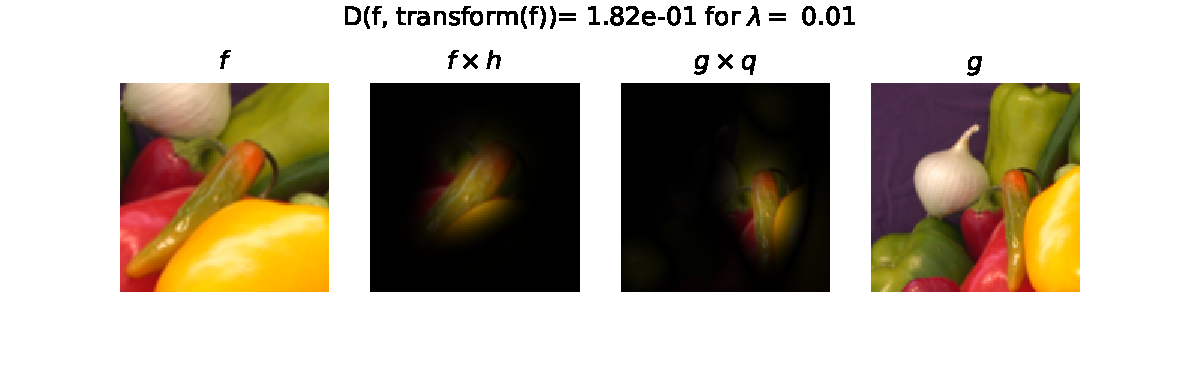
\includegraphics[width=\textwidth]{ch1-diffy/figures/fig_peppers/appendix_match_0.01_14.pdf}
%    \end{subfigure}
%    \begin{subfigure}{0.60\textwidth}
%    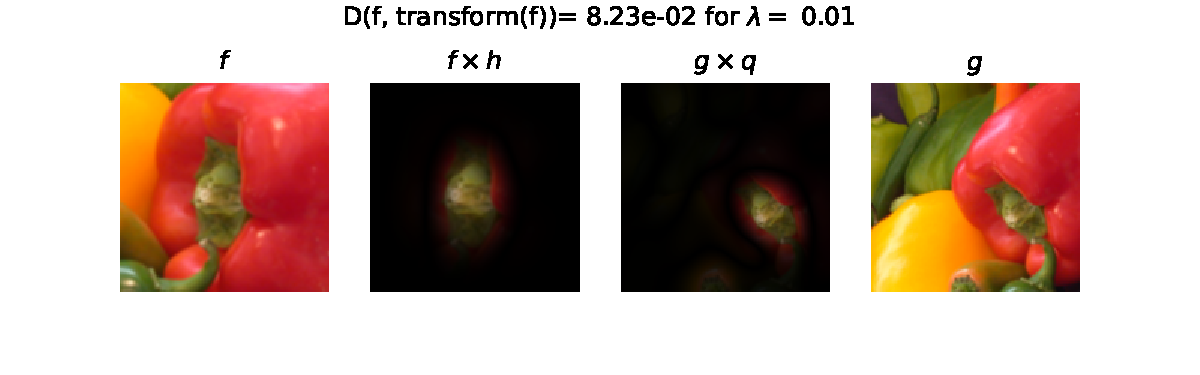
\includegraphics[width=\textwidth]{ch1-diffy/figures/fig_peppers/appendix_match_0.01_19.pdf}
%    \end{subfigure}
%    \begin{subfigure}{0.60\textwidth}
%    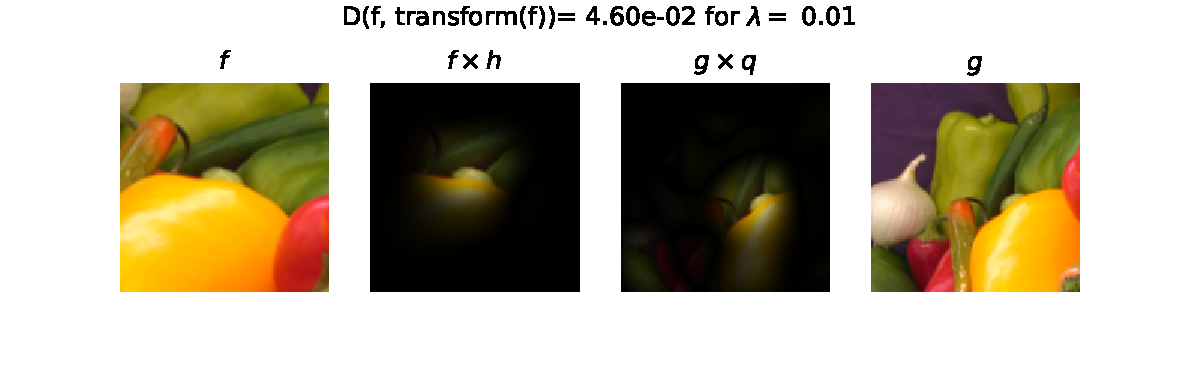
\includegraphics[width=\textwidth]{ch1-diffy/figures/fig_peppers/appendix_match_0.01_8.pdf}
%    \end{subfigure}
%    \begin{subfigure}{0.60\textwidth}
%    \includegraphics[width=\textwidth]{ch1-diffy/figures/fig_peppers/appendix_match_0.01_9.pdf}
%    \end{subfigure}
%    \begin{subfigure}{0.60\textwidth}
%    \includegraphics[width=\textwidth]{ch1-diffy/figures/fig_peppers/appendix_match_0.01_15.pdf}
%    \end{subfigure}
%    \begin{subfigure}{0.60\textwidth}
%    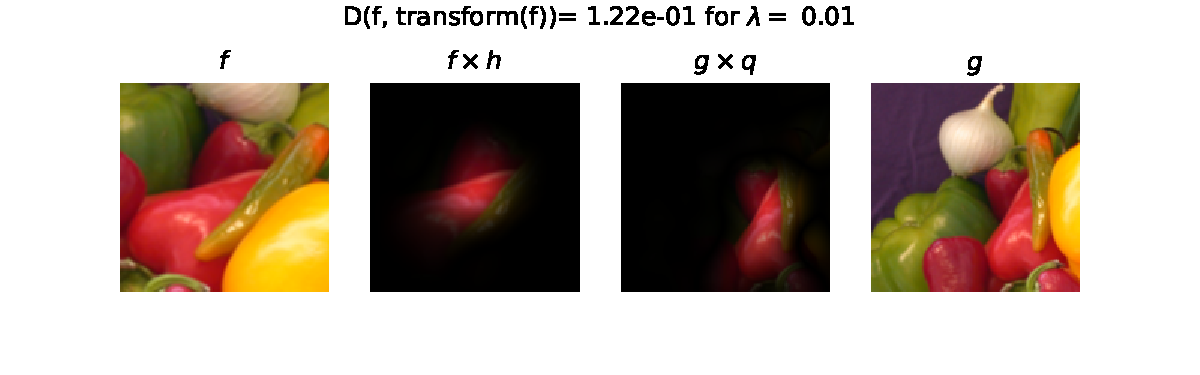
\includegraphics[width=\textwidth]{ch1-diffy/figures/fig_peppers/appendix_match_0.01_5.pdf}
%    \end{subfigure}
%    \caption{$\widehat D_\lambda(f, \textrm{transform}(f))$ for $f$ random patches from \texttt{peppers}. We show $f$, $g=\textrm{transform}(f)$ as well as the optimal functions $h$ and $q$.}
%    \label{fig:appendix-peppers-matching}
%\end{figure}


\section{Warping demonstrations}\label{sec:appendix-warping}
The warps below were generated using file \texttt{appendix\char`_warp.py} in our source code, using an image from ImageNet. Rows are from different samples, columns for different warp temperatures. All waps use $c=2$.

%todo : hidden for compilation speed
%\begin{figure}[!h]
%    \centering
%    \begin{subfigure}{0.18\textwidth}
%    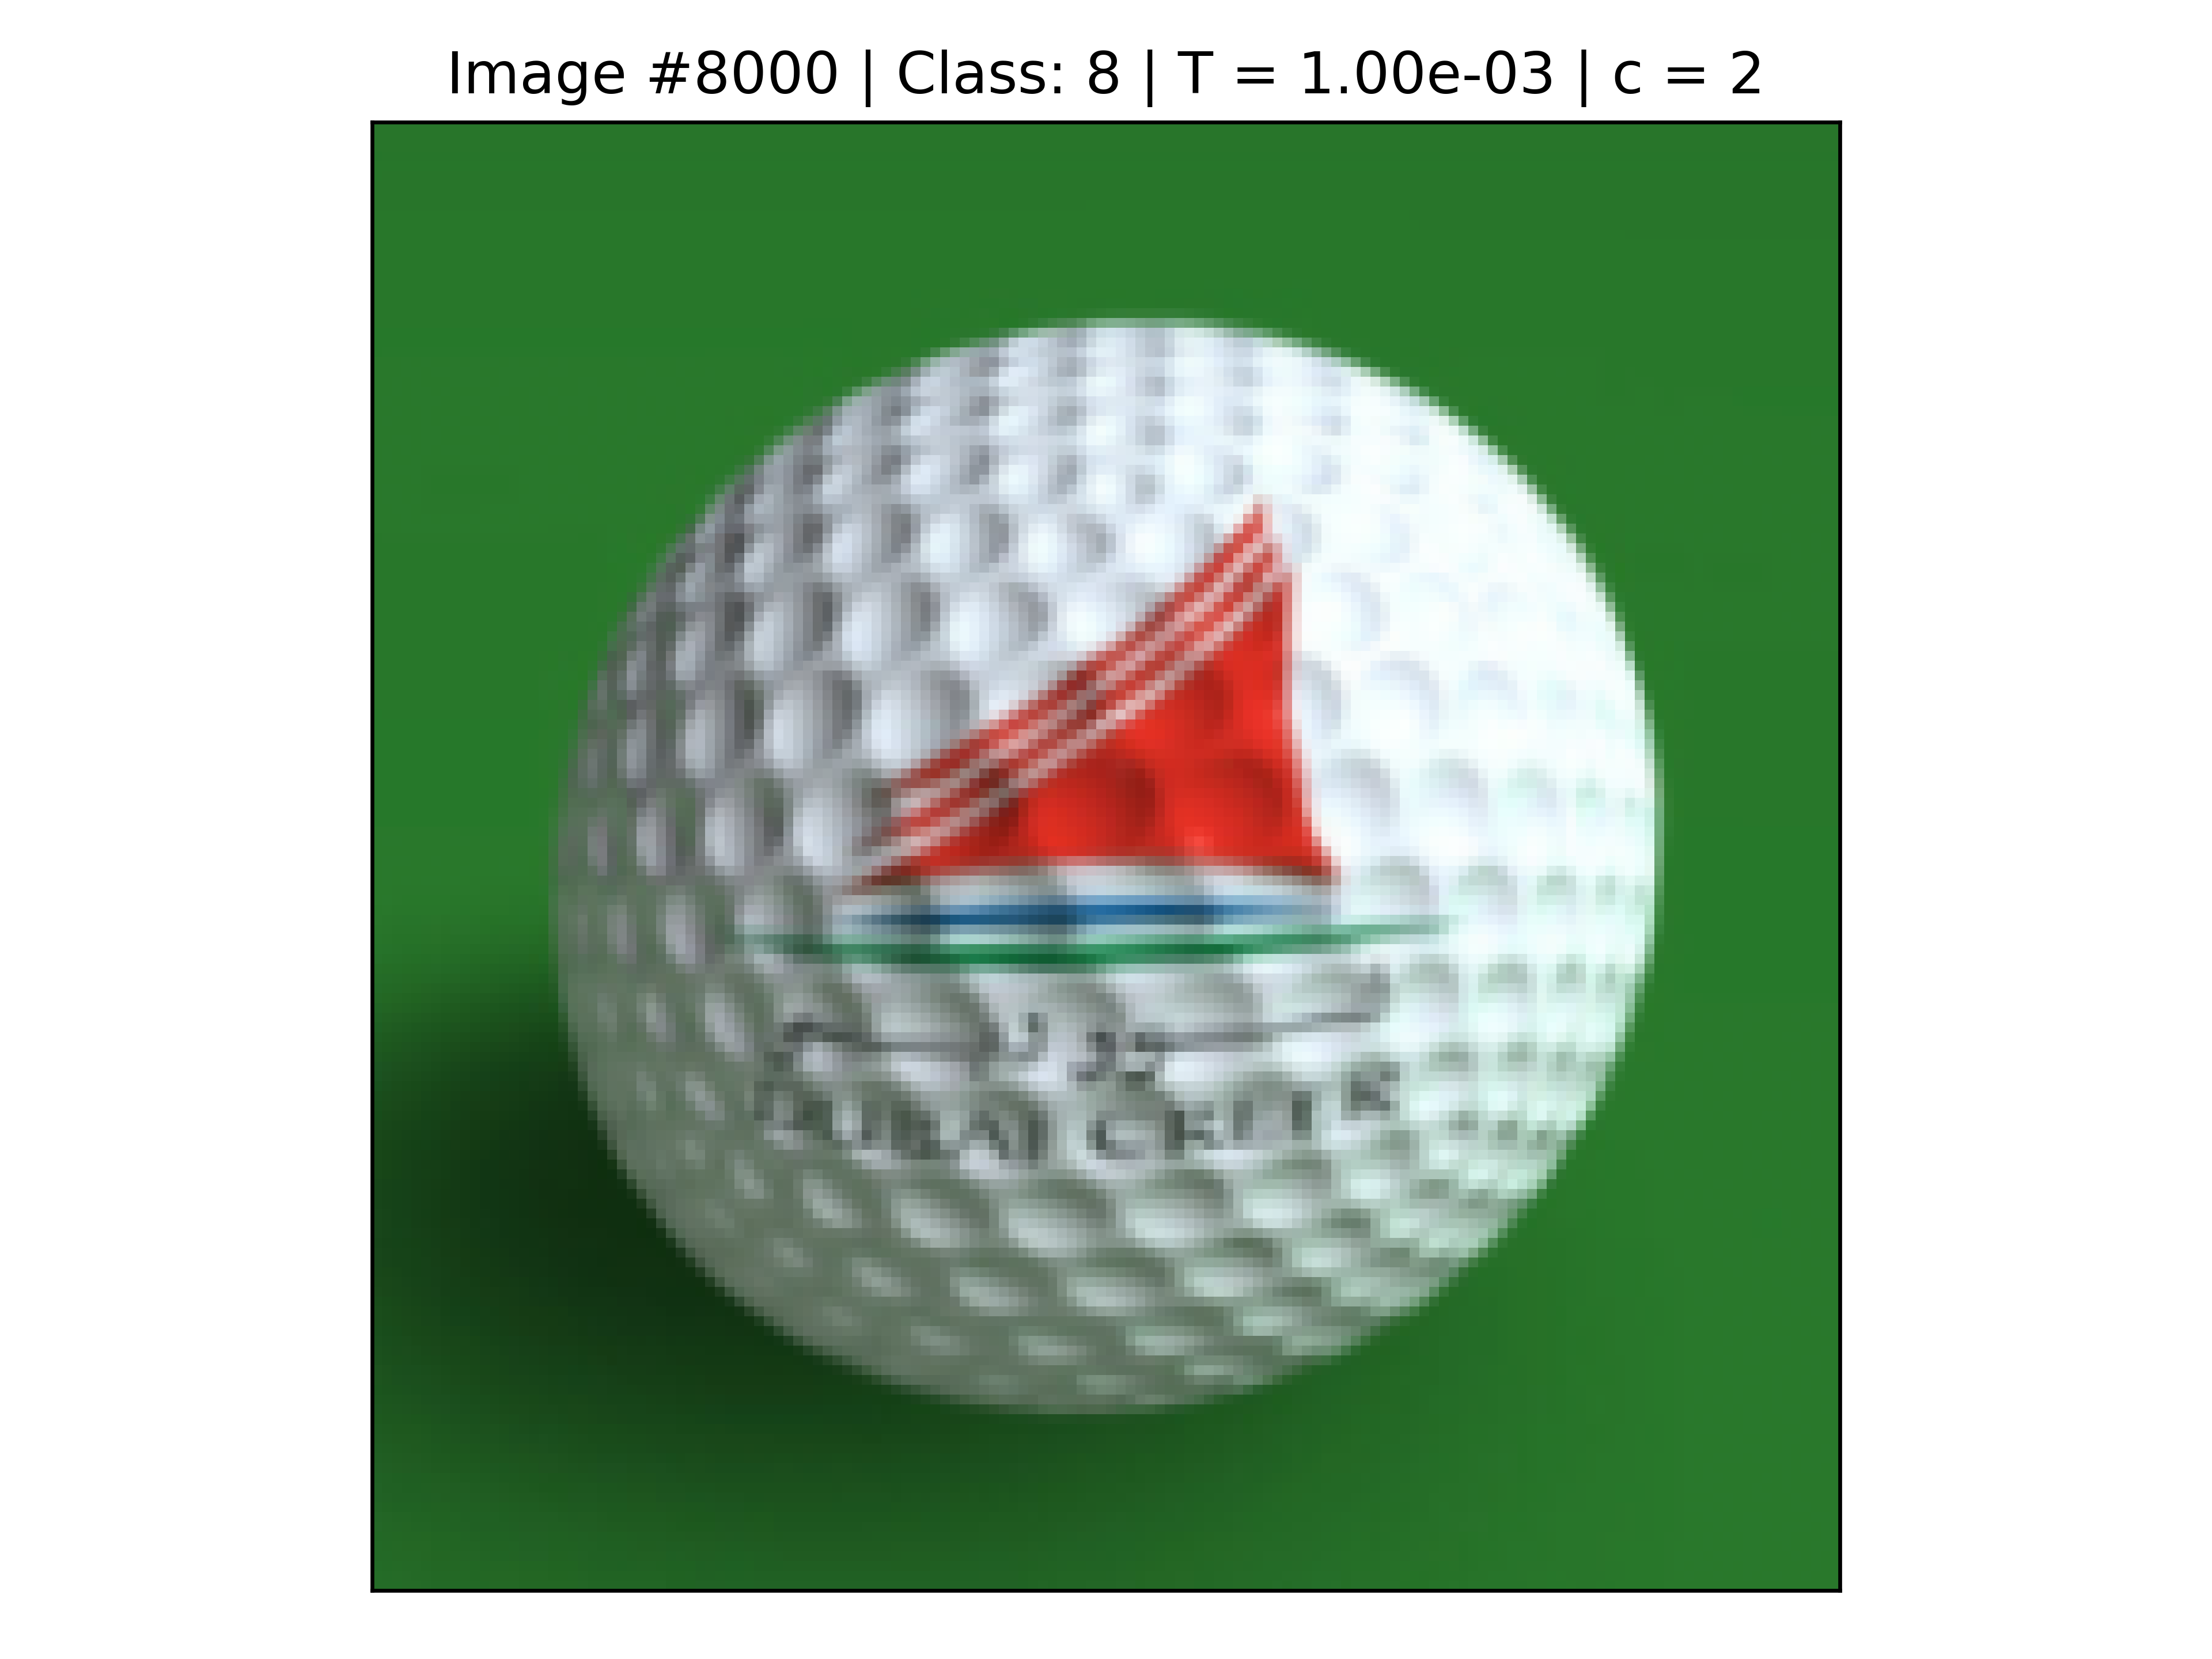
\includegraphics[width=\textwidth]{ch1-diffy/figures/warping_examples/8000_3_0.png}
%    \caption{$T=10^{-3}$}
%    % \label{fig:my_label}
%    \end{subfigure}
%    \begin{subfigure}{0.18\textwidth}
%    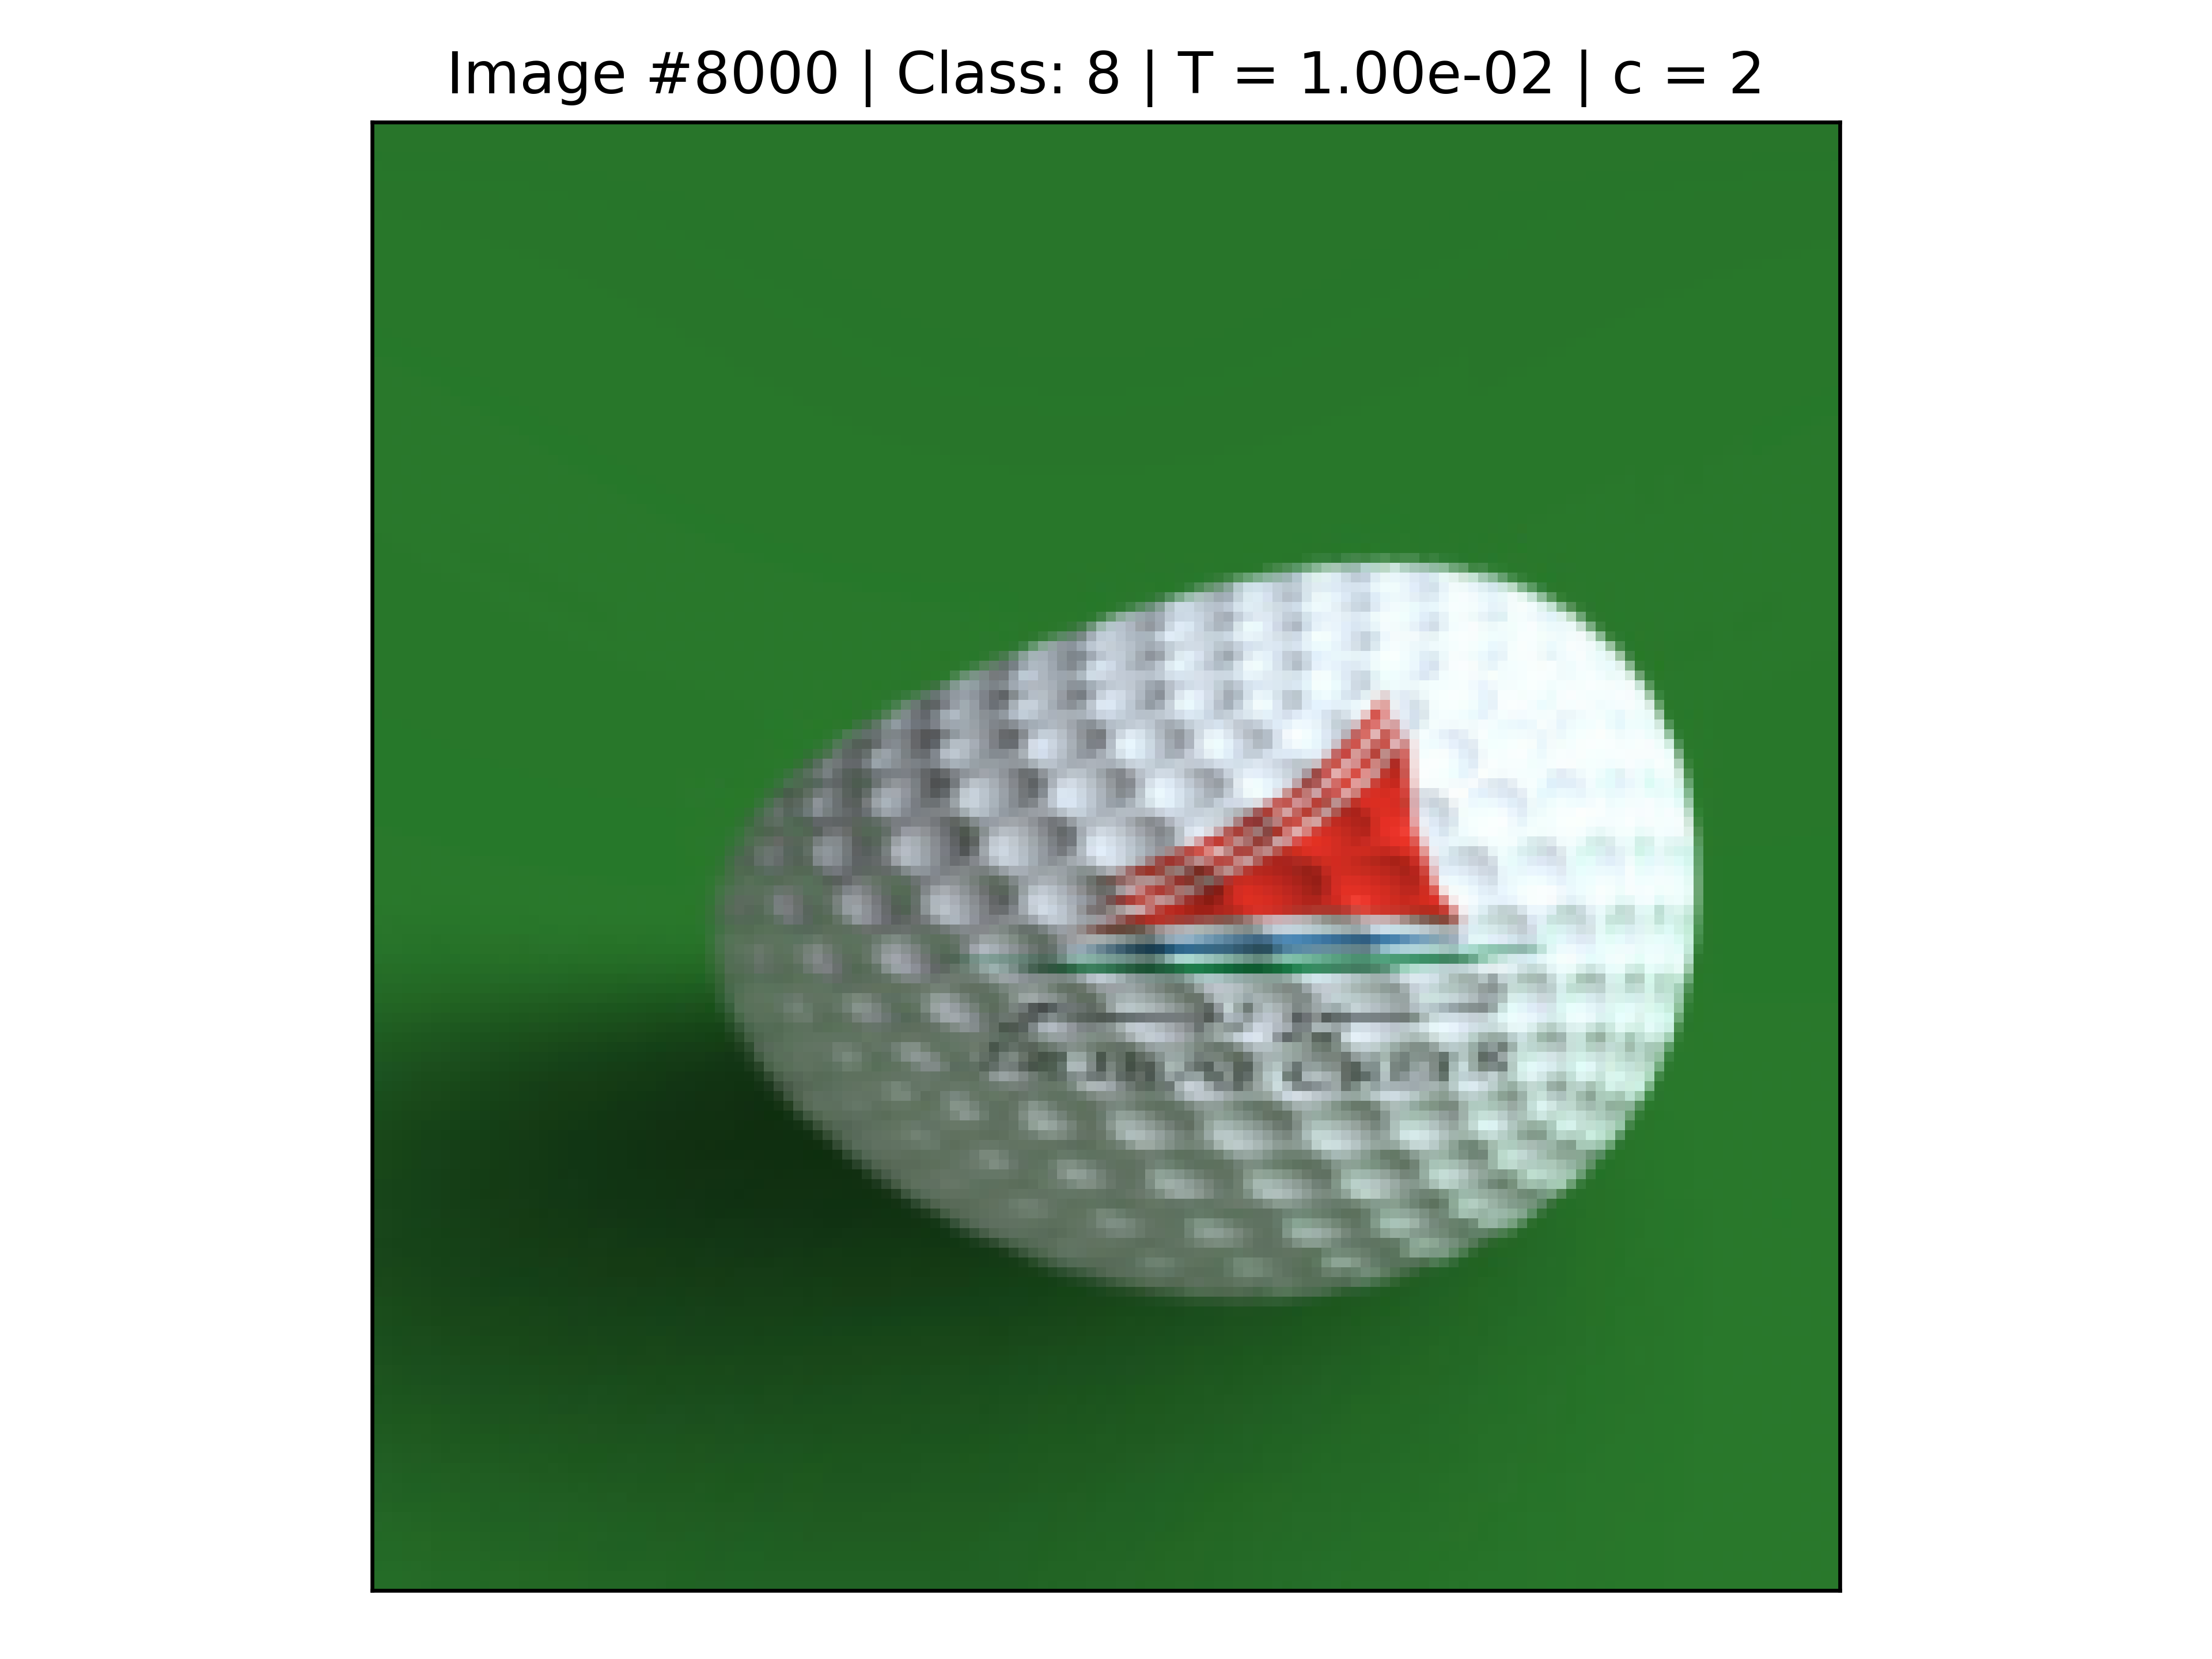
\includegraphics[width=\textwidth]{ch1-diffy/figures/warping_examples/8000_2_0.png}
%    \caption{$T=10^{-2}$}
%    % \label{fig:my_label}
%    \end{subfigure}
%    \begin{subfigure}{0.18\textwidth}
%    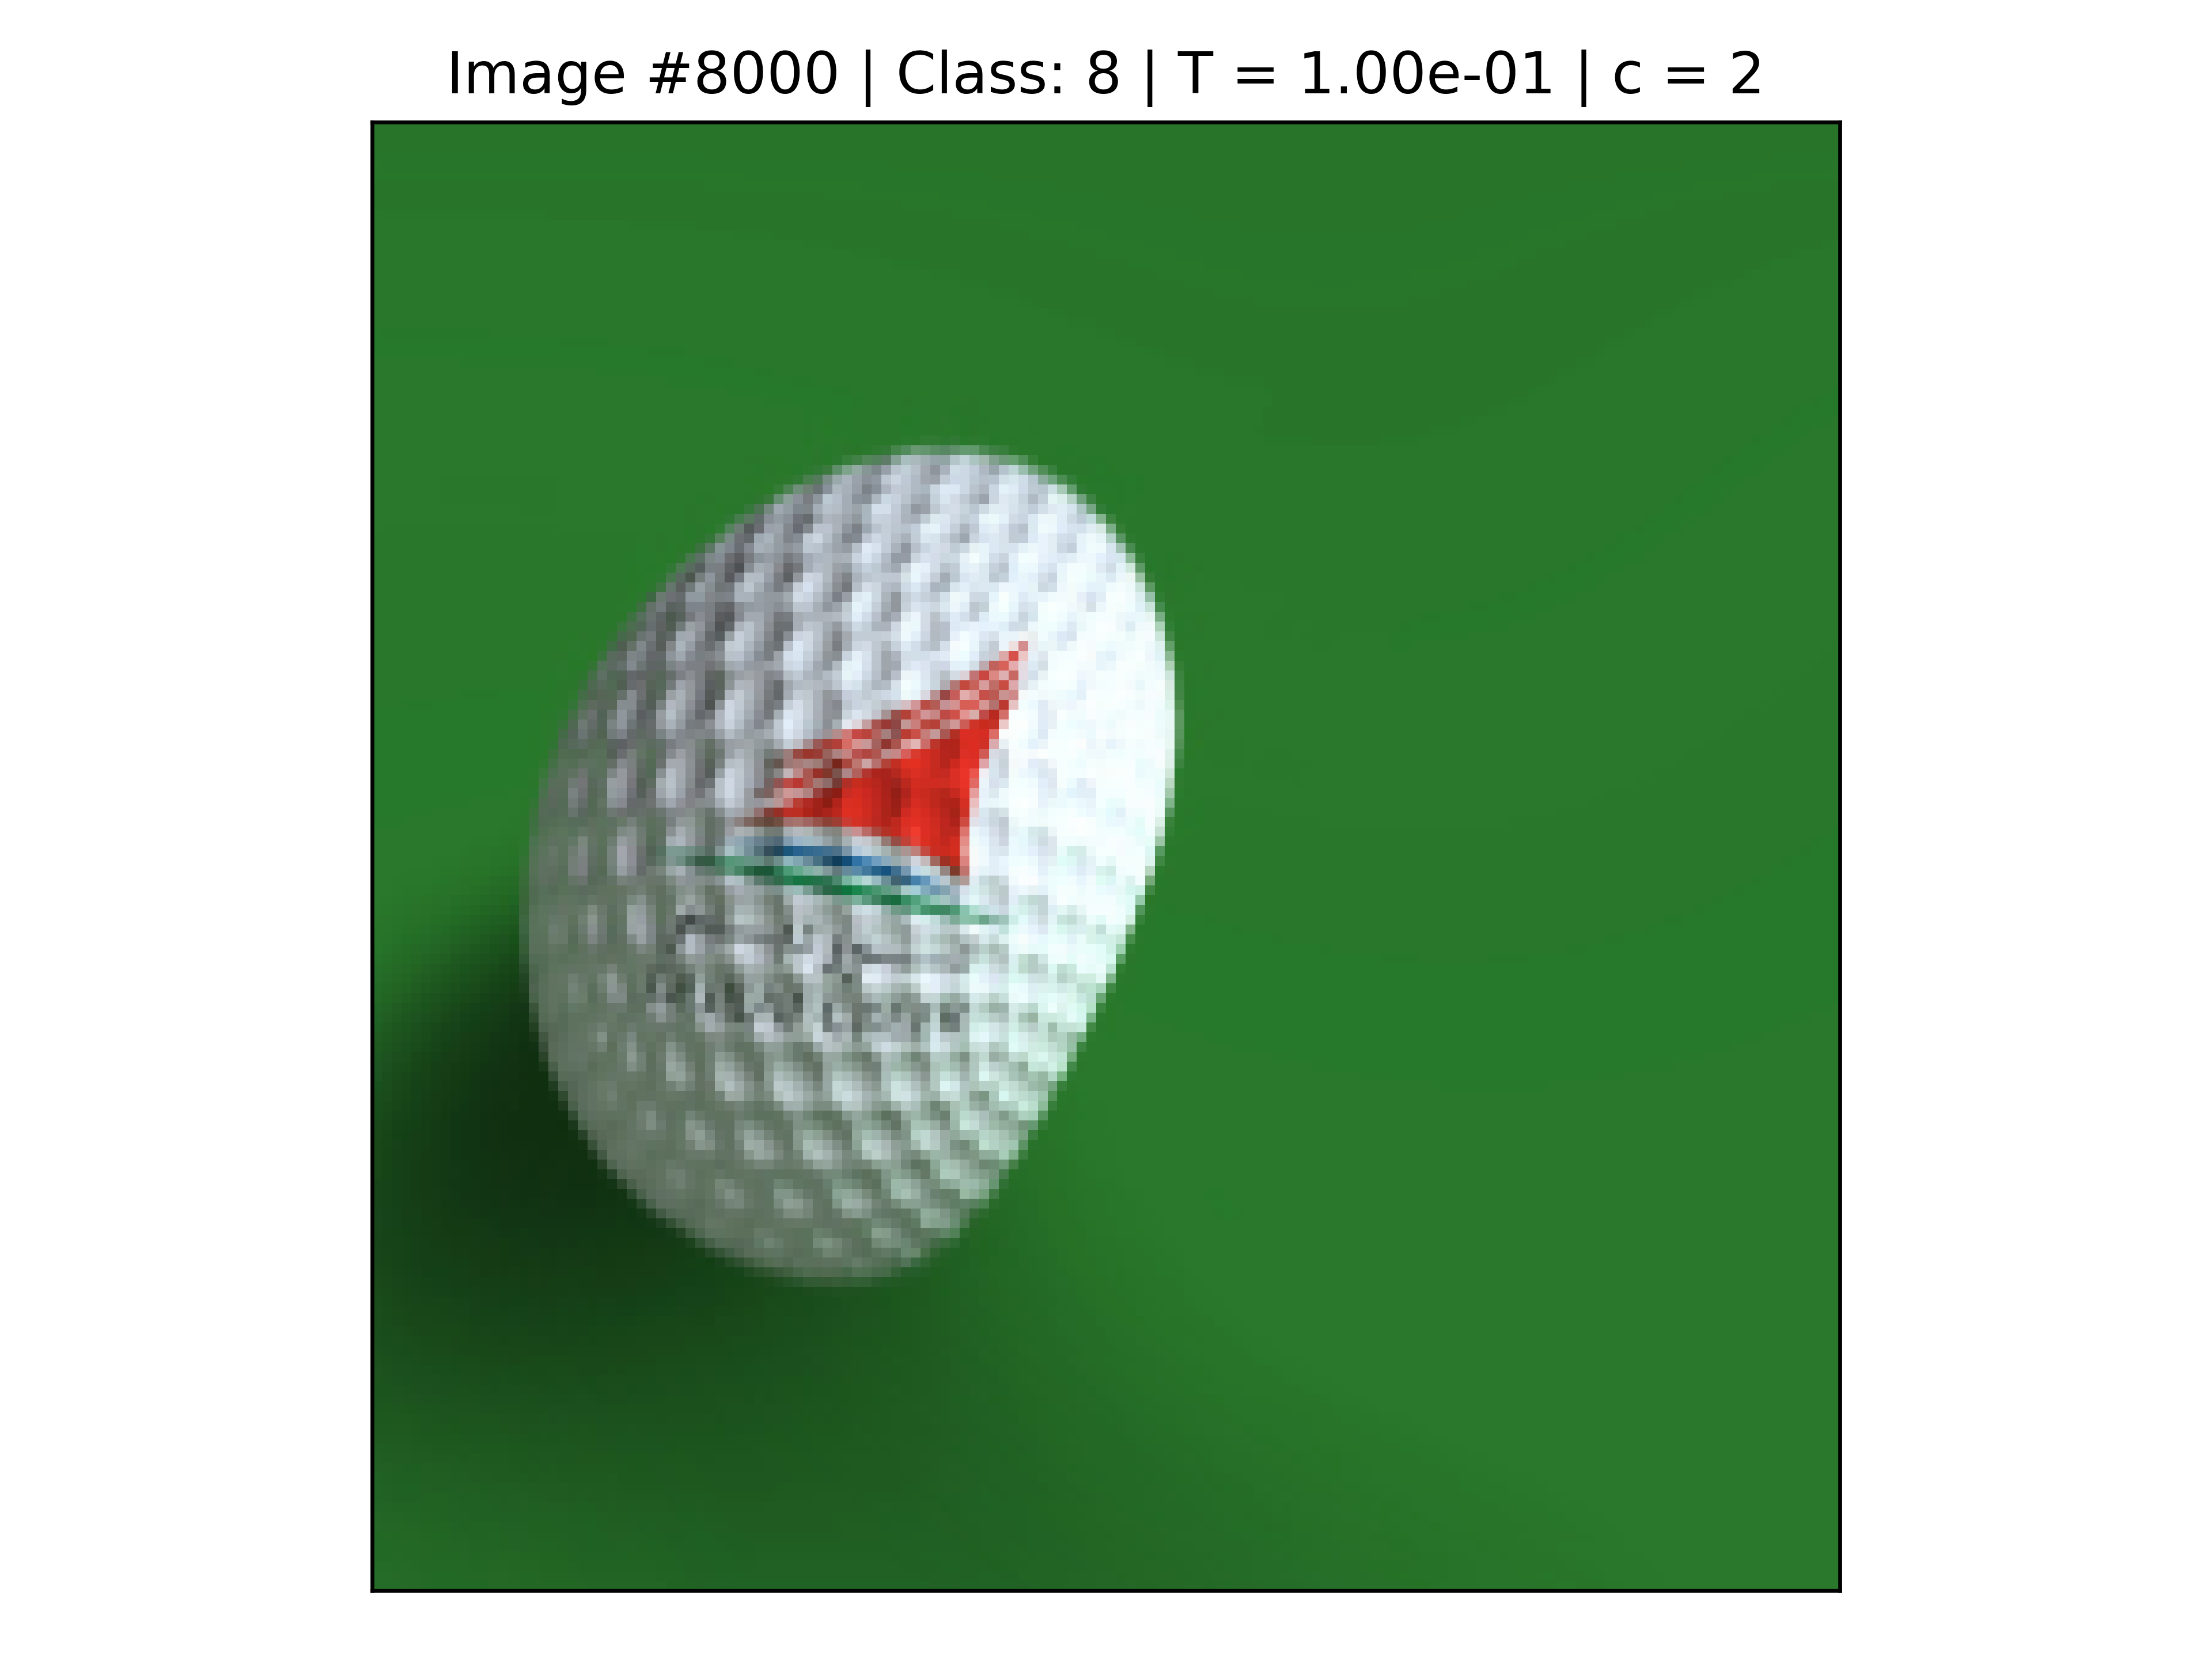
\includegraphics[width=\textwidth]{ch1-diffy/figures/warping_examples/8000_1_0.png}
%    \caption{$T=10^{-1}$}
%    % \label{fig:my_label}
%    \end{subfigure}
%    \begin{subfigure}{0.18\textwidth}
%    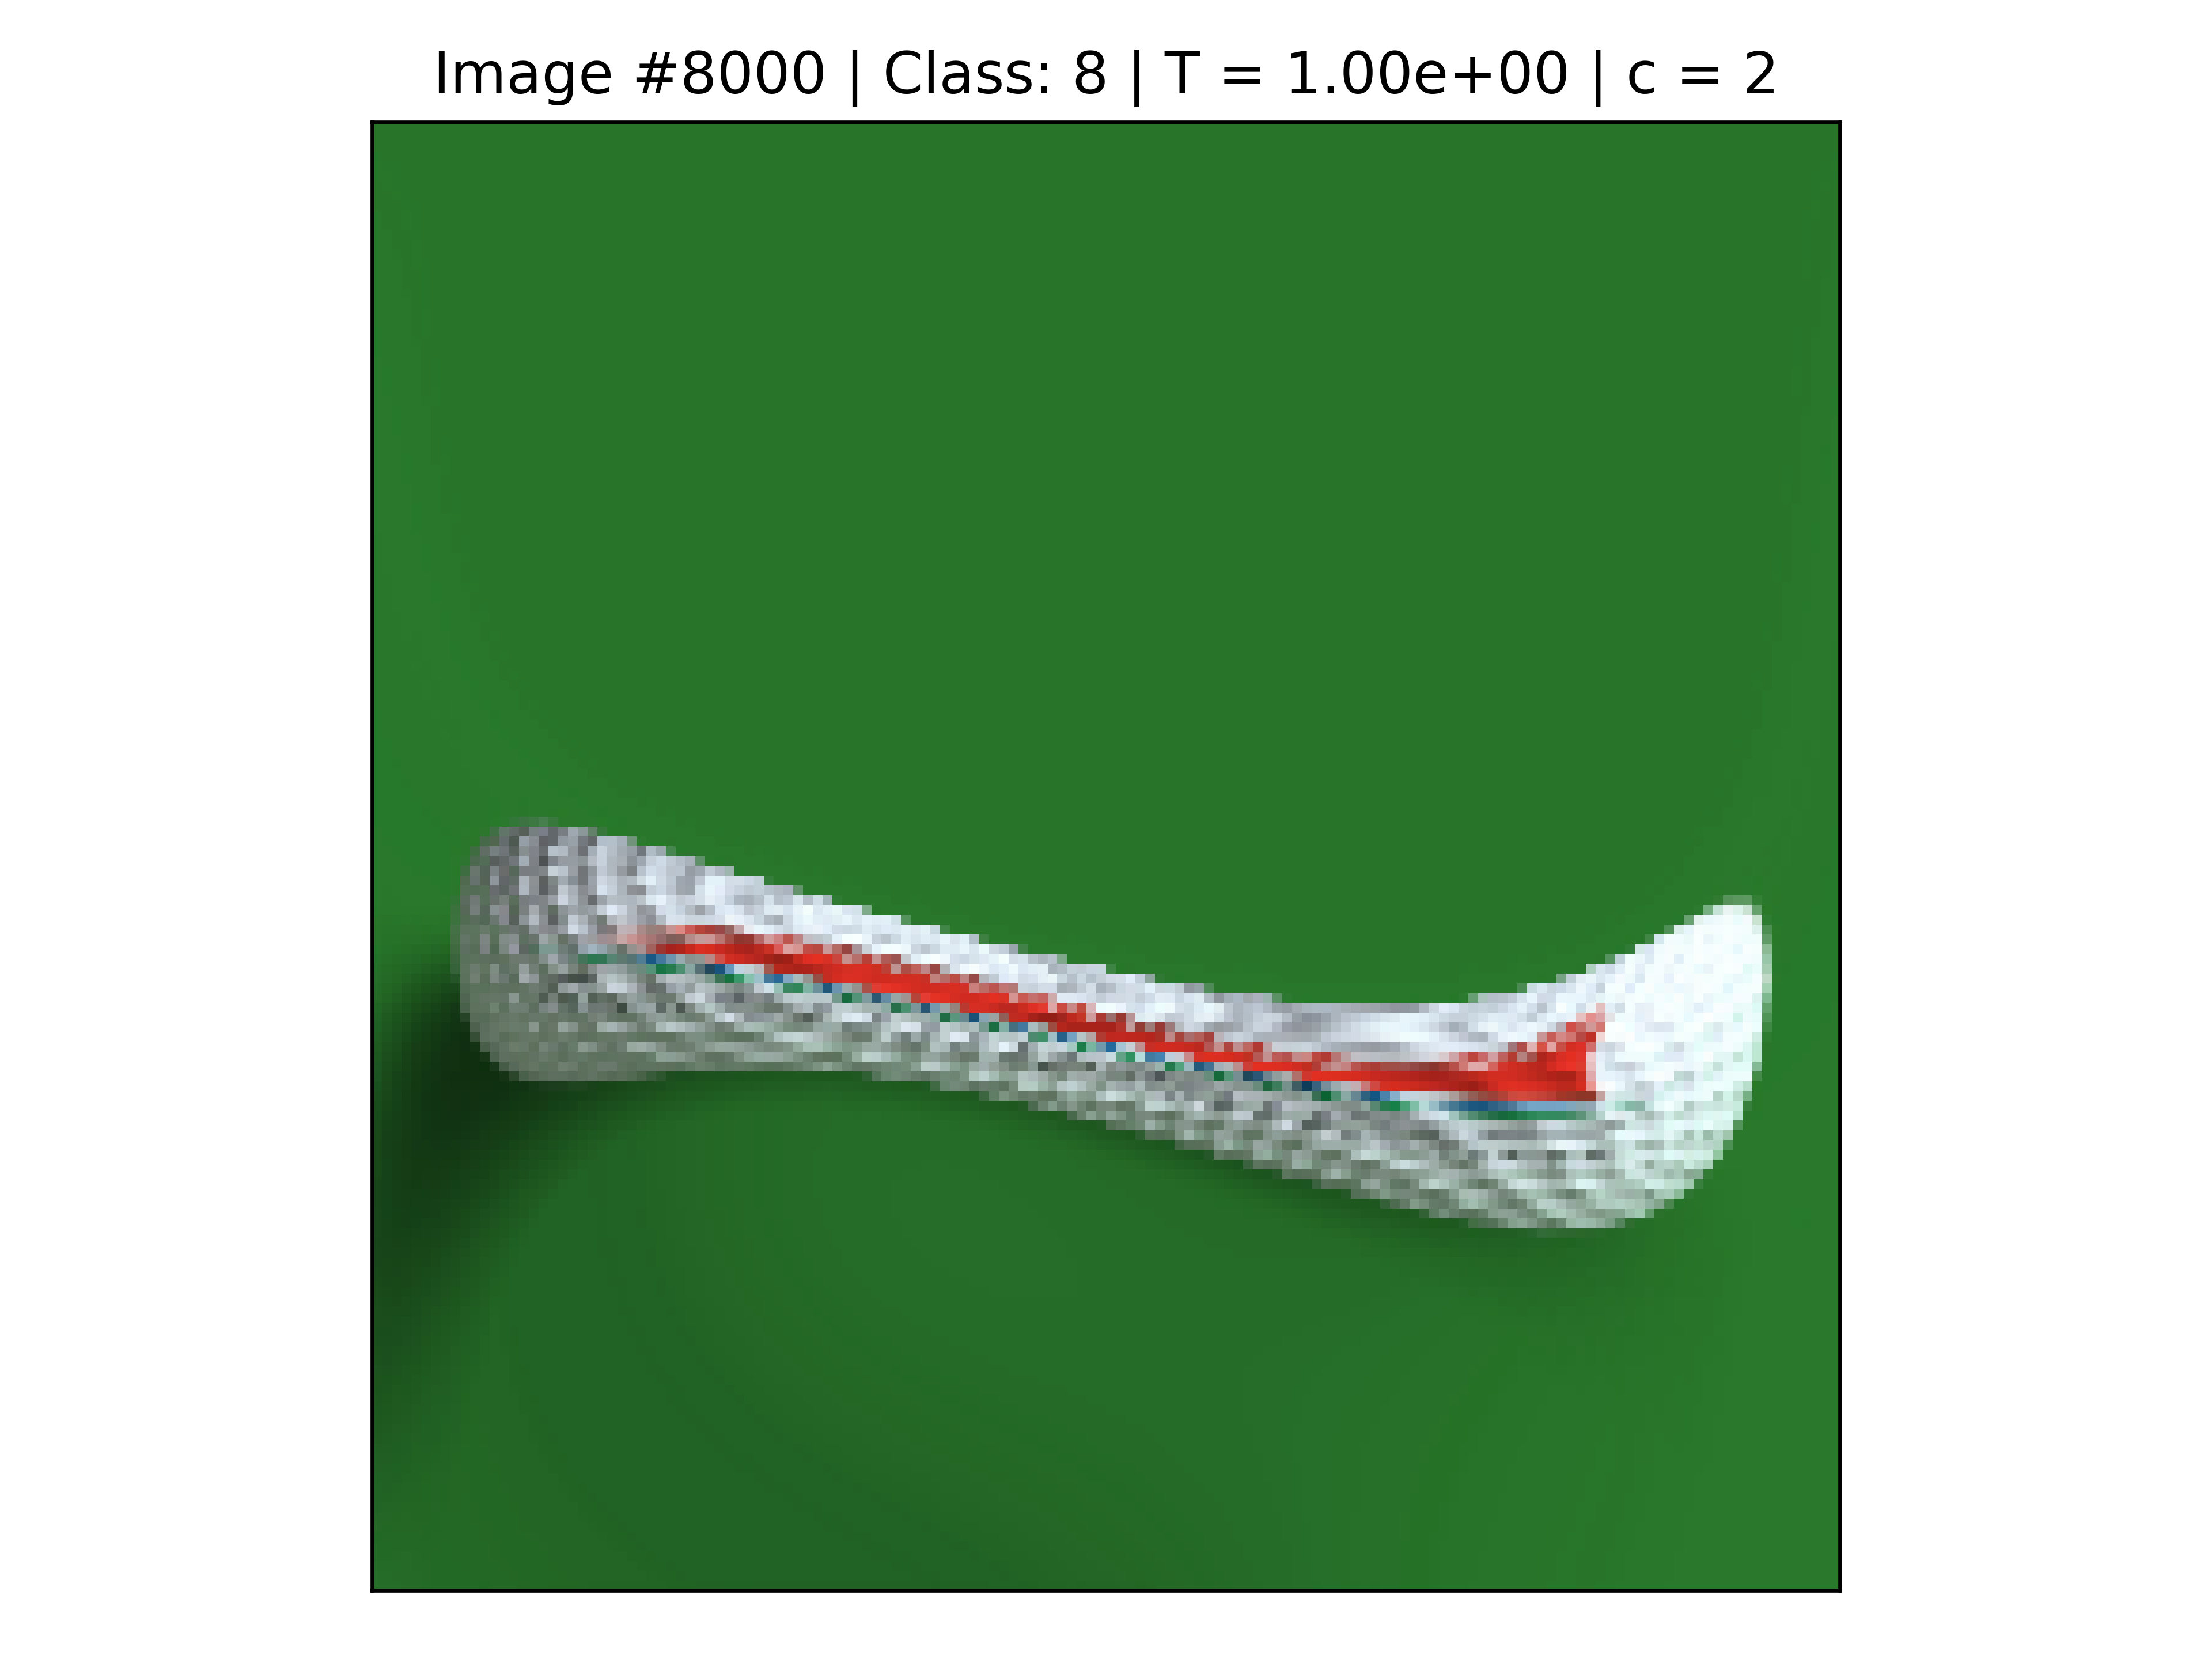
\includegraphics[width=\textwidth]{ch1-diffy/figures/warping_examples/8000_0_0.png}
%    \caption{$T=1$}
%    % \label{fig:my_label}
%    \end{subfigure}
%    \begin{subfigure}{0.18\textwidth}
%    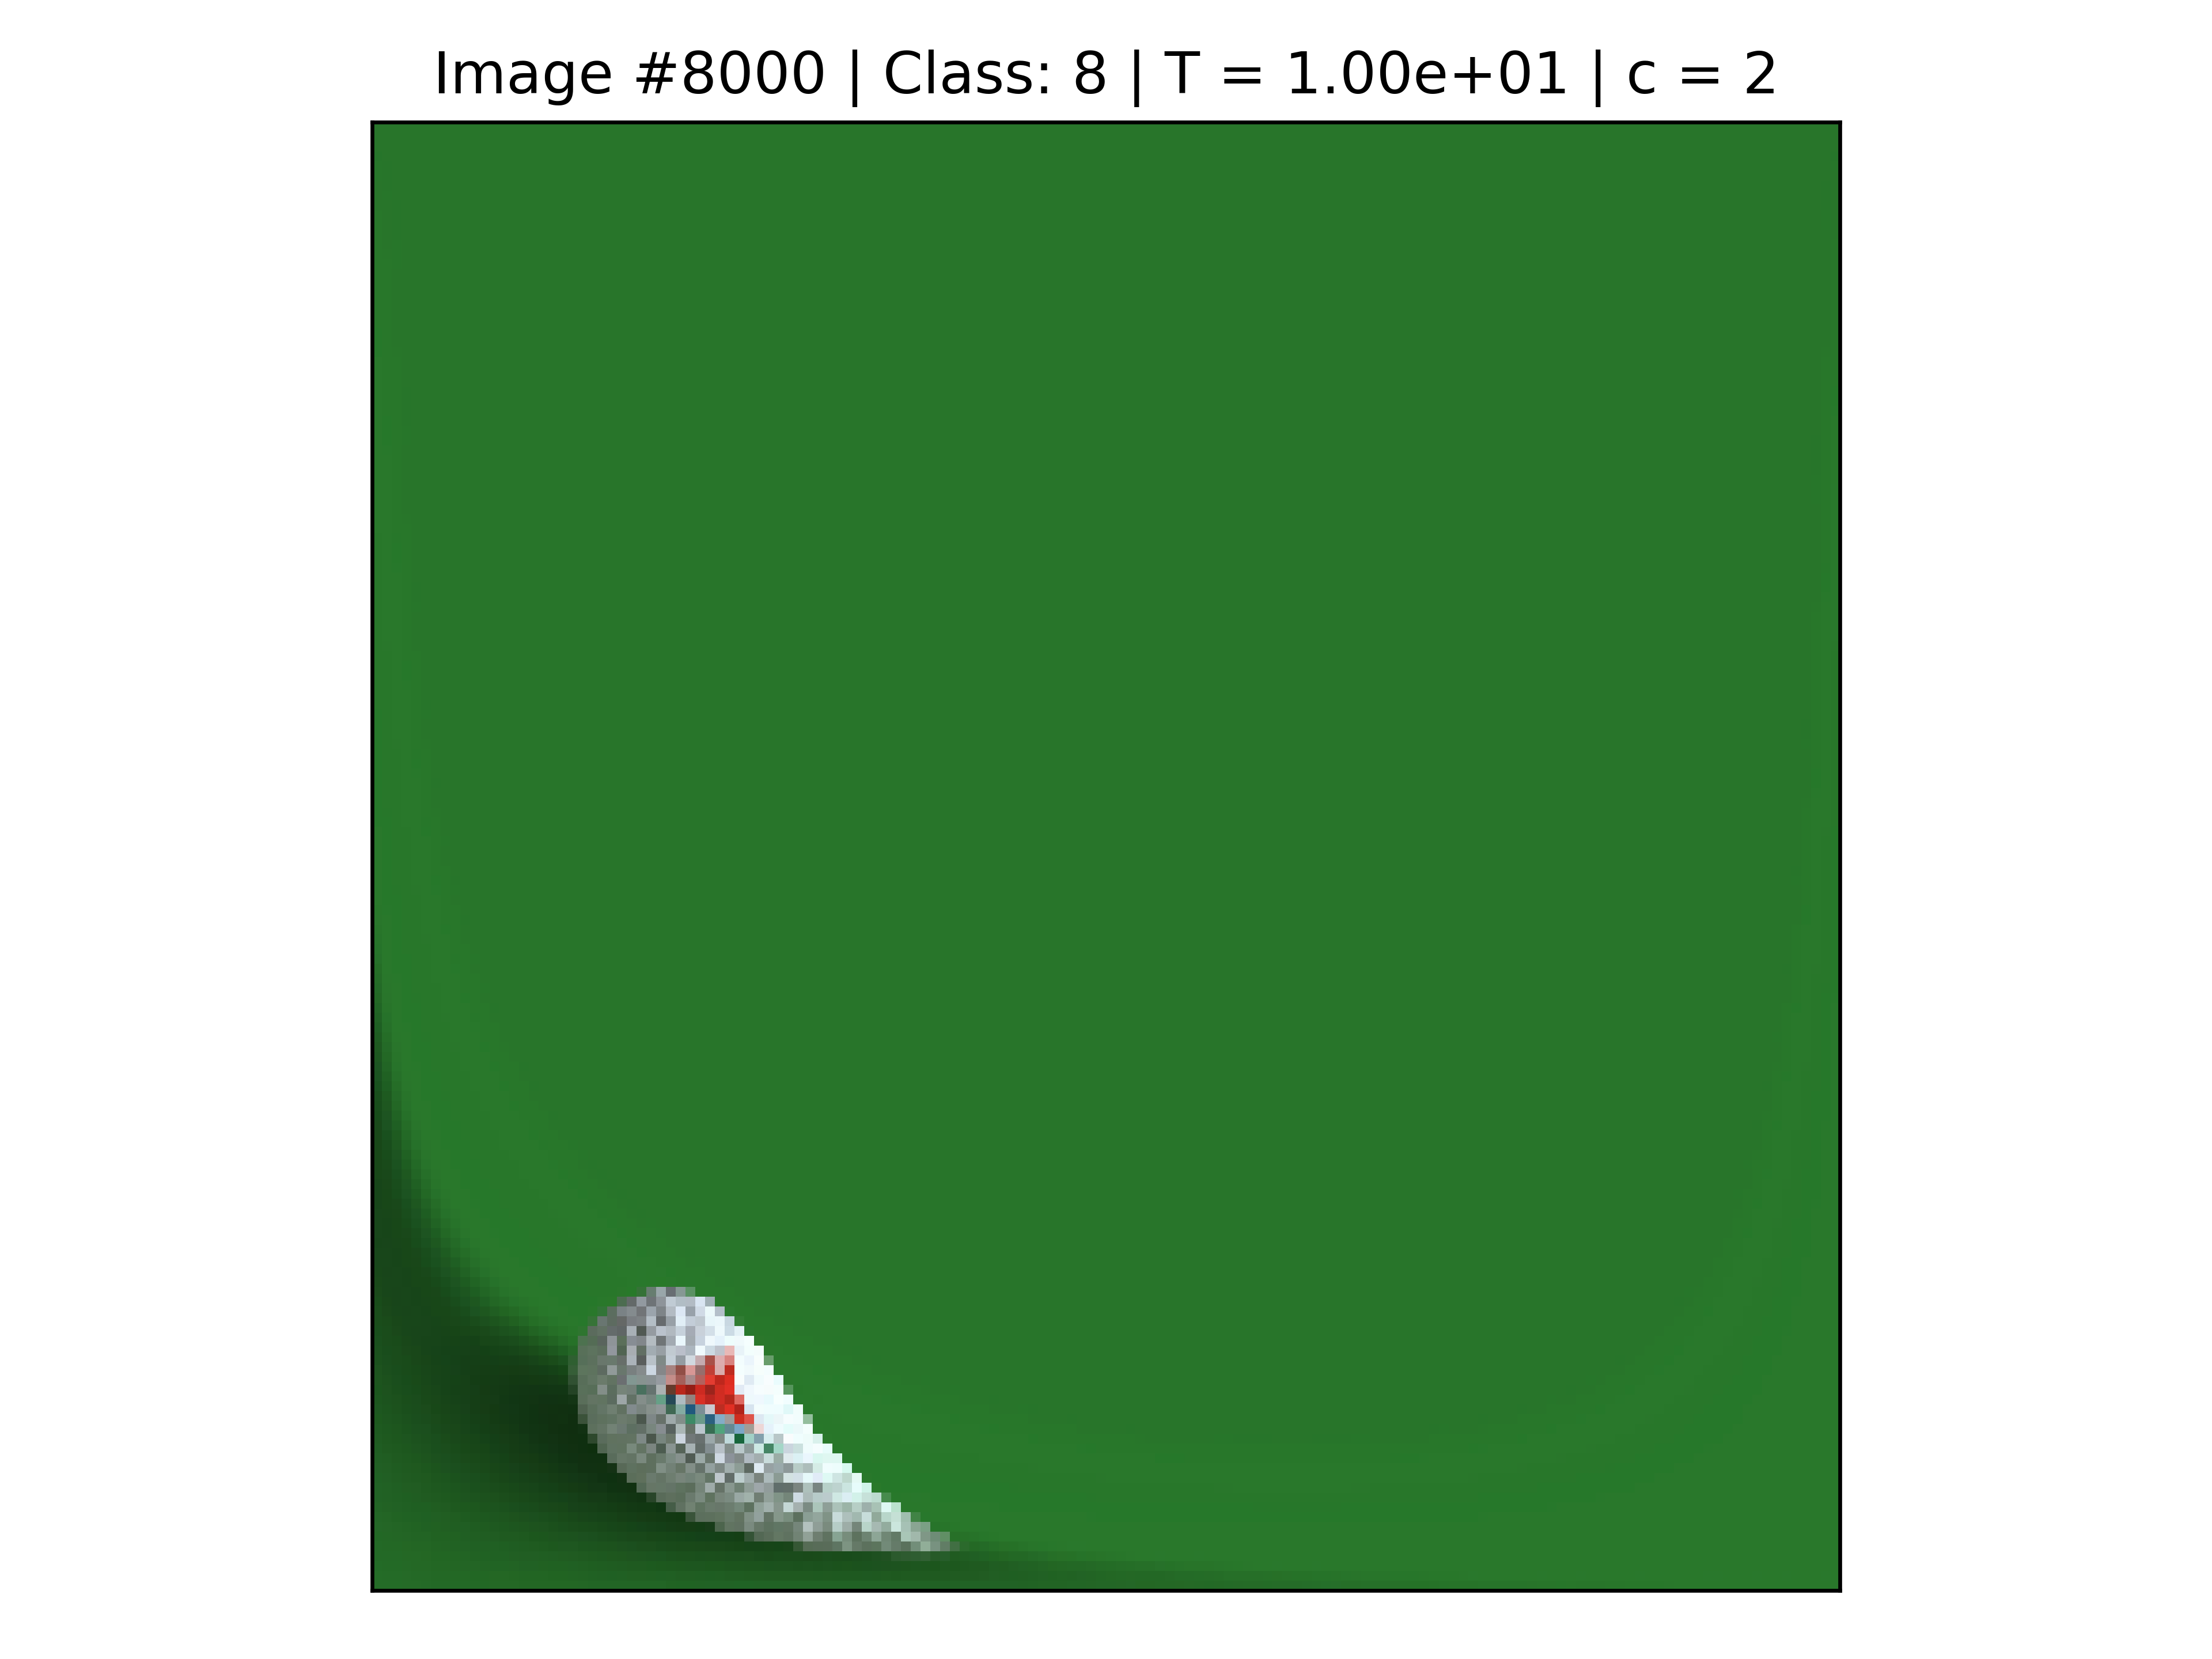
\includegraphics[width=\textwidth]{ch1-diffy/figures/warping_examples/8000_-1_0.png}
%    \caption{$T=10$}
%    % \label{fig:my_label}
%    \end{subfigure}
%    %%%%%
%    \begin{subfigure}{0.18\textwidth}
%    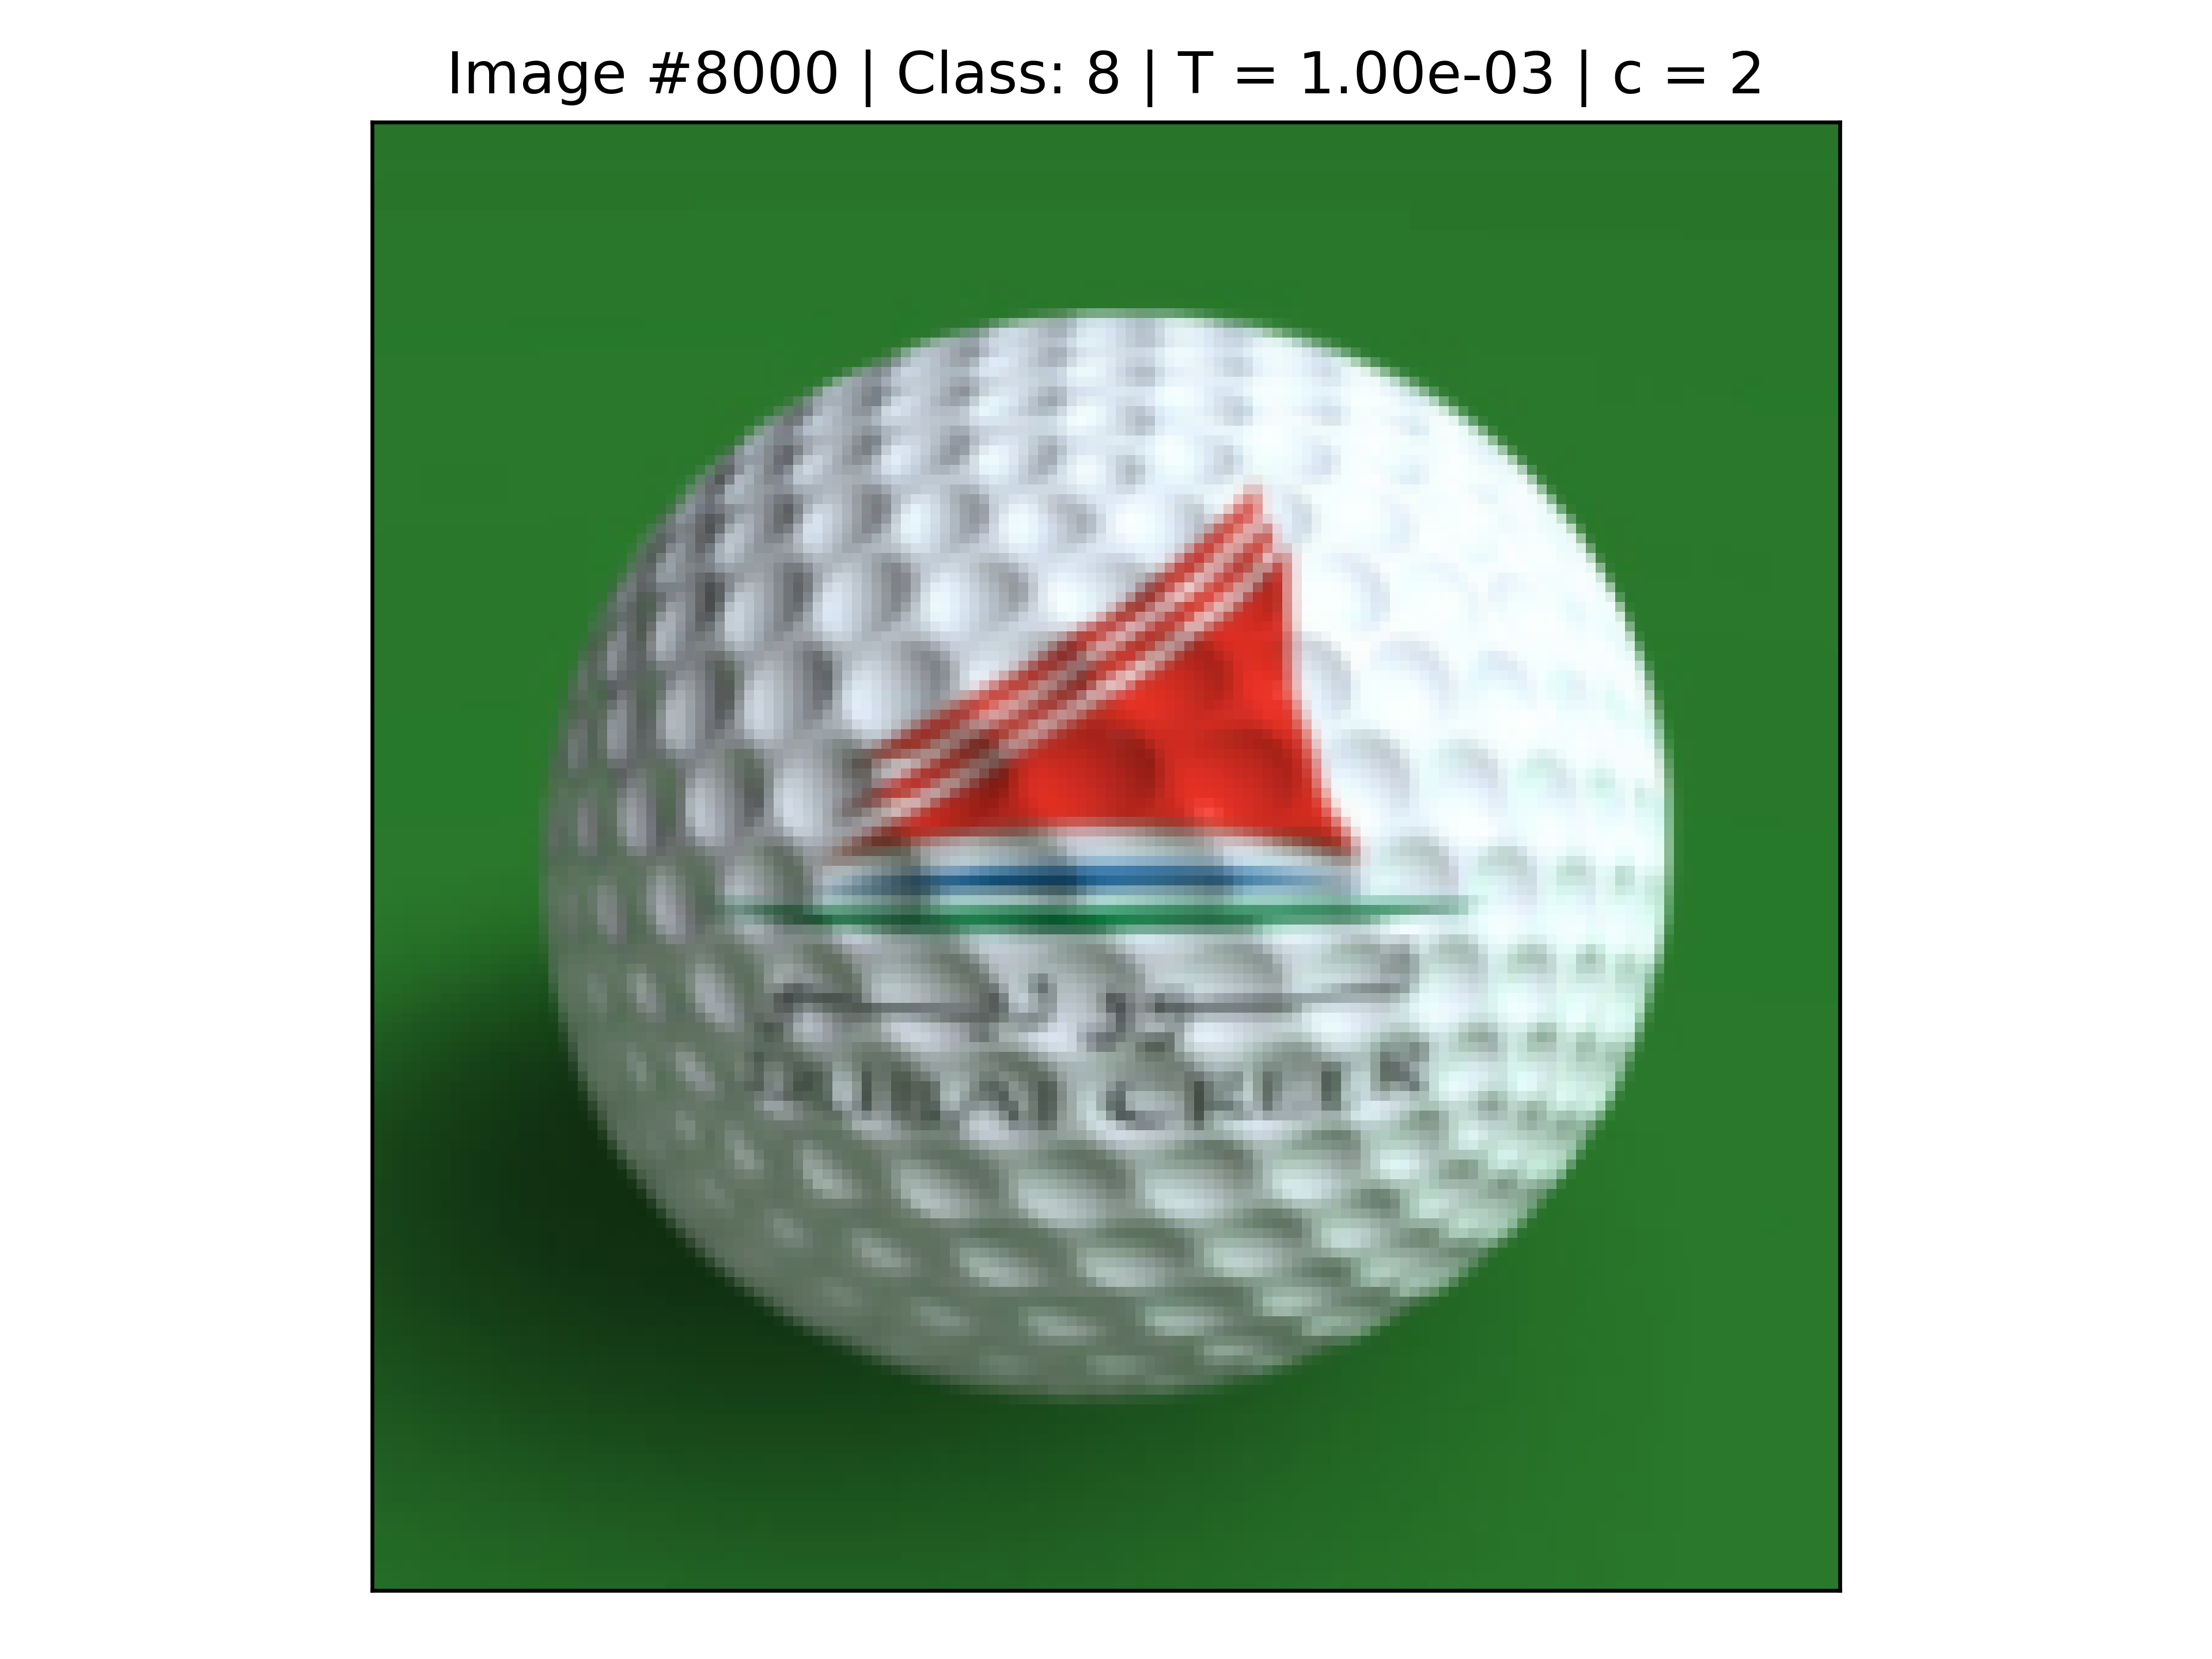
\includegraphics[width=\textwidth]{ch1-diffy/figures/warping_examples/8000_3_1.png}
%    \caption{$T=10^{-3}$}
%    % \label{fig:my_label}
%    \end{subfigure}
%    \begin{subfigure}{0.18\textwidth}
%    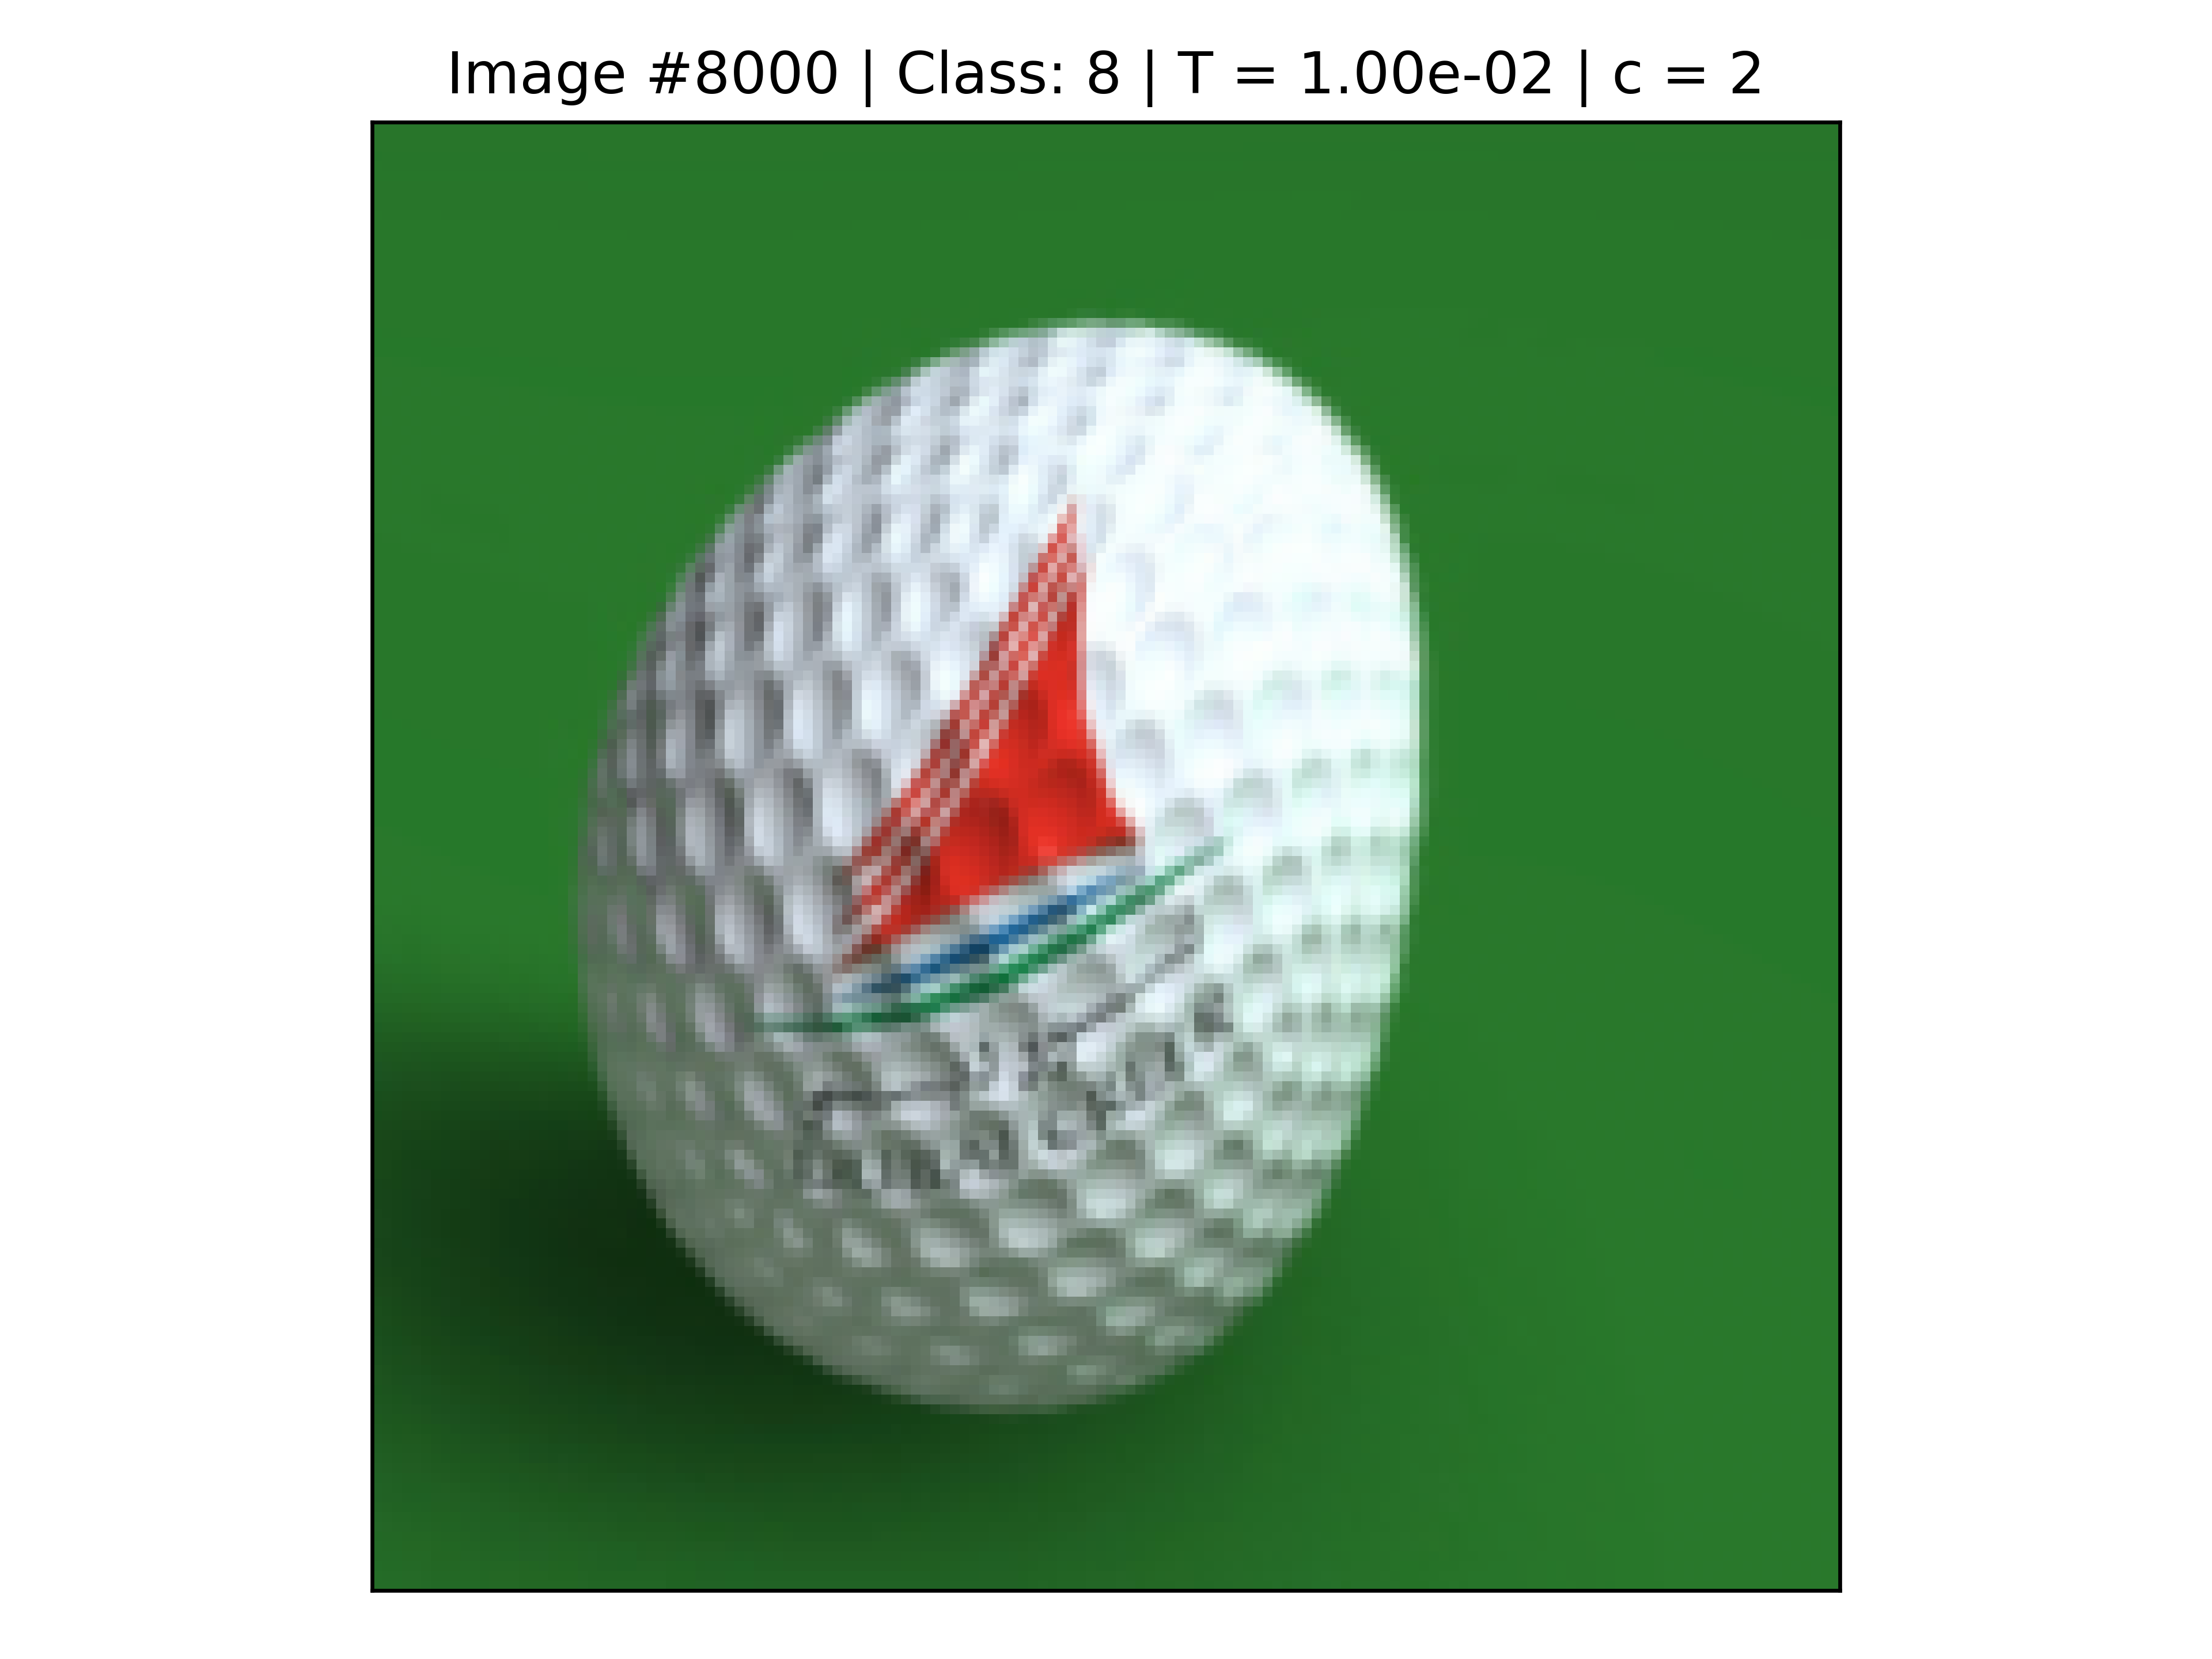
\includegraphics[width=\textwidth]{ch1-diffy/figures/warping_examples/8000_2_1.png}
%    \caption{$T=10^{-2}$}
%    % \label{fig:my_label}
%    \end{subfigure}
%    \begin{subfigure}{0.18\textwidth}
%    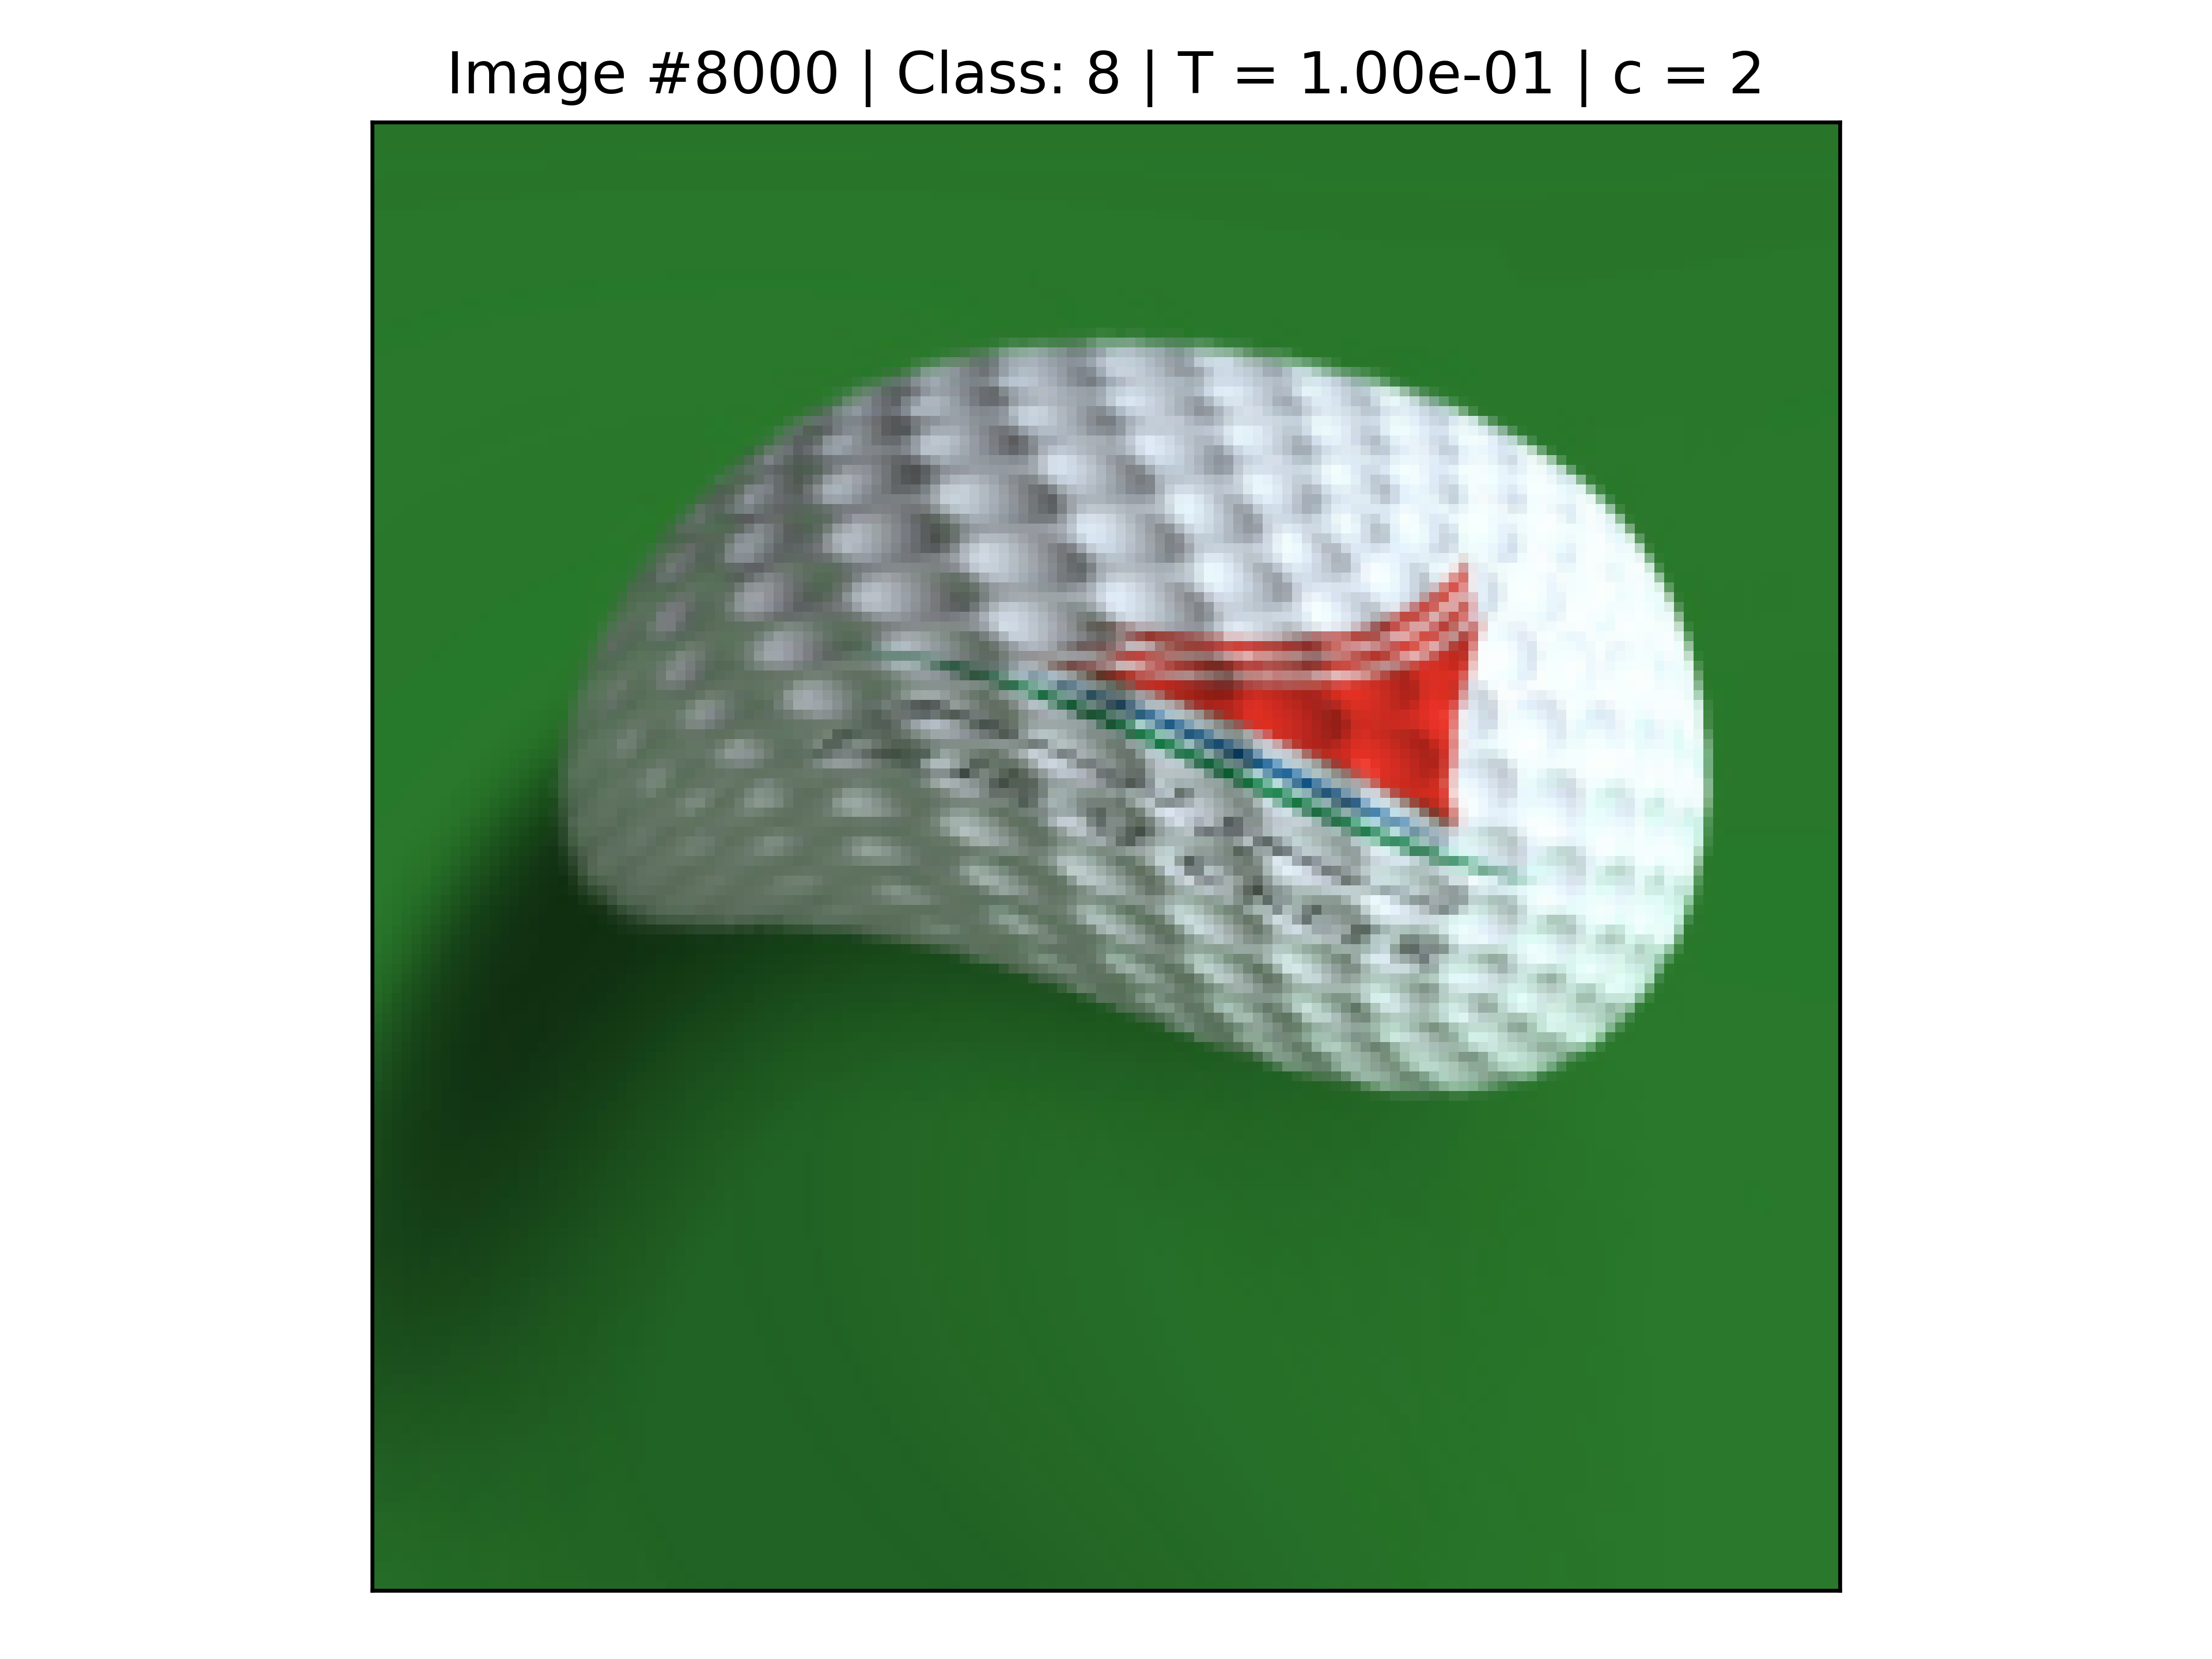
\includegraphics[width=\textwidth]{ch1-diffy/figures/warping_examples/8000_1_1.png}
%    \caption{$T=10^{-1}$}
%    % \label{fig:my_label}
%    \end{subfigure}
%    \begin{subfigure}{0.18\textwidth}
%    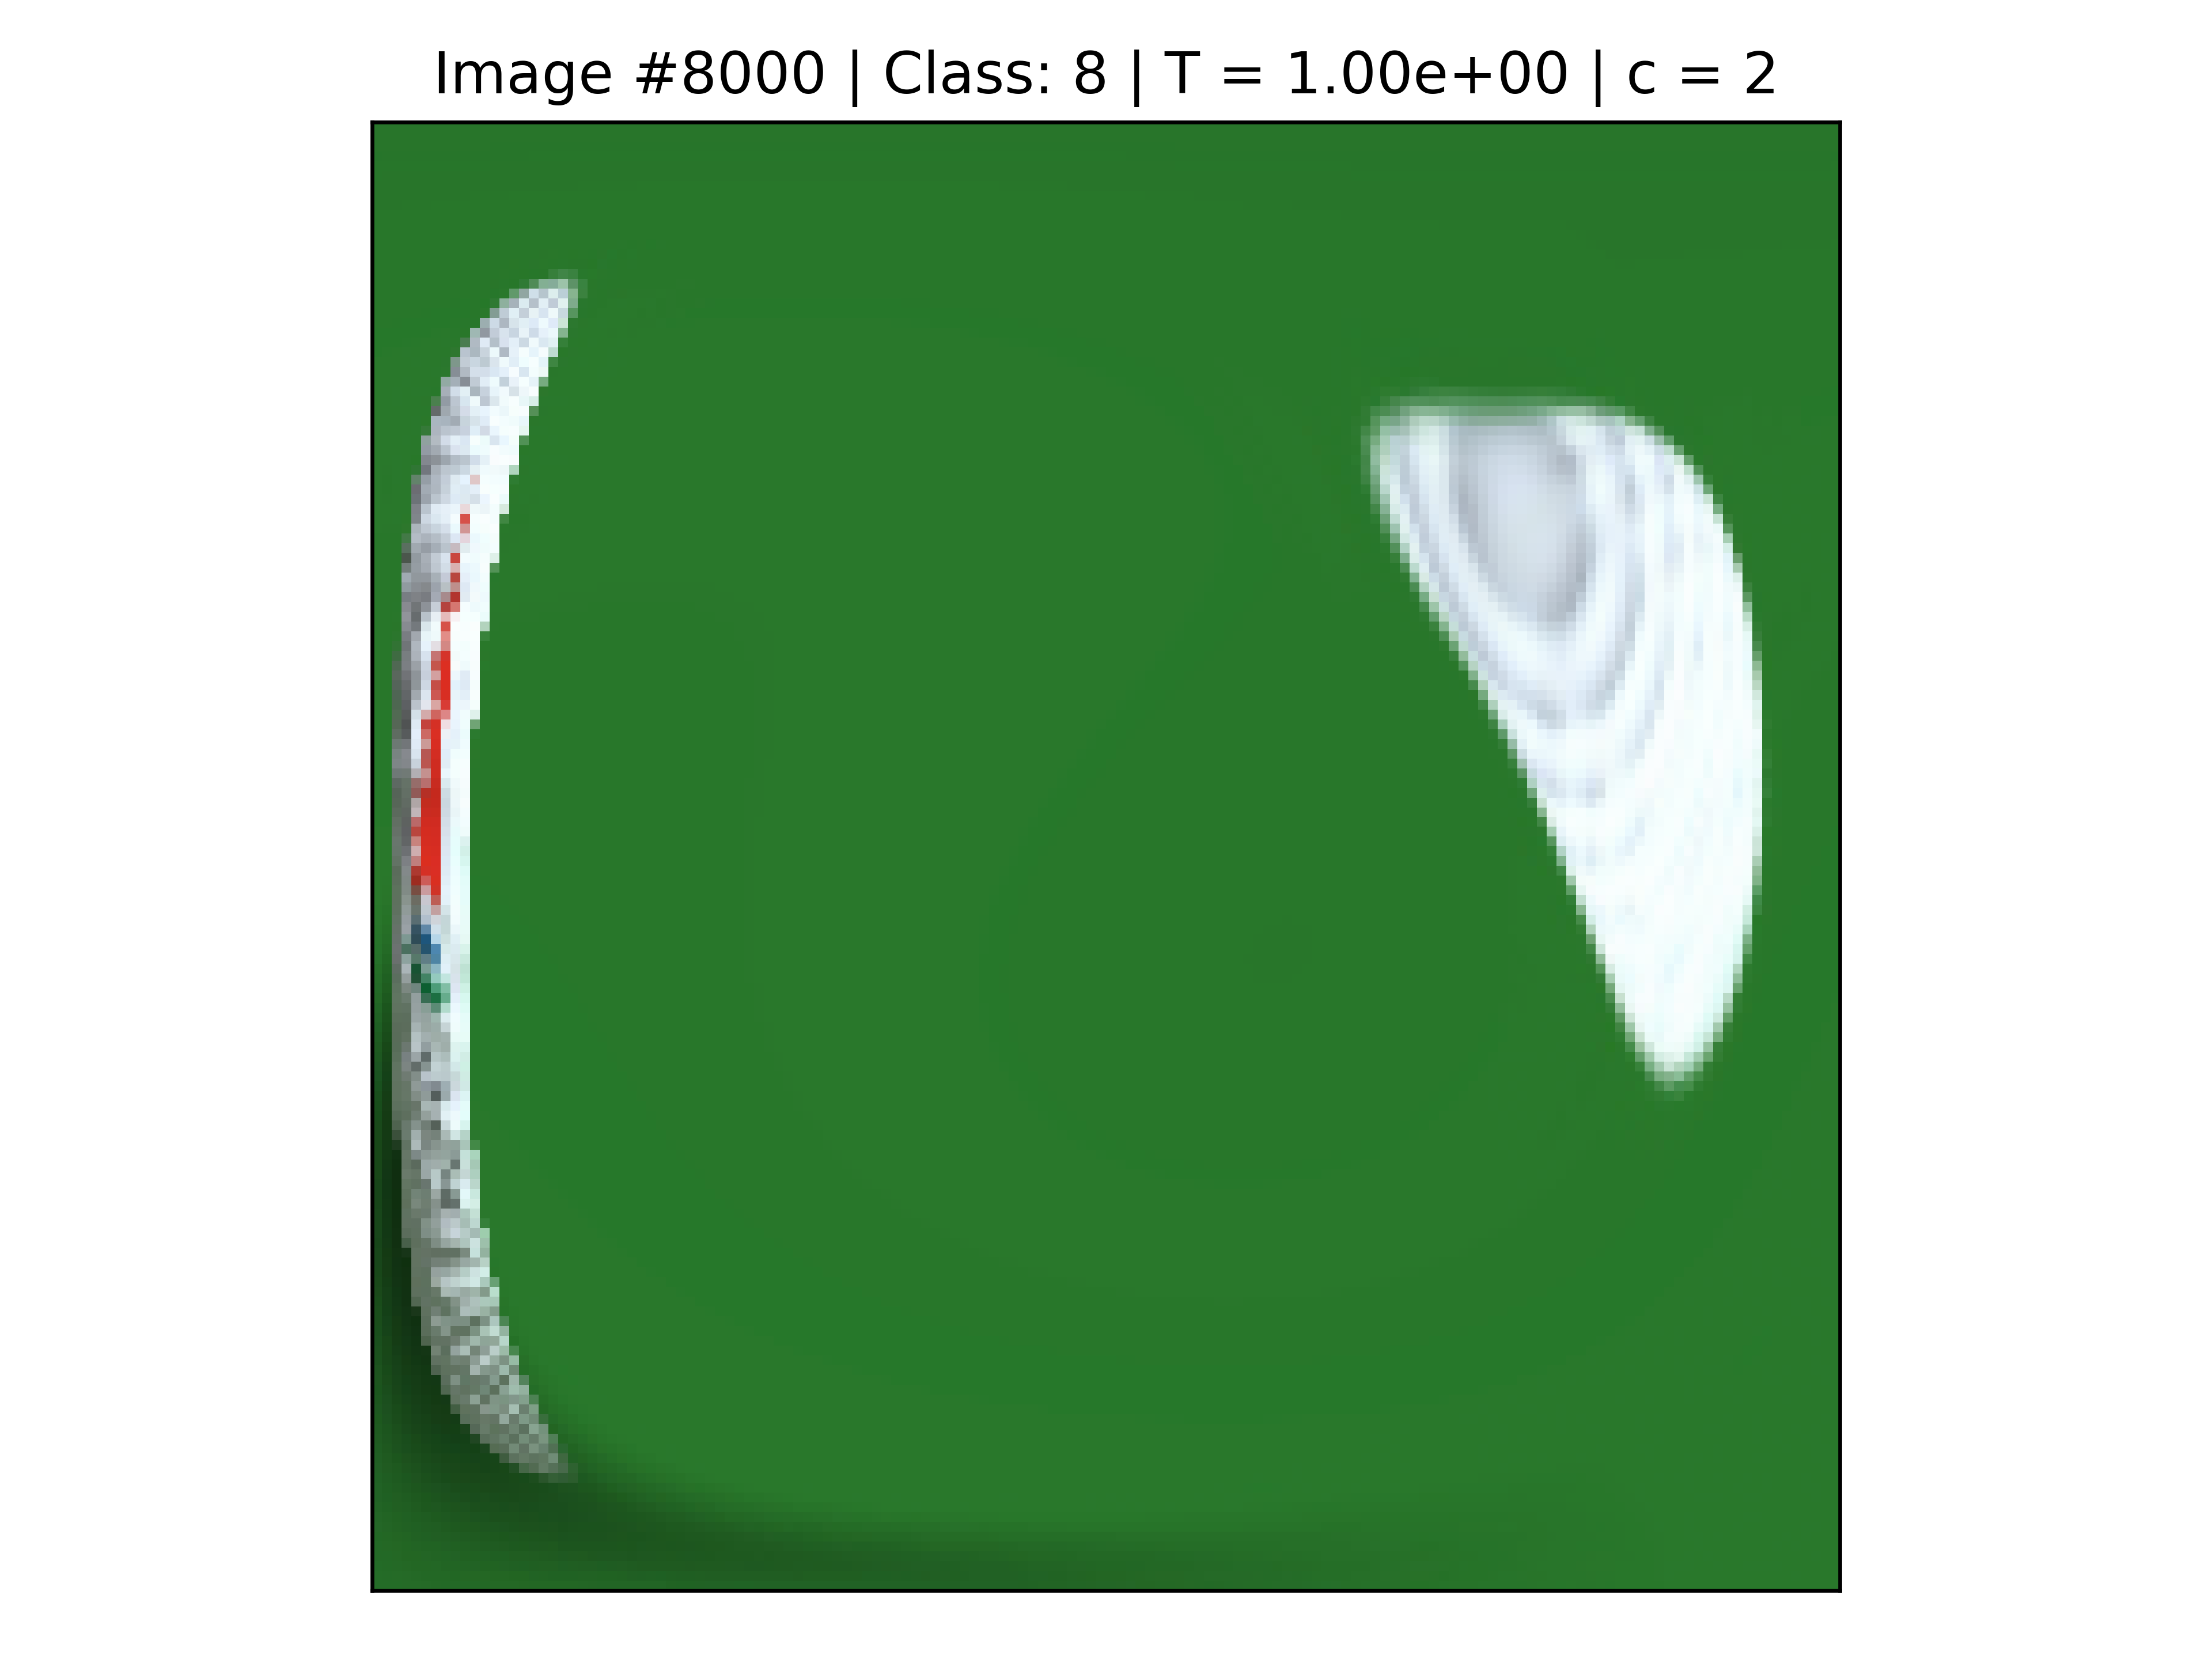
\includegraphics[width=\textwidth]{ch1-diffy/figures/warping_examples/8000_0_1.png}
%    \caption{$T=1$}
%    % \label{fig:my_label}
%    \end{subfigure}
%    \begin{subfigure}{0.18\textwidth}
%    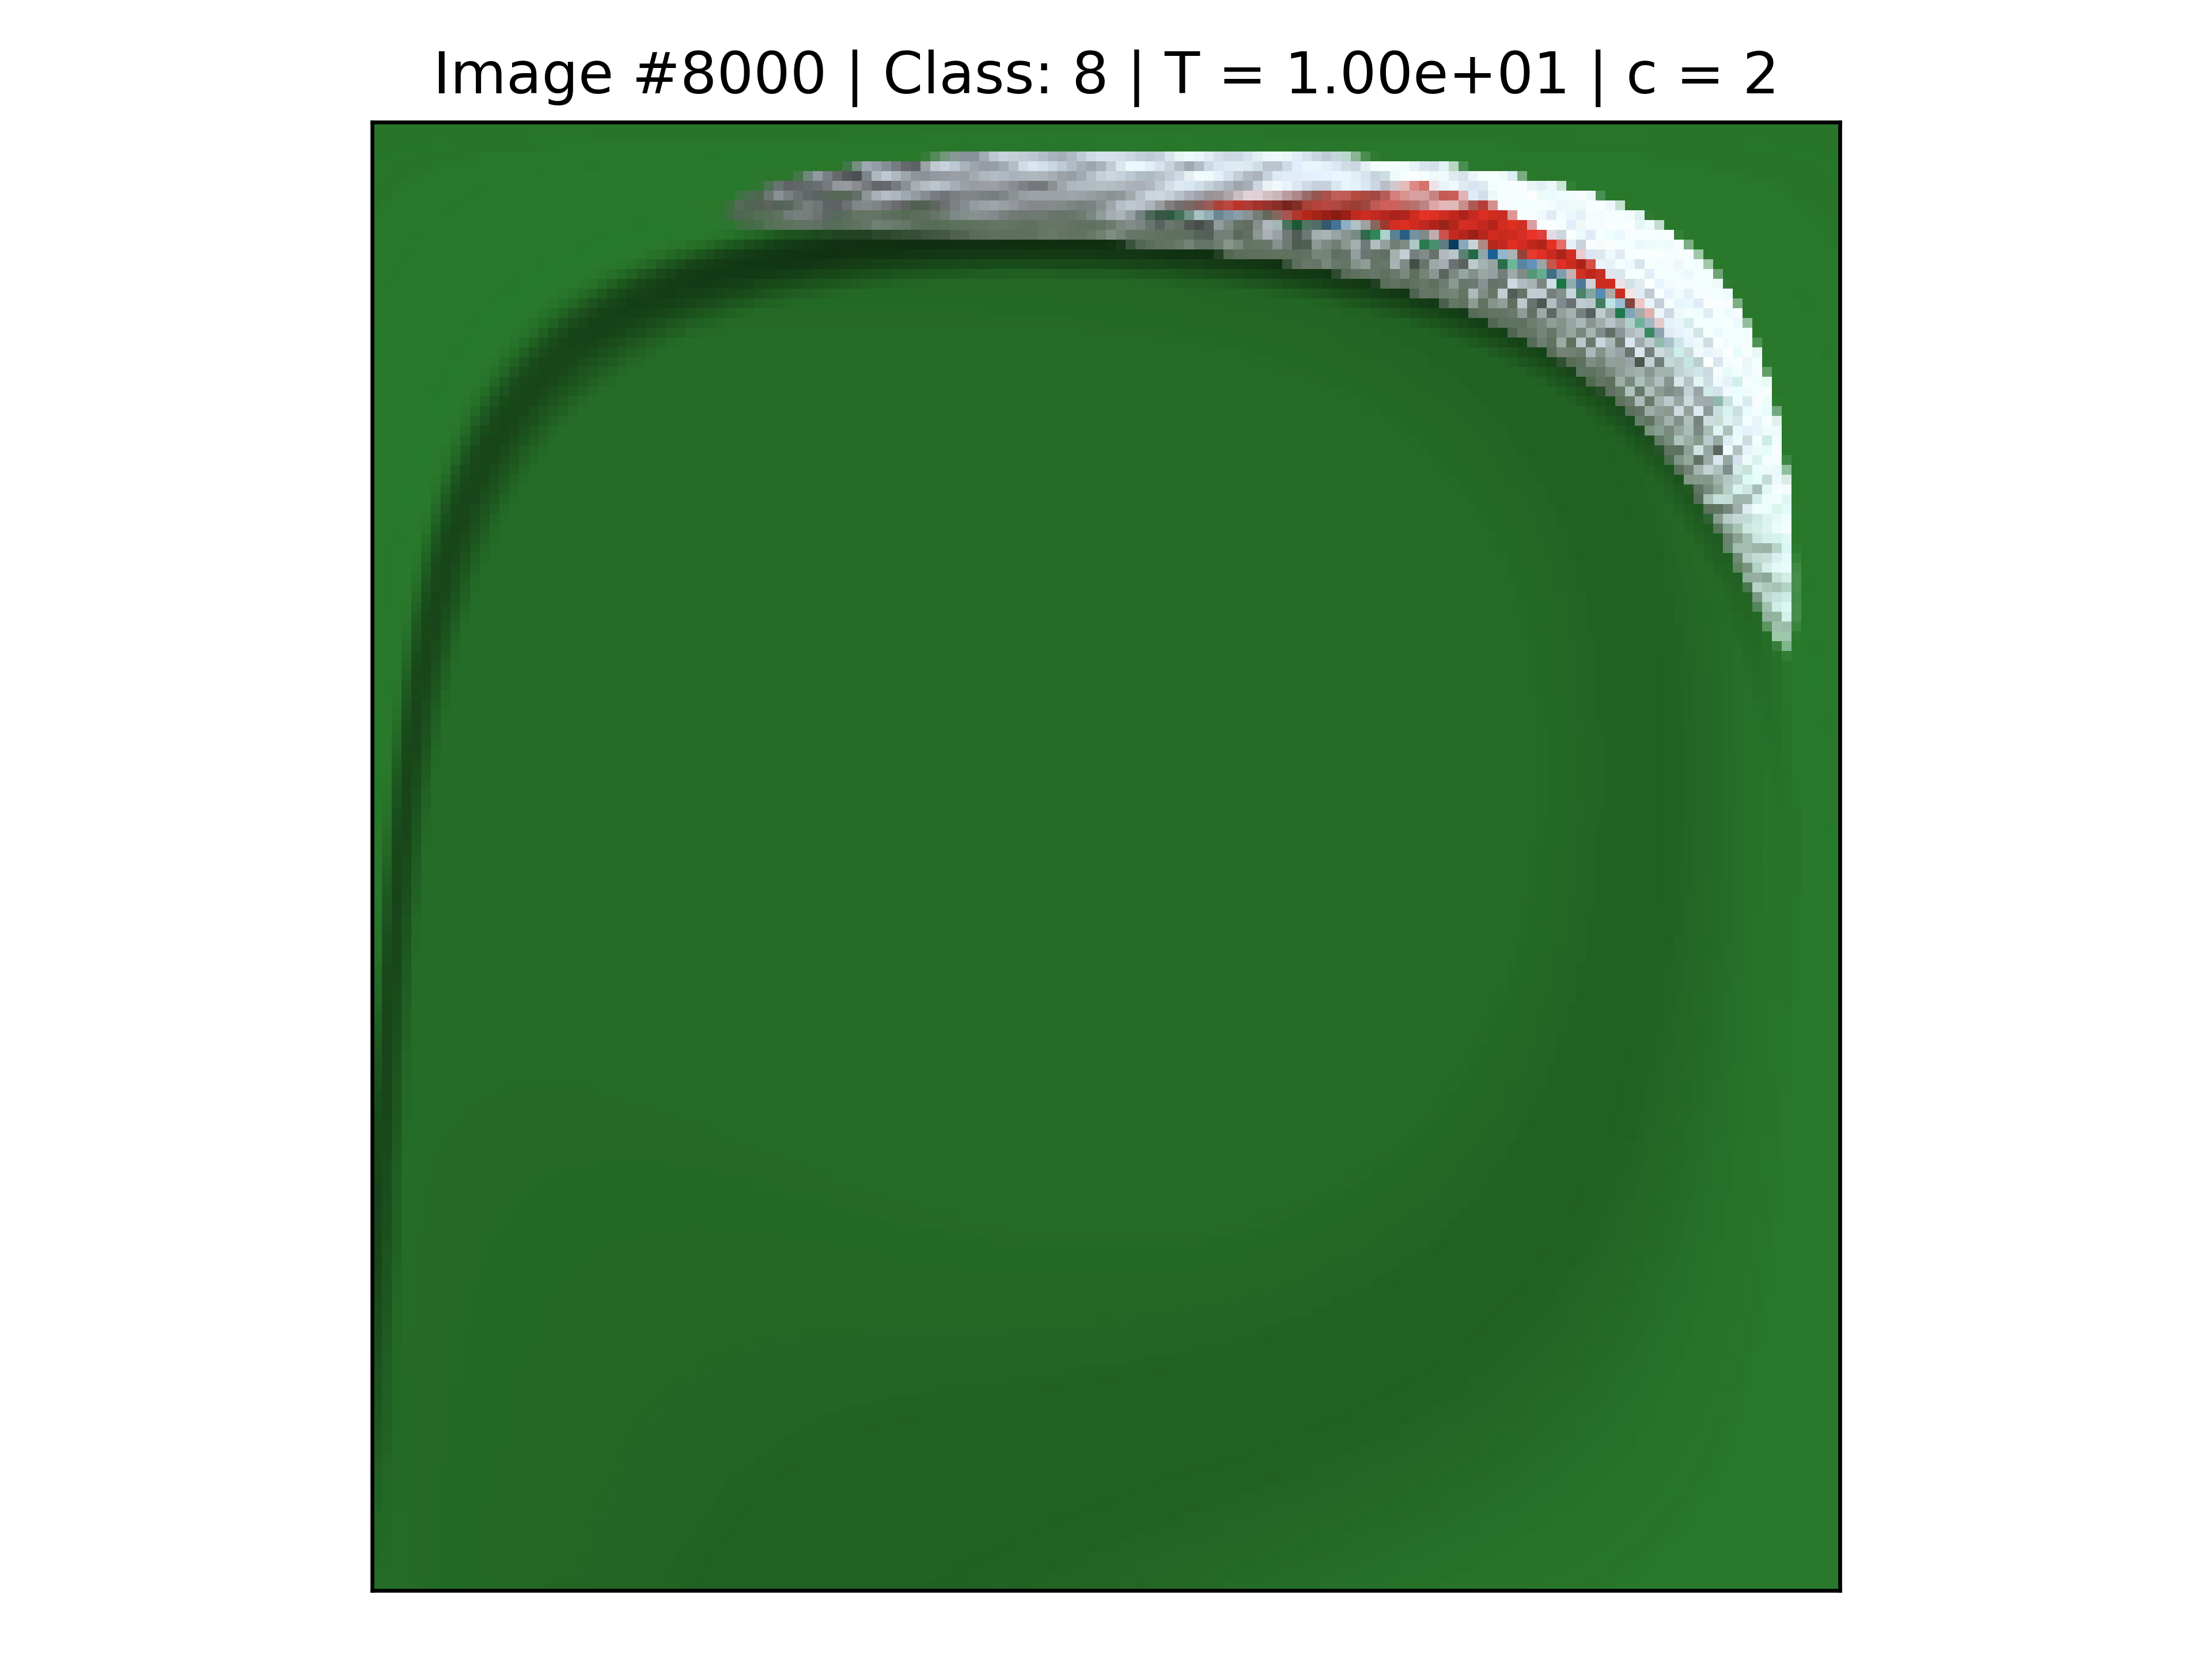
\includegraphics[width=\textwidth]{ch1-diffy/figures/warping_examples/8000_-1_1.png}
%    \caption{$T=10$}
%    % \label{fig:my_label}
%    \end{subfigure}
%    %%%%%
%    \begin{subfigure}{0.18\textwidth}
%    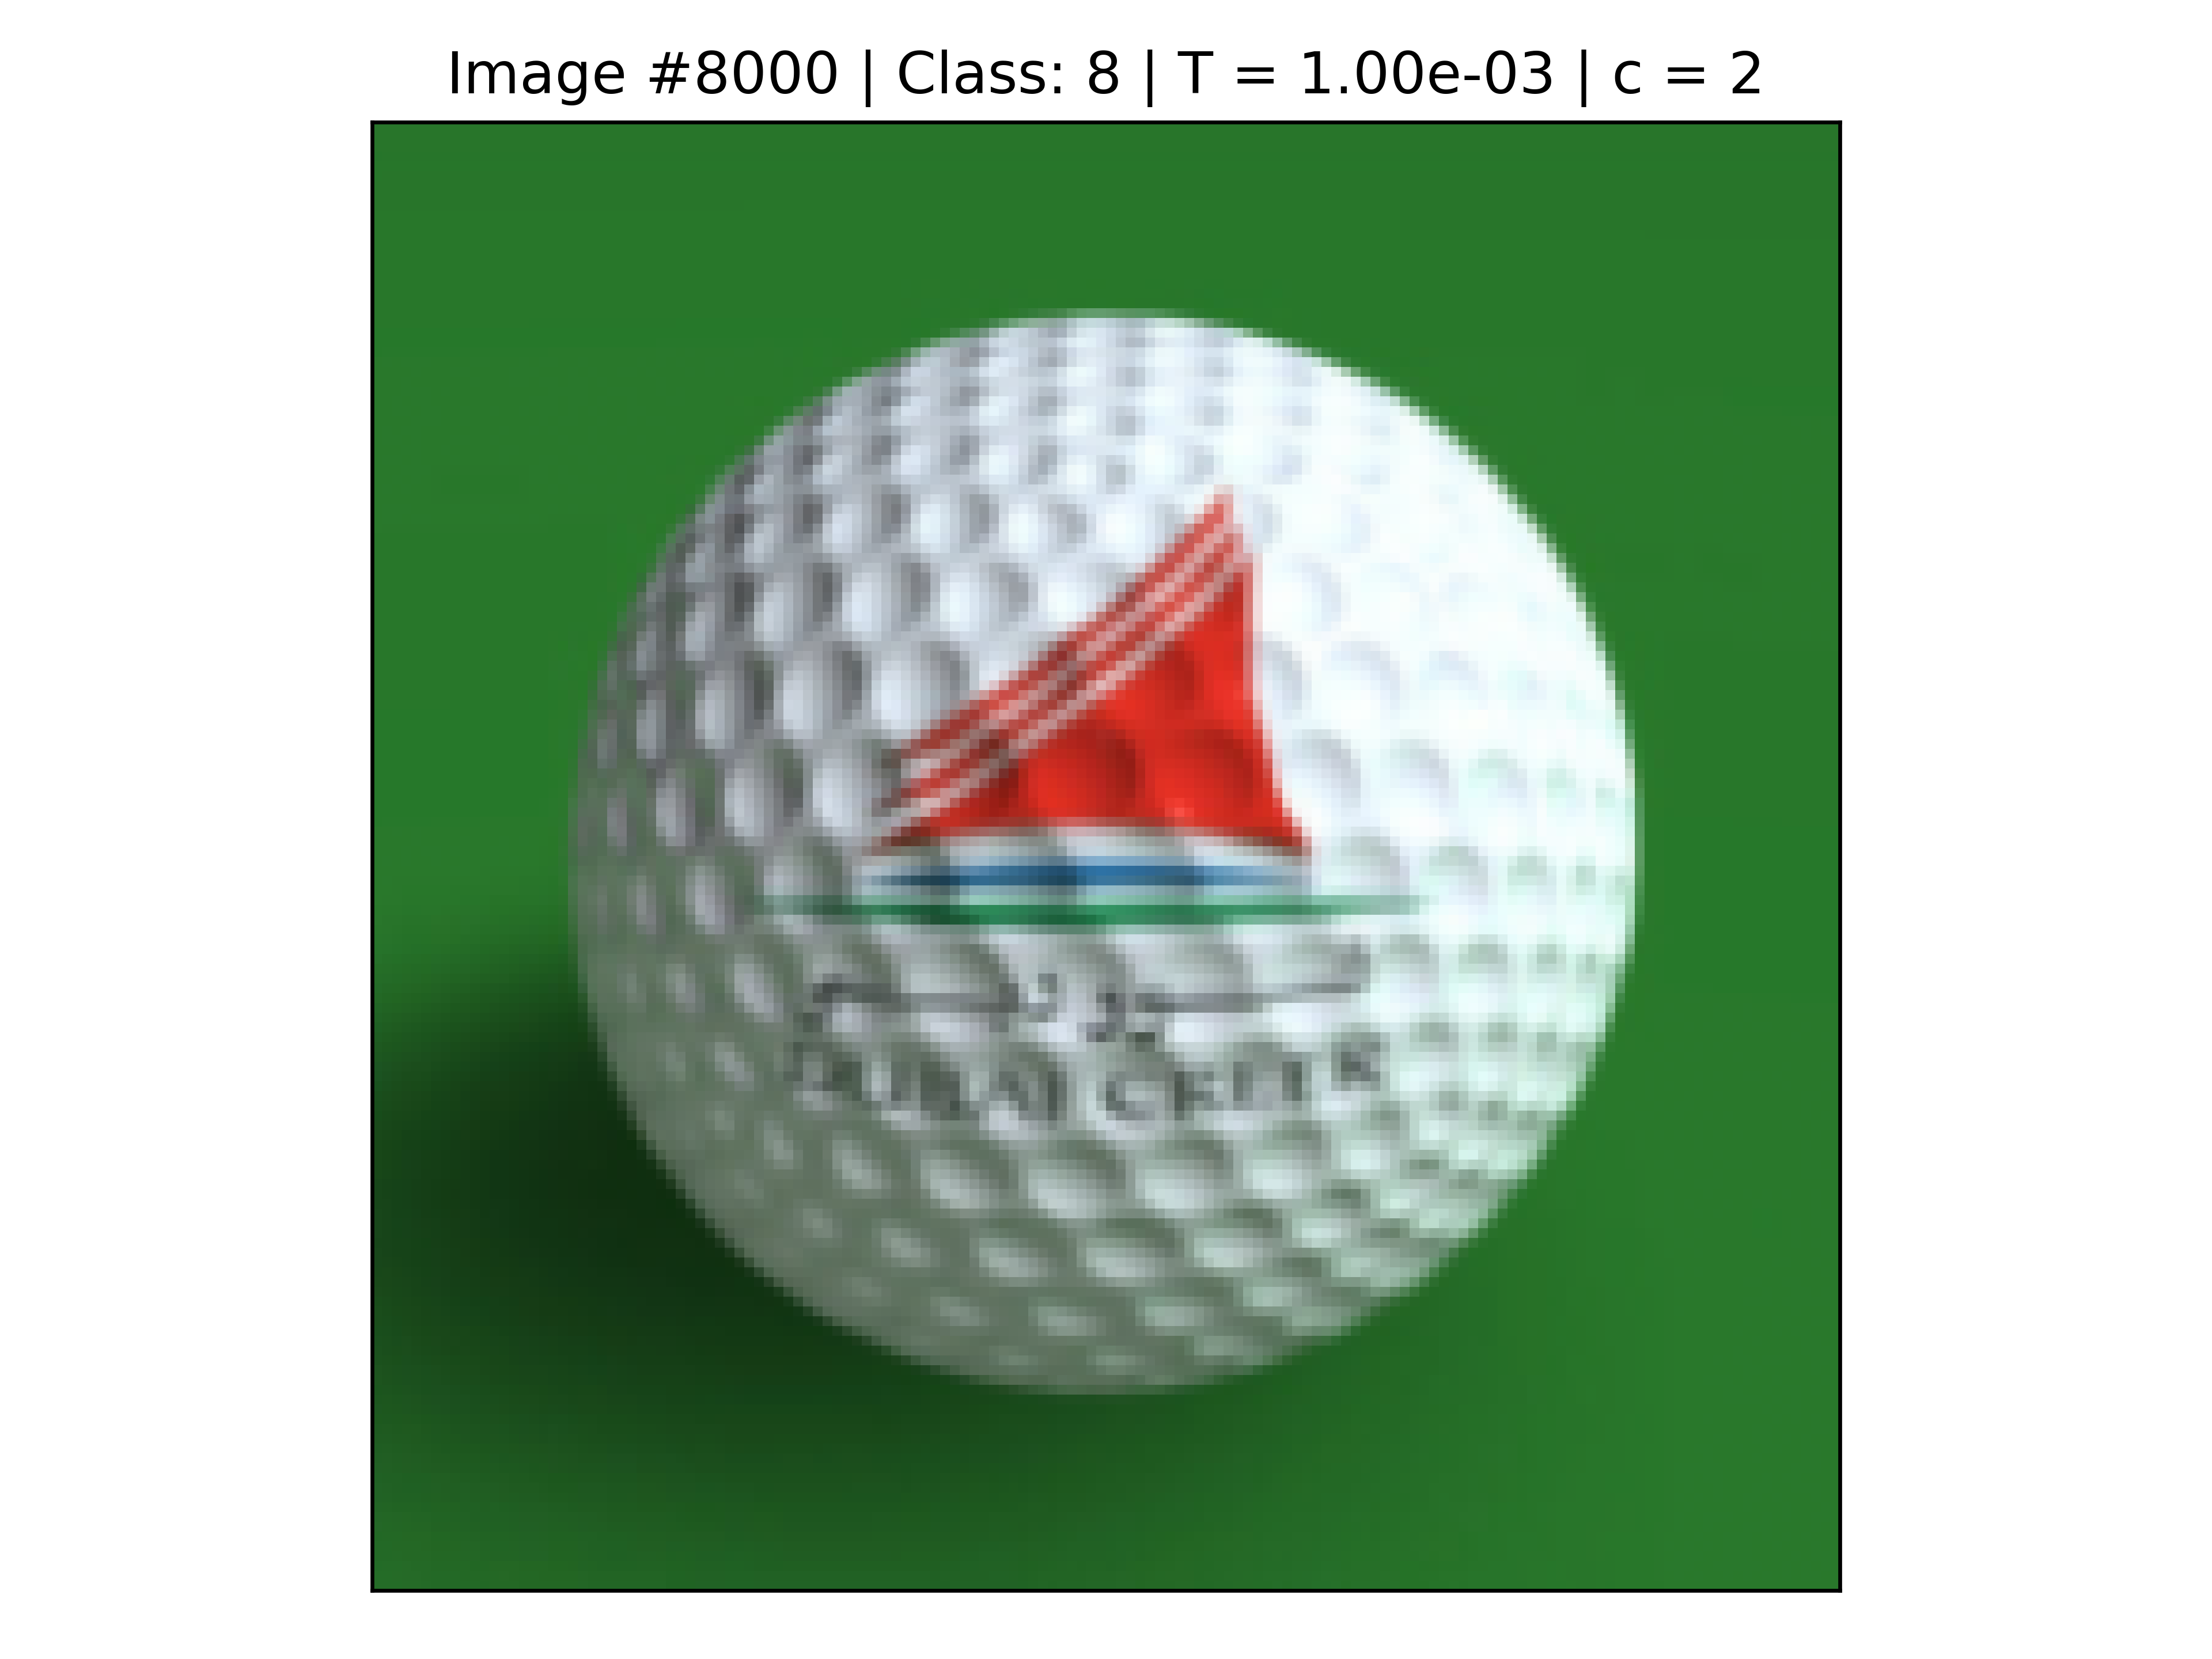
\includegraphics[width=\textwidth]{ch1-diffy/figures/warping_examples/8000_3_2.png}
%    \caption{$T=10^{-3}$}
%    % \label{fig:my_label}
%    \end{subfigure}
%    \begin{subfigure}{0.18\textwidth}
%    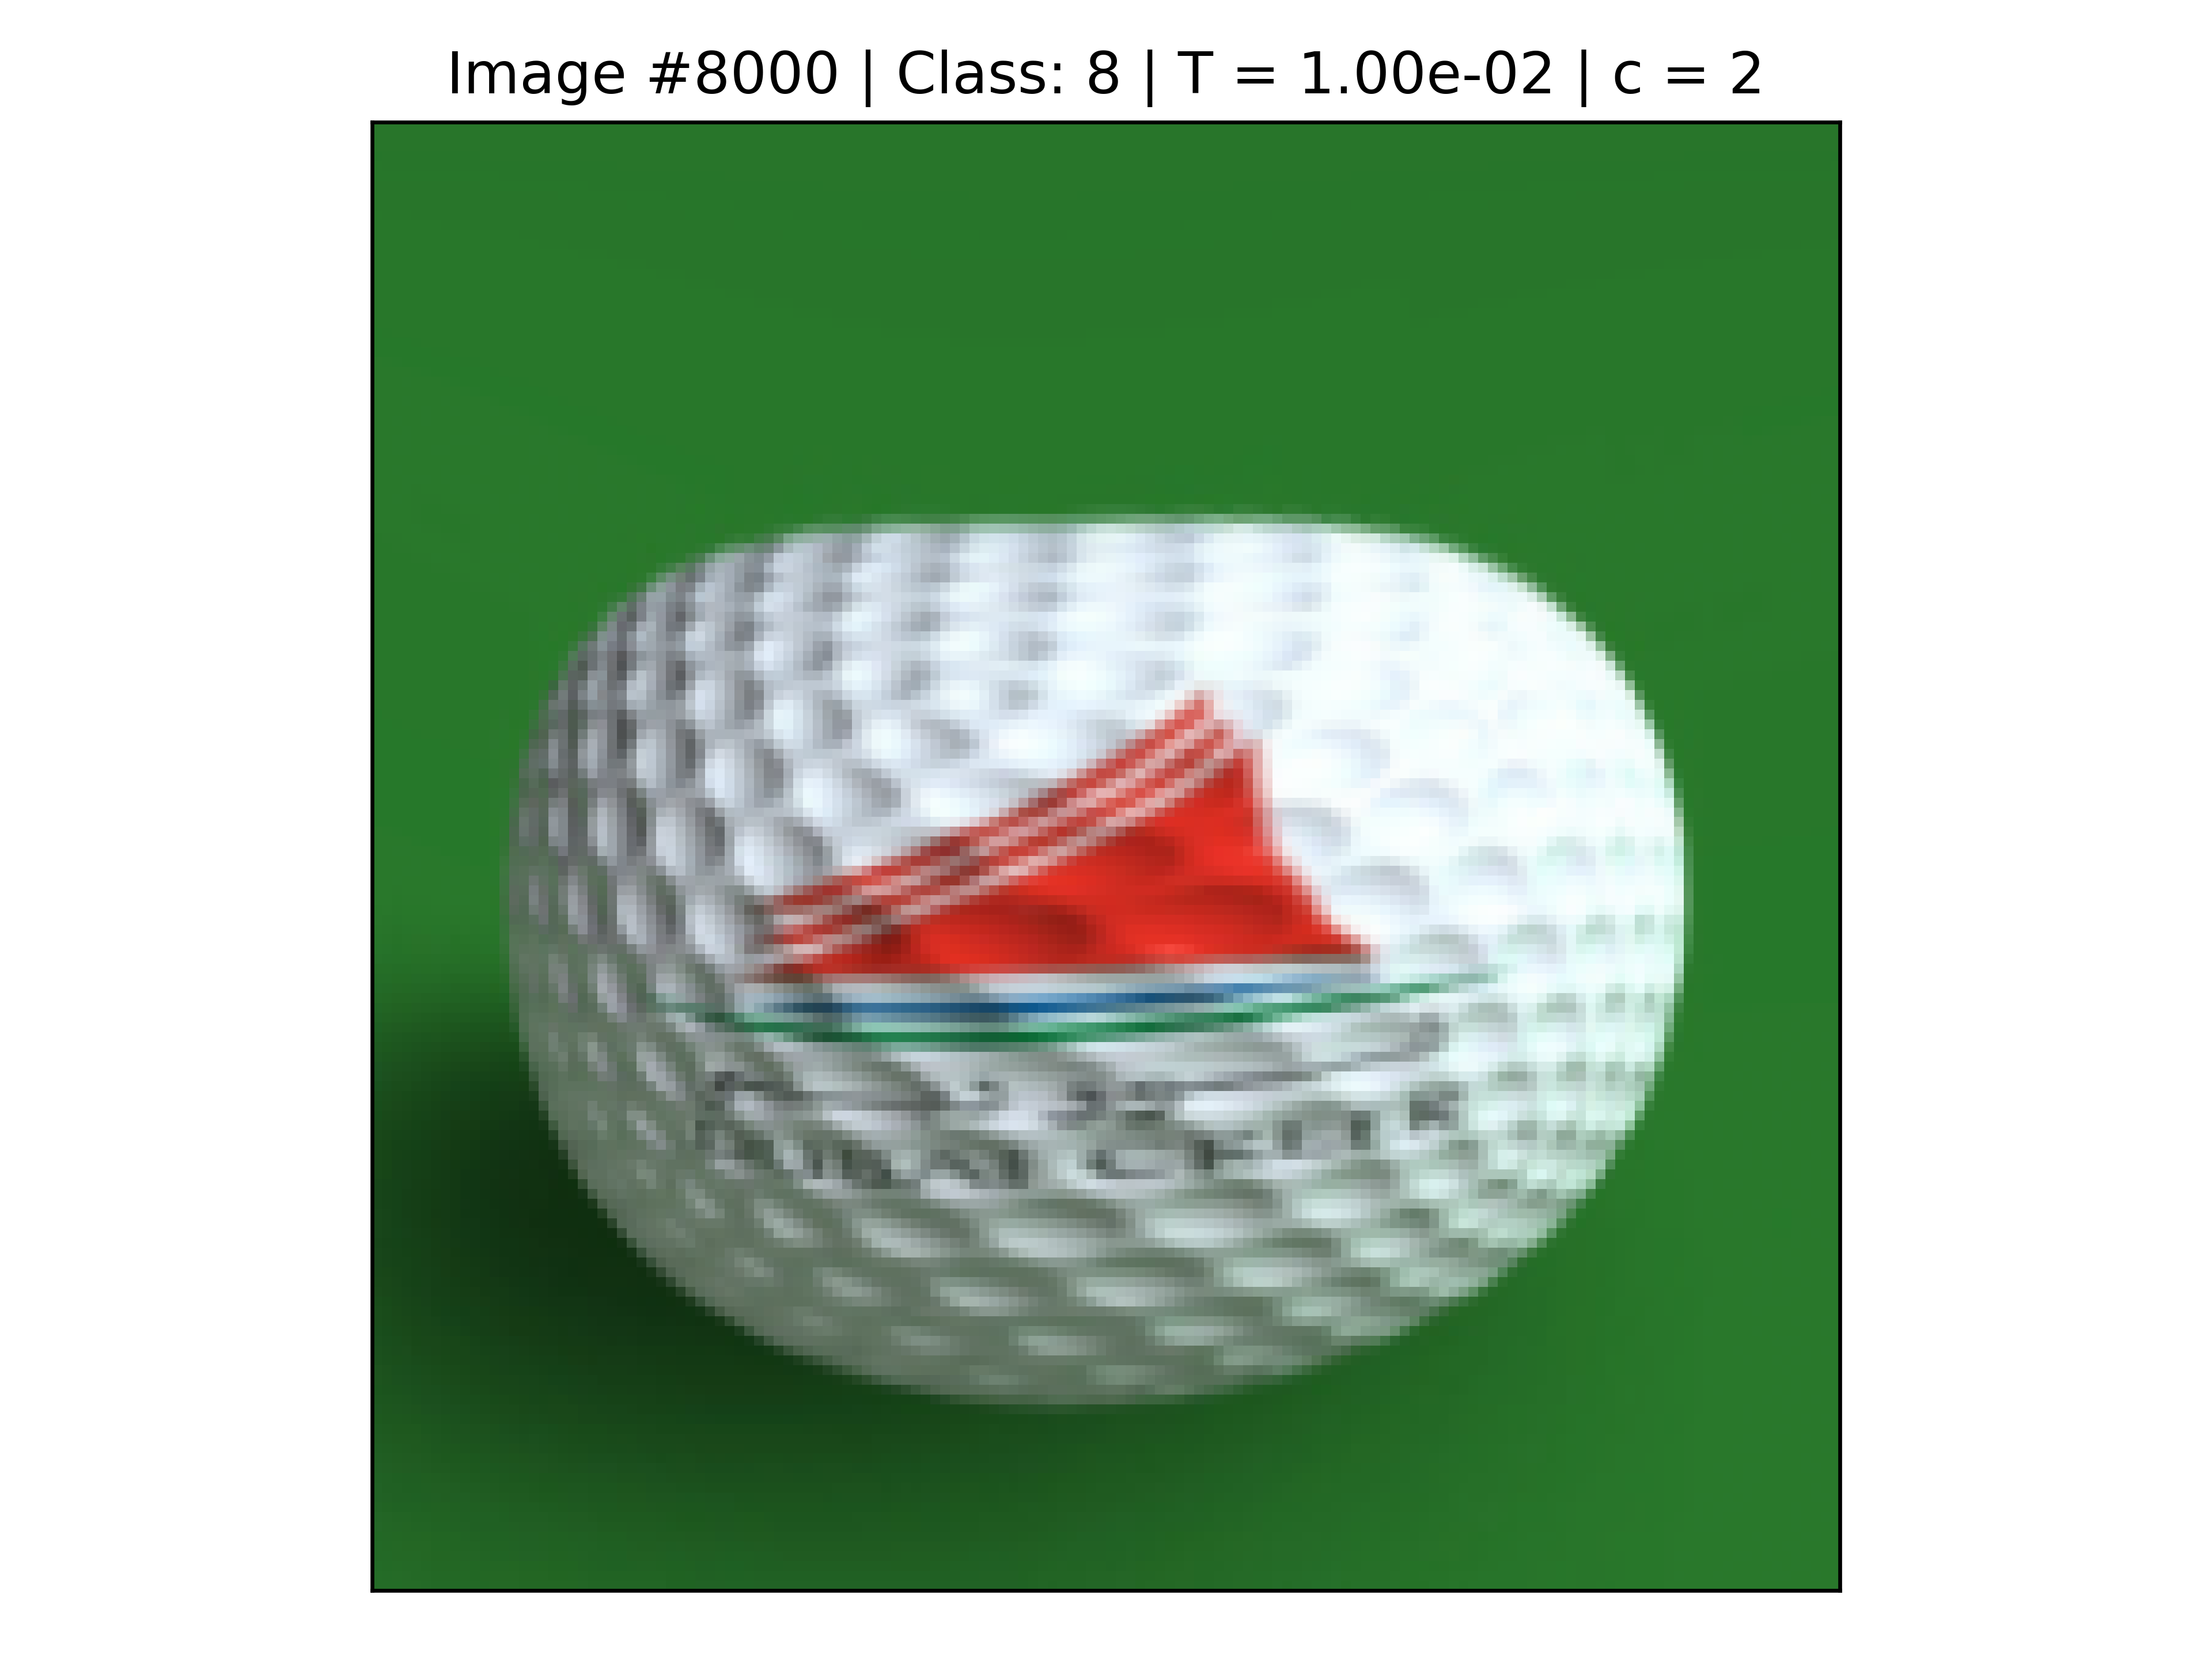
\includegraphics[width=\textwidth]{ch1-diffy/figures/warping_examples/8000_2_2.png}
%    \caption{$T=10^{-2}$}
%    % \label{fig:my_label}
%    \end{subfigure}
%    \begin{subfigure}{0.18\textwidth}
%    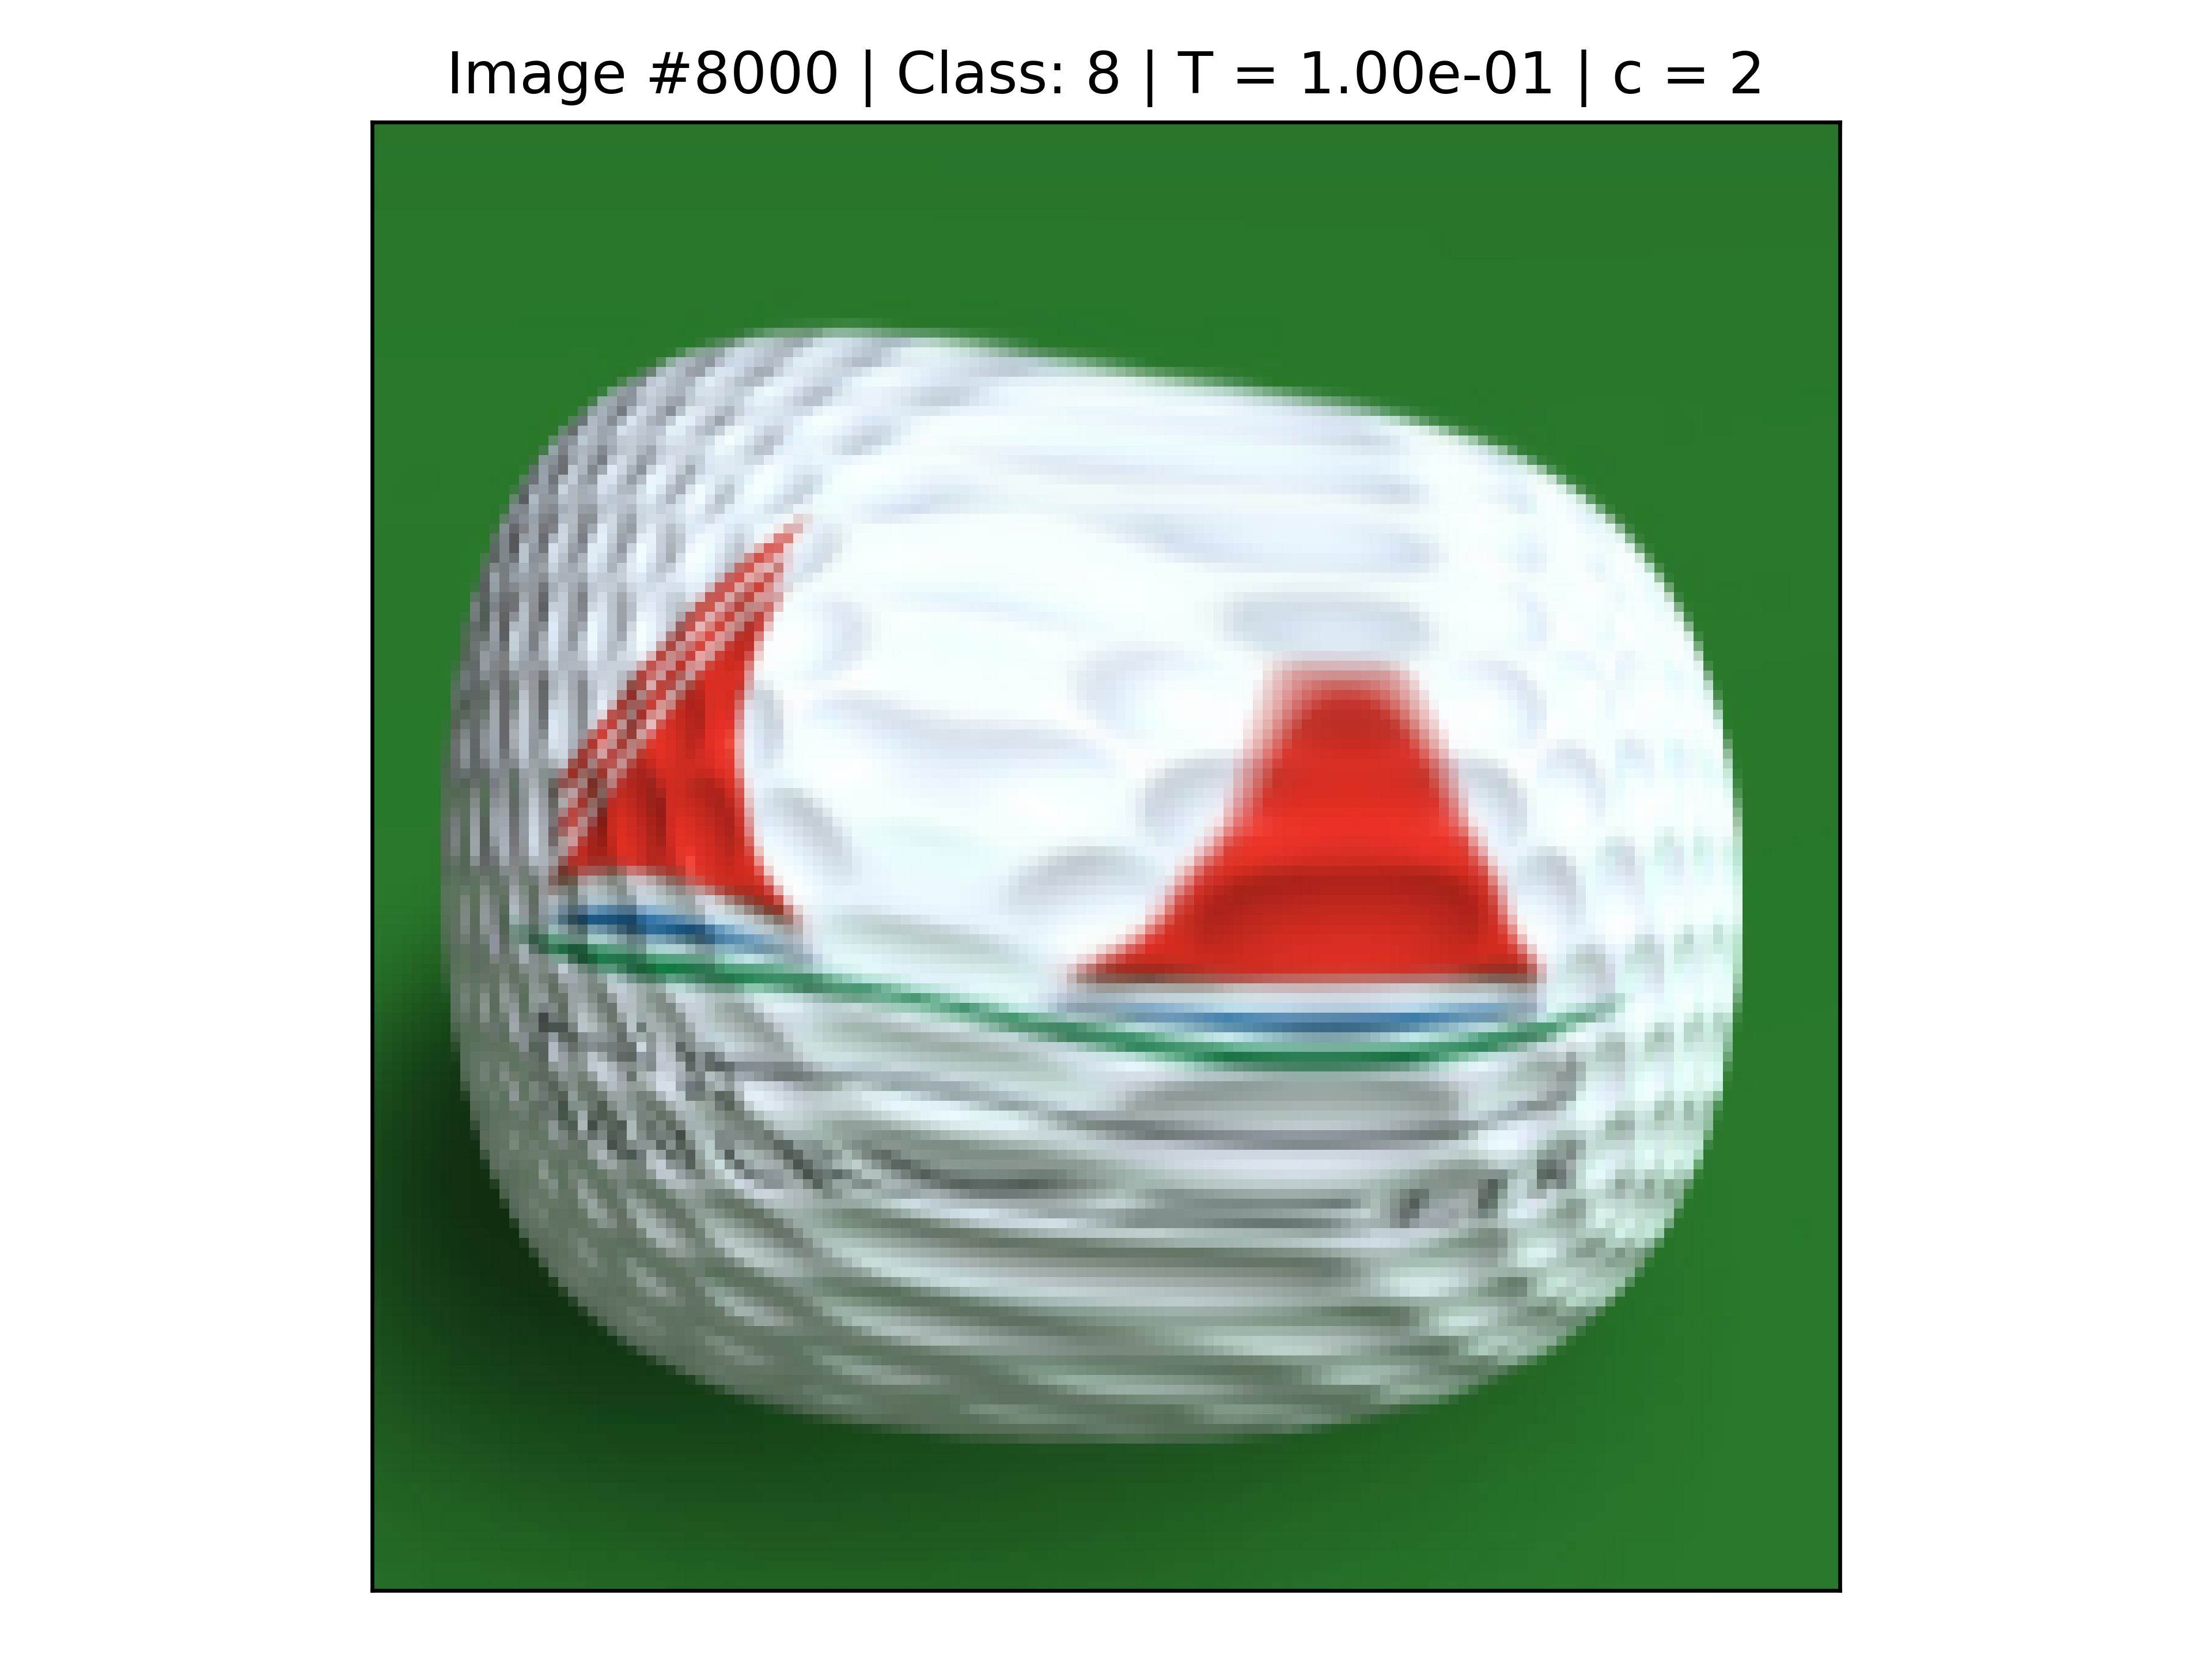
\includegraphics[width=\textwidth]{ch1-diffy/figures/warping_examples/8000_1_2.png}
%    \caption{$T=10^{-1}$}
%    % \label{fig:my_label}
%    \end{subfigure}
%    \begin{subfigure}{0.18\textwidth}
%    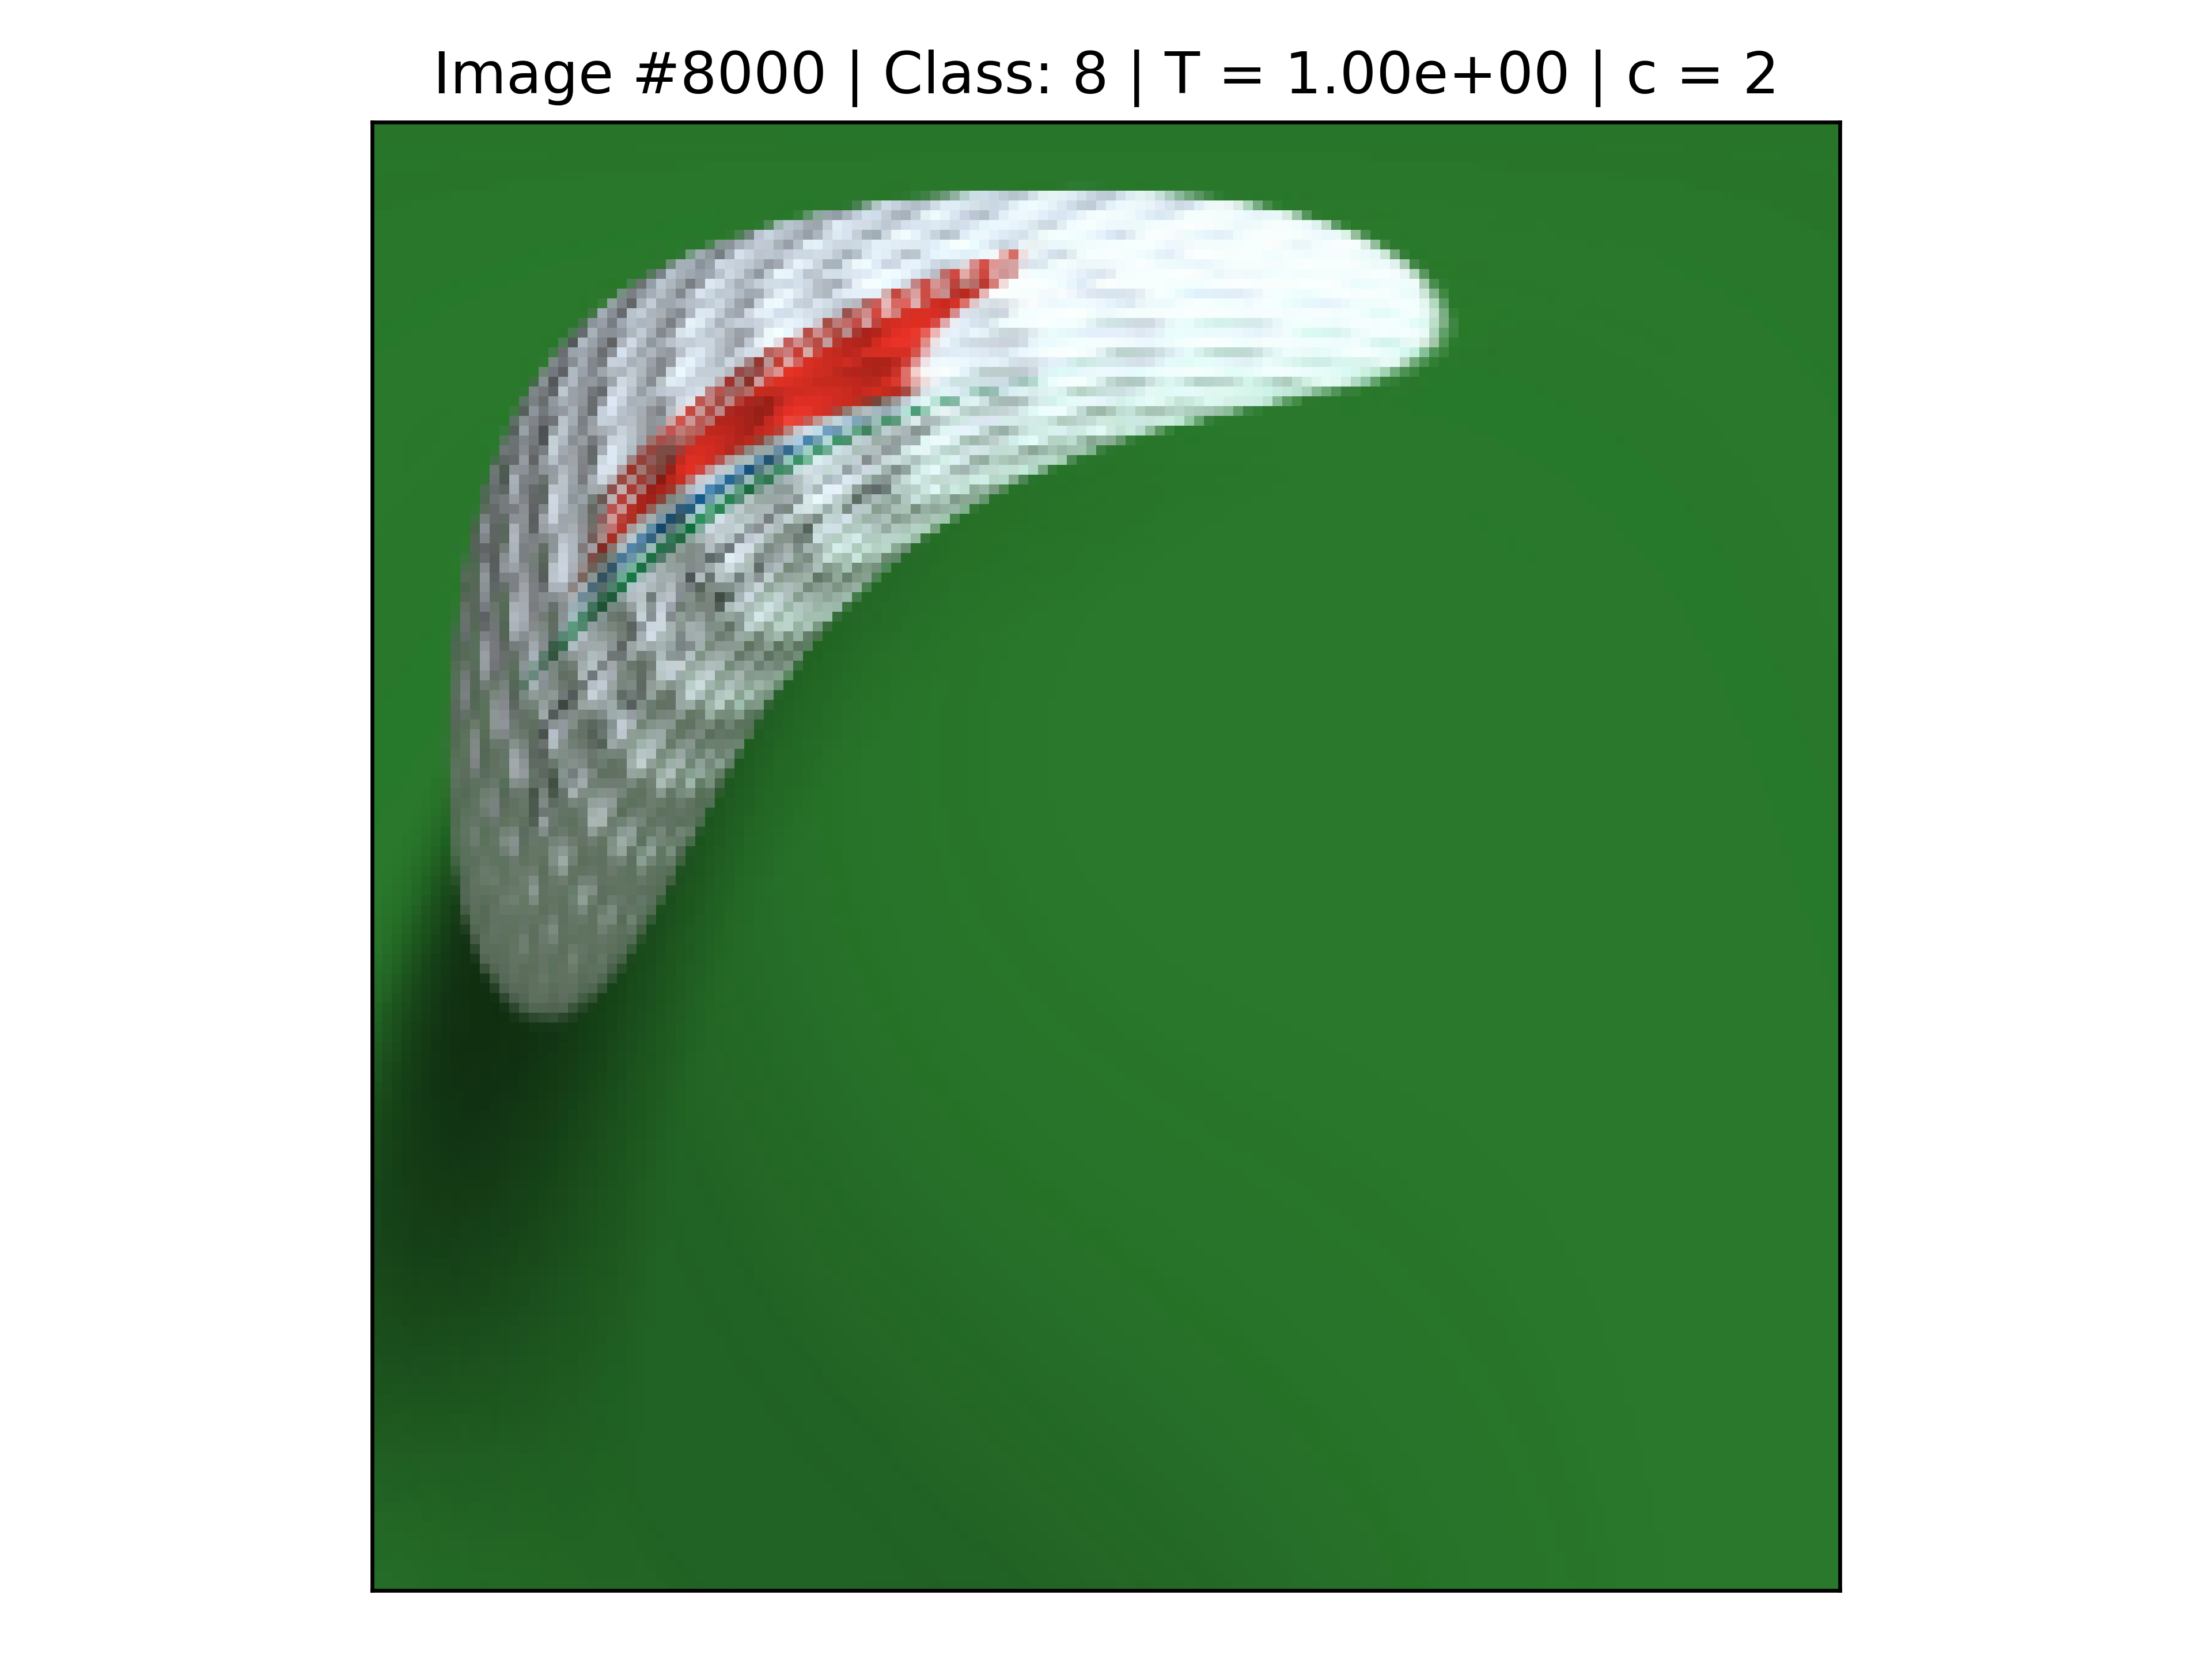
\includegraphics[width=\textwidth]{ch1-diffy/figures/warping_examples/8000_0_2.png}
%    \caption{$T=1$}
%    % \label{fig:my_label}
%    \end{subfigure}
%    \begin{subfigure}{0.18\textwidth}
%    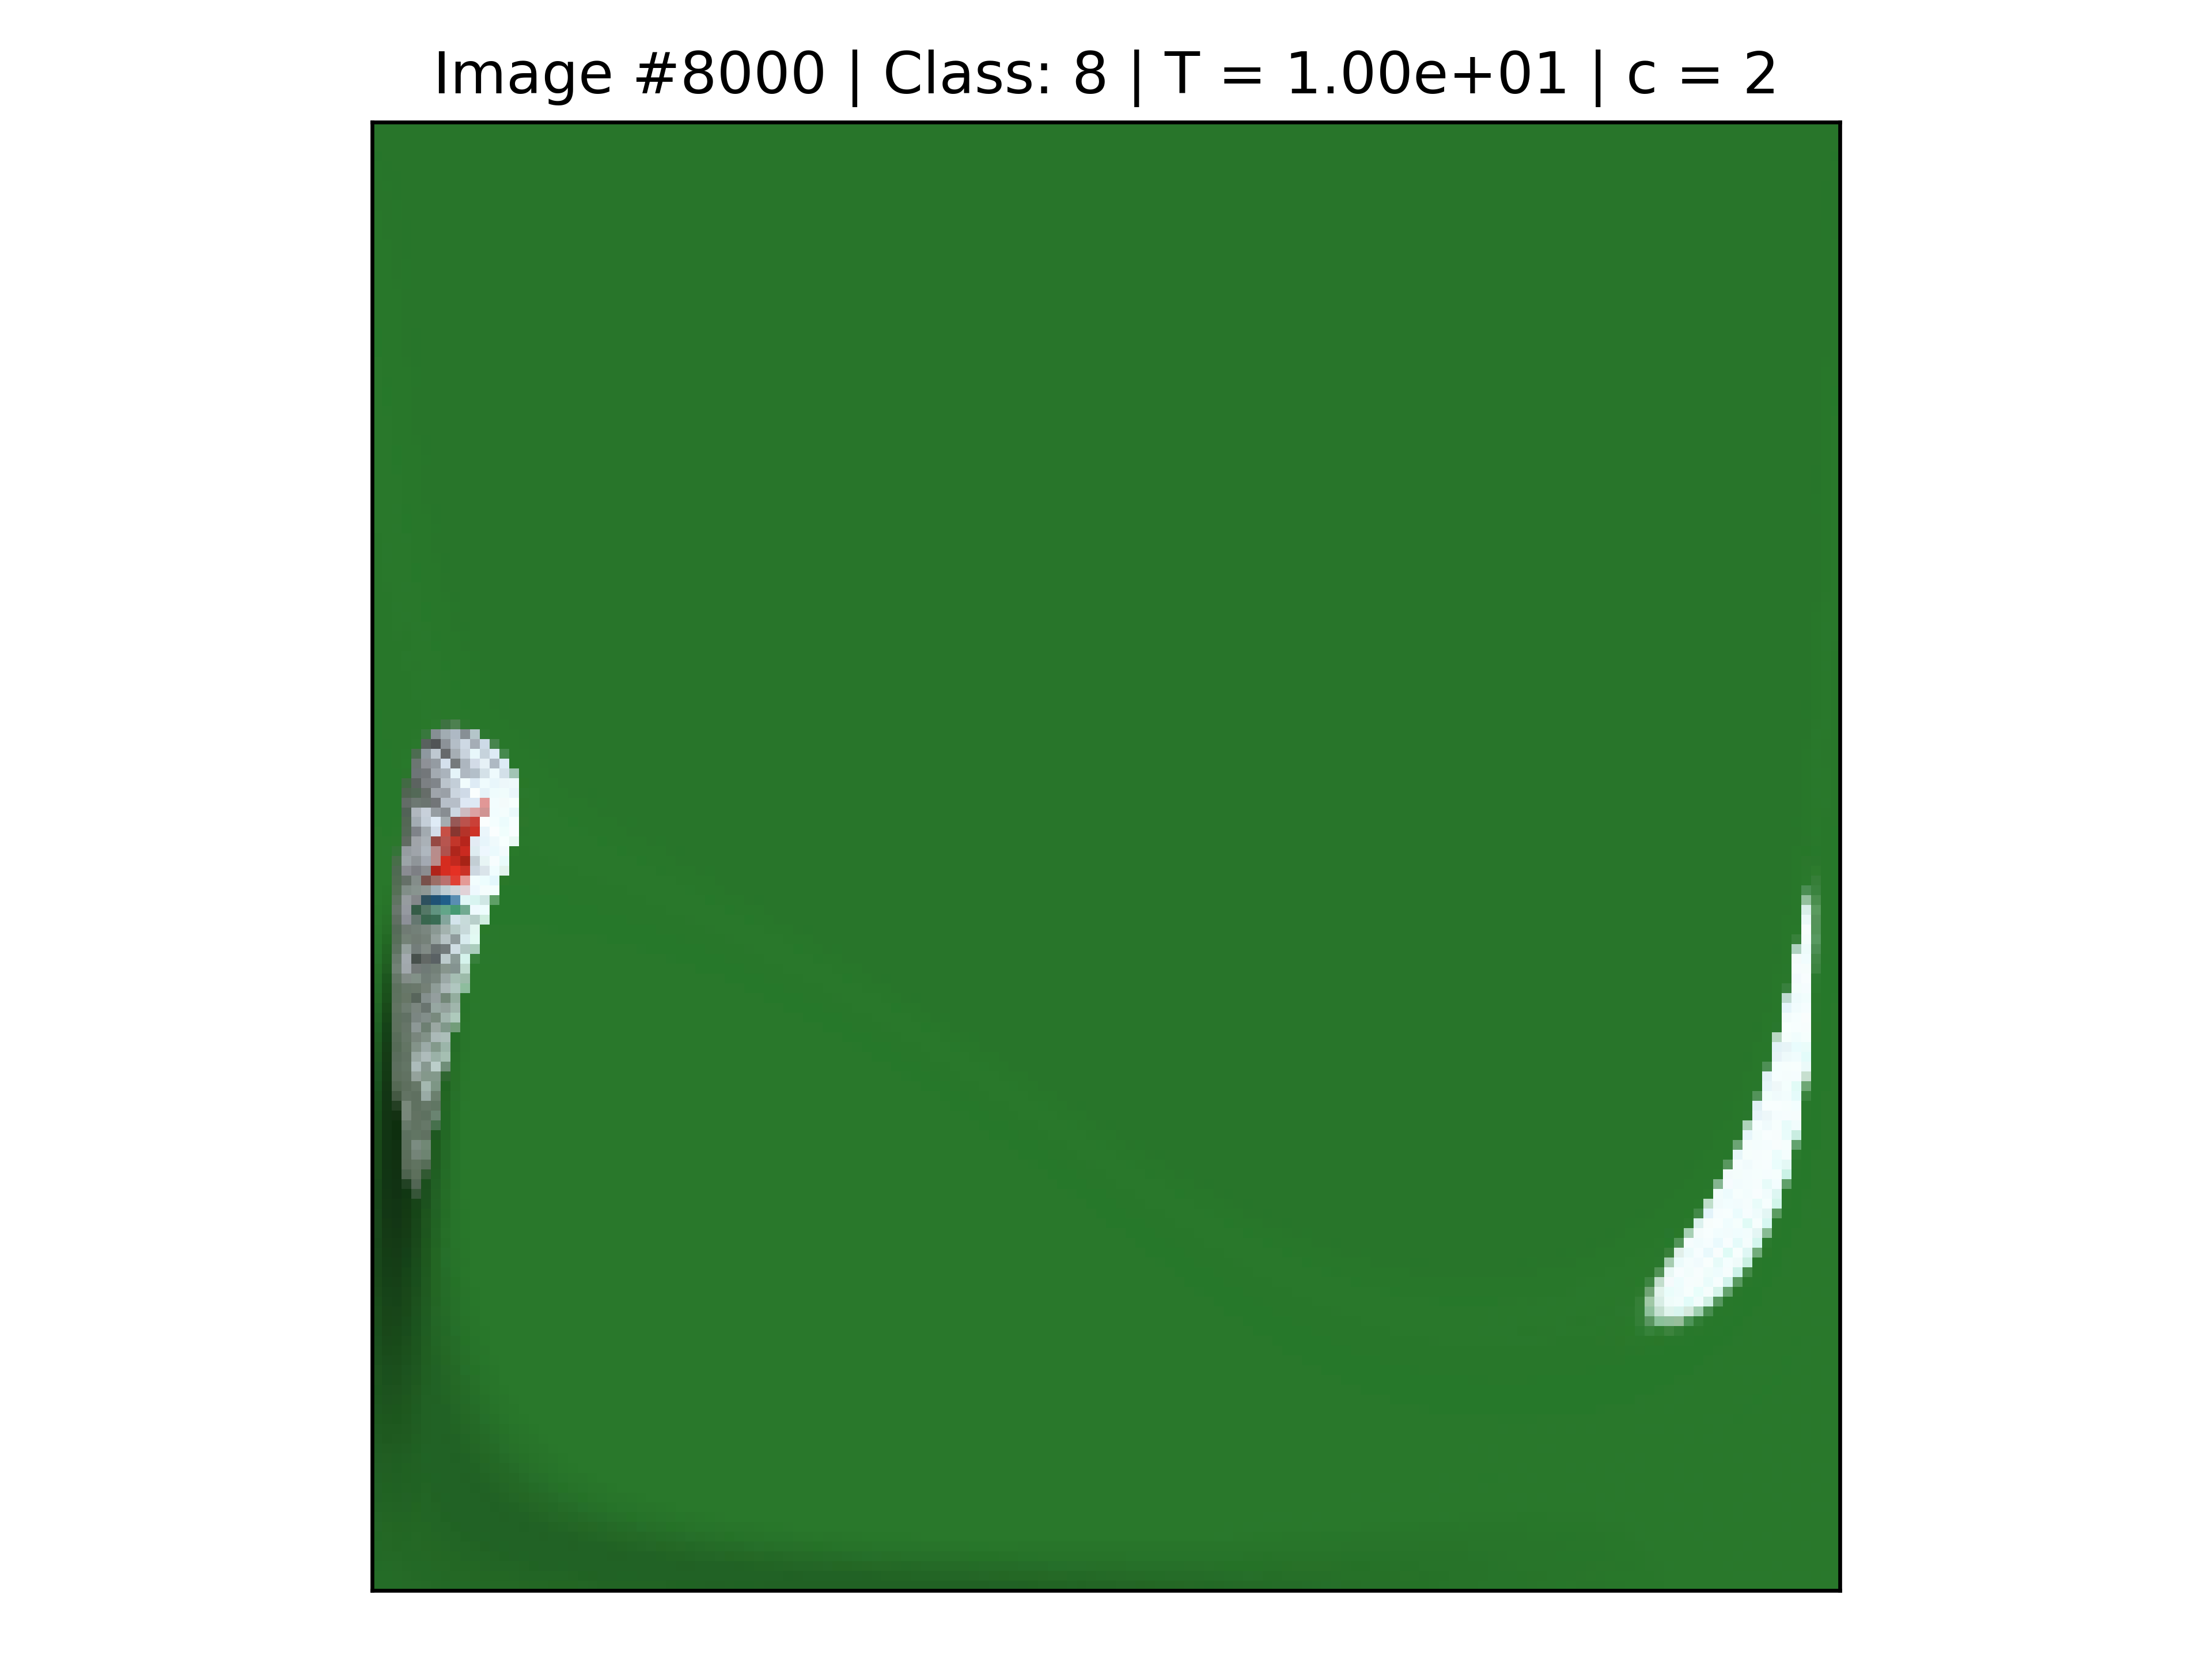
\includegraphics[width=\textwidth]{ch1-diffy/figures/warping_examples/8000_-1_2.png}
%    \caption{$T=10$}
%    % \label{fig:my_label}
%    \end{subfigure}
%    %%%%%
%    \centering
%    \begin{subfigure}{0.18\textwidth}
%    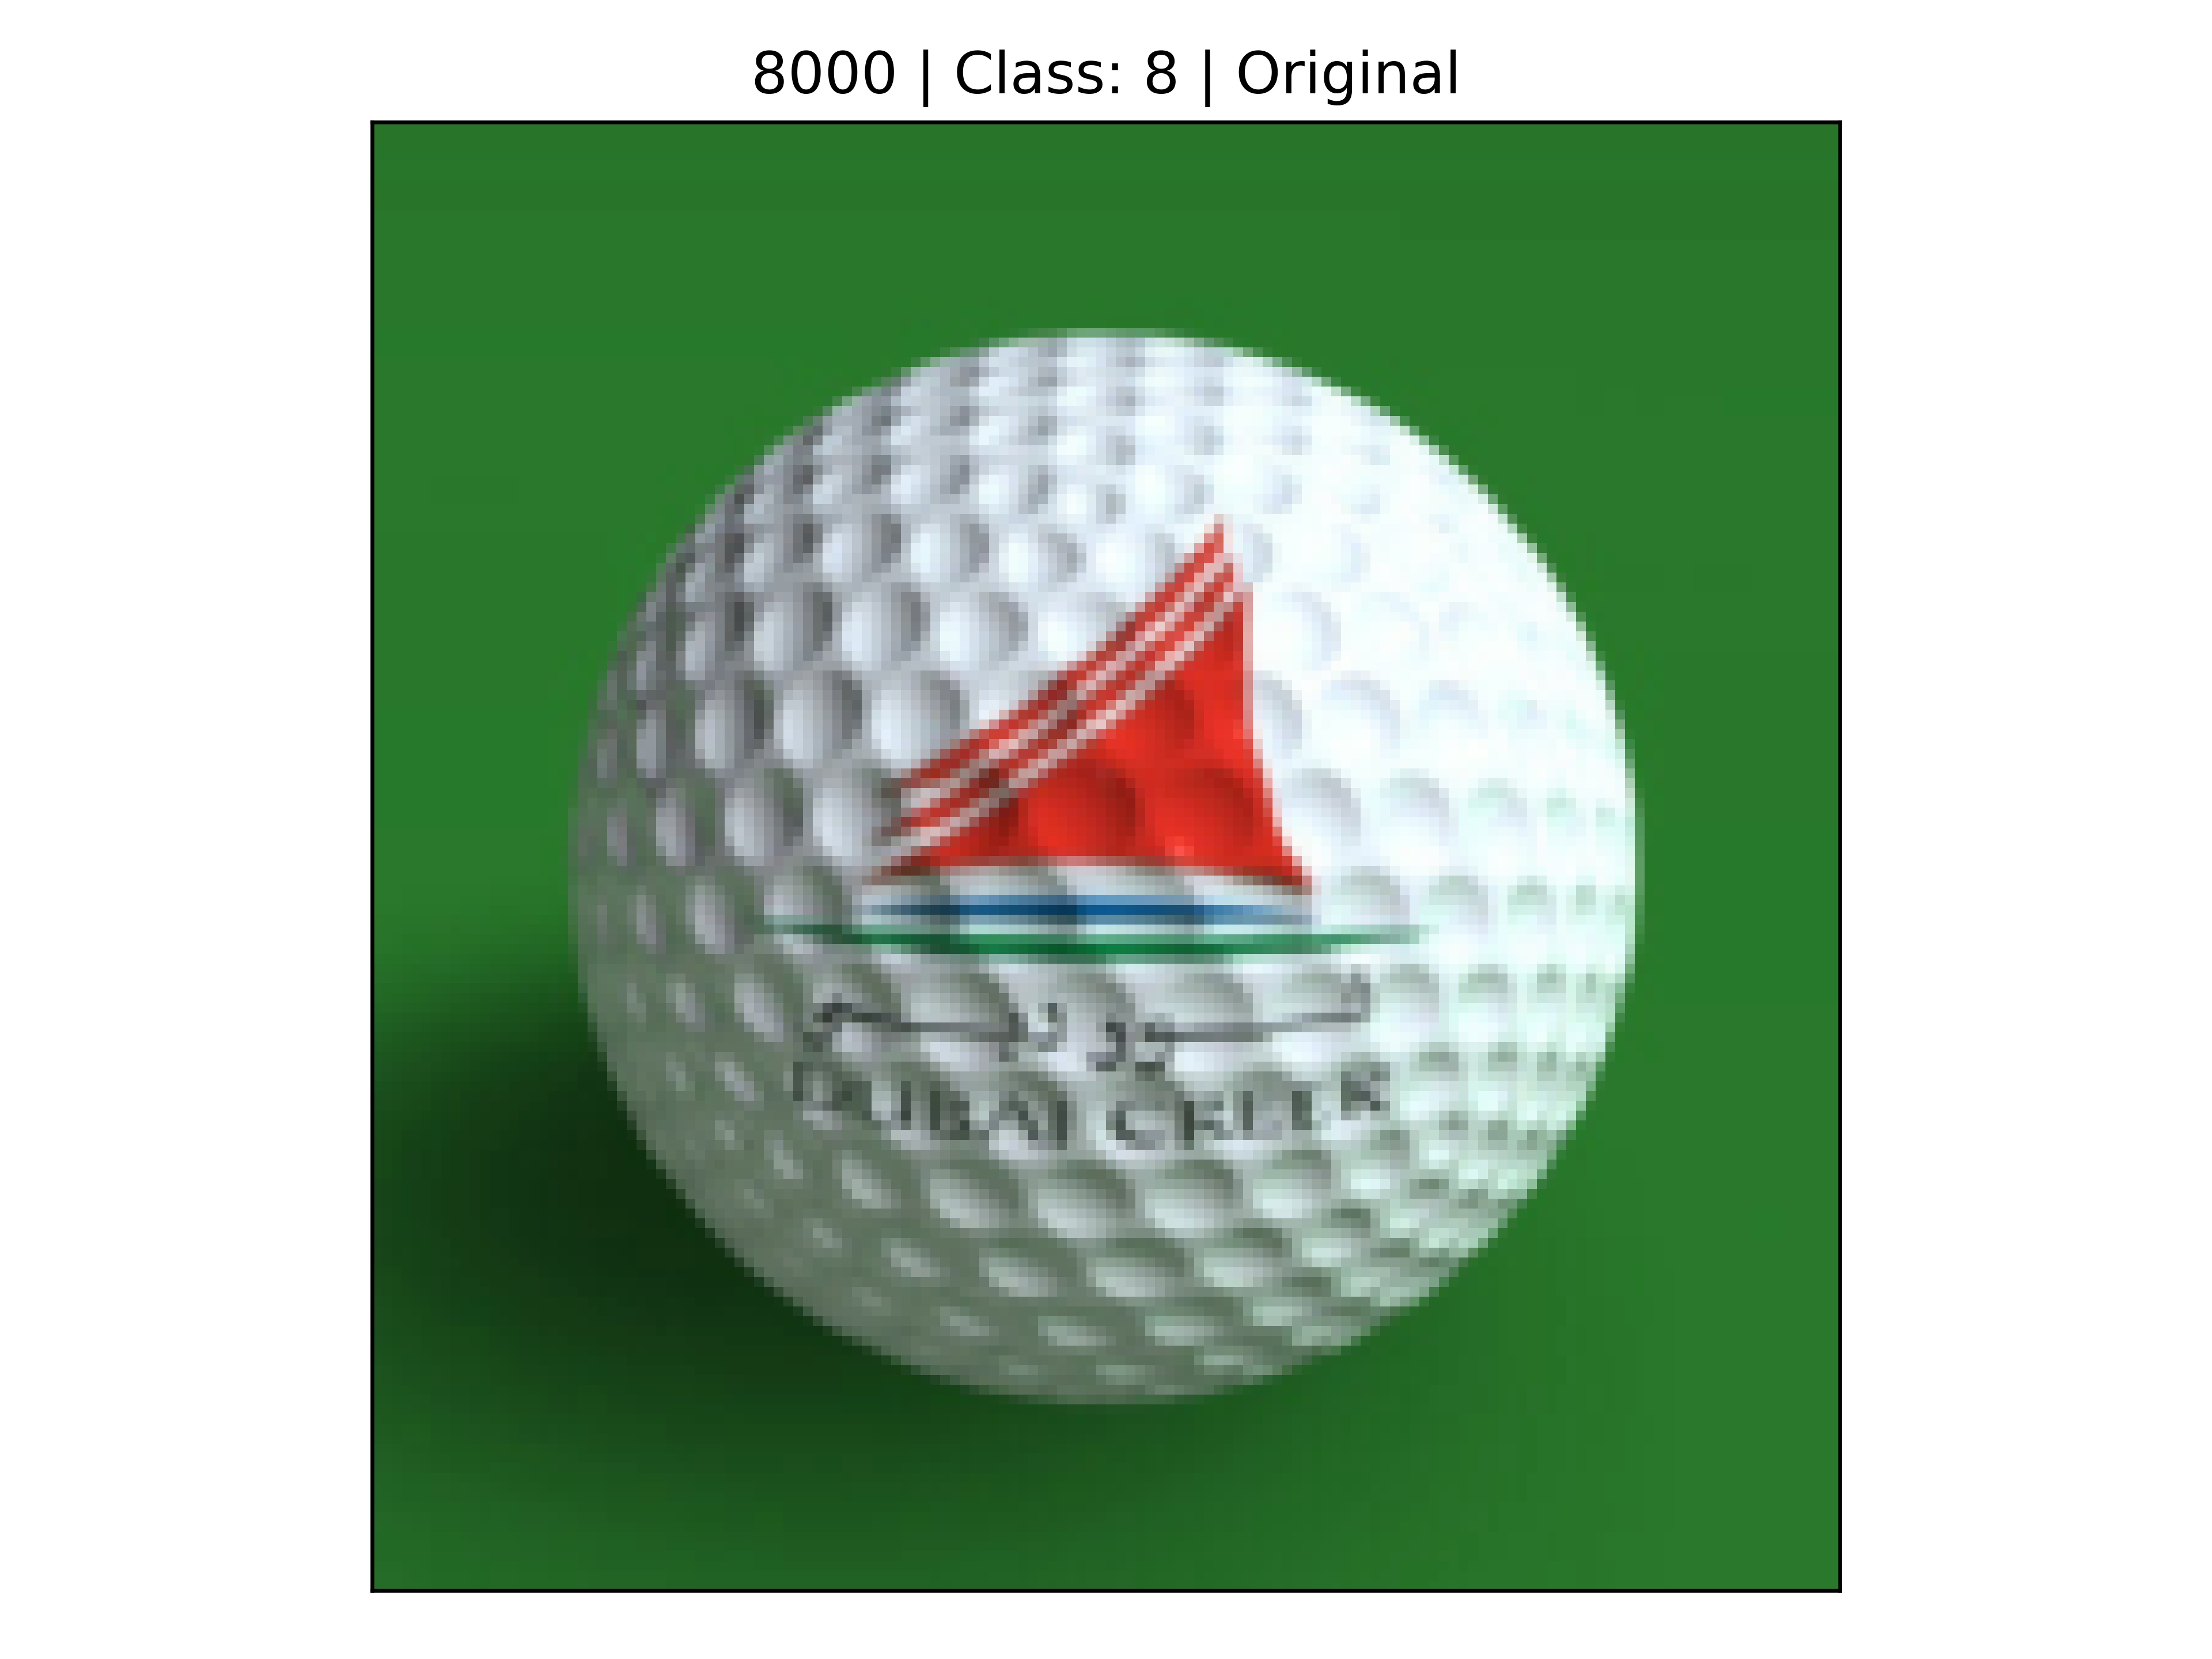
\includegraphics[width=\textwidth]{ch1-diffy/figures/warping_examples/8000.png}
%    \caption{Original}
%    % \label{fig:my_label}
%    \end{subfigure}
%    \caption{Image \#8000. Deformations $\text{warp}(f, T)$ for different values of $T$ ($c=2$).}
%\end{figure}
